\documentclass[11pt, a4paper]{article}
\usepackage[margin=2.5cm]{geometry}
\usepackage{parskip}
\usepackage{titlesec}
\usepackage{hyperref}
\usepackage{enumitem}
\usepackage{booktabs}
\usepackage{array}
\usepackage{graphicx}
\usepackage{amsmath}

\titleformat{\section}{\large\bfseries}{}{0em}{}[\titlerule]
\titleformat{\subsection}{\normalsize\bfseries}{}{0em}{}
\titleformat{\subsubsection}{\normalsize\itshape}{}{0em}{}

\title{\textbf{Monocyte Co-Activation in Severe COVID-19}\\
\large Single-Cell RNA-seq Analysis of PBMC Immune Dysregulation}
\author{}
\date{}

\begin{document}
\maketitle

% ═══════════════════════════════════════════════
\section{Introduction}
% ═══════════════════════════════════════════════

\subsection{Research question}

\begin{quote}
\textit{In severe COVID-19, do blood monocytes enter a pathological state where
they simultaneously activate an antiviral interferon program (ISGs) and a
pro-inflammatory cytokine program (TNF/IL-1$\beta$) — and is this co-activated
state reproducible across independent cohorts?}
\end{quote}

These two programs are:
\begin{itemize}[nosep]
  \item \textbf{Antiviral (ISG) program} — interferon-stimulated genes (ISG15, IFIT1, MX1, OAS1, IFI44L) that fight viral infection.
  \item \textbf{Inflammatory (TNF/IL-1$\beta$) program} — pro-inflammatory cytokines (TNF, IL1B, CCL3, CCL4, CXCL8) that drive aggressive inflammation.
\end{itemize}

A monocyte with \textit{both} programs active simultaneously is called \textbf{co-activated}.
This project tests whether co-activation is real, severity-linked, and reproducible,
using two independent scRNA-seq datasets:
\begin{itemize}[nosep]
  \item \textbf{GSE149689} (Lee et al., \textit{Sci Immunol} 2020) — 20 donors across Healthy, Mild COVID, Severe COVID, and Flu.
  \item \textbf{GSE150861} (Guo et al., \textit{Nat Commun} 2020) — 2 severe COVID patients treated with Tocilizumab, sampled longitudinally.
\end{itemize}

\subsection{Analysis pipeline overview}

The analysis is organized into two parts: a single-cell component (Phases 1--5) and a bulk
RNA-seq component (Phases 7--13), with Phase 6 bridging the two.

\textbf{Single-cell (scRNA-seq):}
\begin{enumerate}[nosep]
  \item \textbf{QC \& Preprocessing} — load raw 10X data, remove low-quality cells.
  \item \textbf{Normalization \& Dimensionality Reduction} — normalize counts, run PCA and UMAP.
  \item \textbf{Clustering \& Cell-Type Annotation} — identify cell populations via graph-based clustering and reference-based annotation.
  \item \textbf{Monocyte Deep-Dive} — subset monocytes, score ISG and TNF/IL-1$\beta$ modules, test co-activation across severity.
  \item \textbf{Independent Replication} — repeat the analysis on GSE150861 to validate findings across a treatment time-series.
\end{enumerate}

\textbf{Bulk RNA-seq (GSE152418):}
\begin{enumerate}[nosep, start=6]
  \item \textbf{Visualization Summary} — consolidate the scRNA-seq story; motivate the bulk question.
  \item \textbf{Bulk EDA} — load 33 whole-blood samples, check quality and confounders.
  \item \textbf{DESeq2 Differential Expression} — identify genes changing in Severe/ICU blood.
  \item \textbf{Confounder Correction} — adjust for gender imbalance; validate robustness.
  \item \textbf{Bulk Visualization} — directly test whether co-activation genes are detectable in blood.
  \item \textbf{PCA \& Clustering} — confirm the DE signal at the whole-transcriptome level (unsupervised).
  \item \textbf{GSEA} — identify biological programs, not just individual genes, driving the difference.
  \item \textbf{ssGSEA Signature Test} — final sensitivity test for the co-activation signal in bulk.
\end{enumerate}

% ═══════════════════════════════════════════════
\section{Phase 1 — Quality Control and Preprocessing}
% ═══════════════════════════════════════════════

\subsection{Data loading}

The raw count matrix from GSE149689 was loaded via \texttt{Read10X()}.
The matrix contains \textbf{33,538 genes $\times$ 85,144 cells} with 95.6\% sparsity
(typical for scRNA-seq — most genes are not expressed in any given cell).
After removing genes expressed in fewer than 3 cells, a Seurat object was created
with \textbf{23,335 genes $\times$ 85,144 cells}.

\subsection{QC metrics and filtering}

Three quality metrics were computed per cell:
\textbf{nFeature\_RNA} (genes detected), \textbf{nCount\_RNA} (total UMIs),
and \textbf{percent.mt} (mitochondrial RNA fraction, indicating cell damage).

\begin{center}
  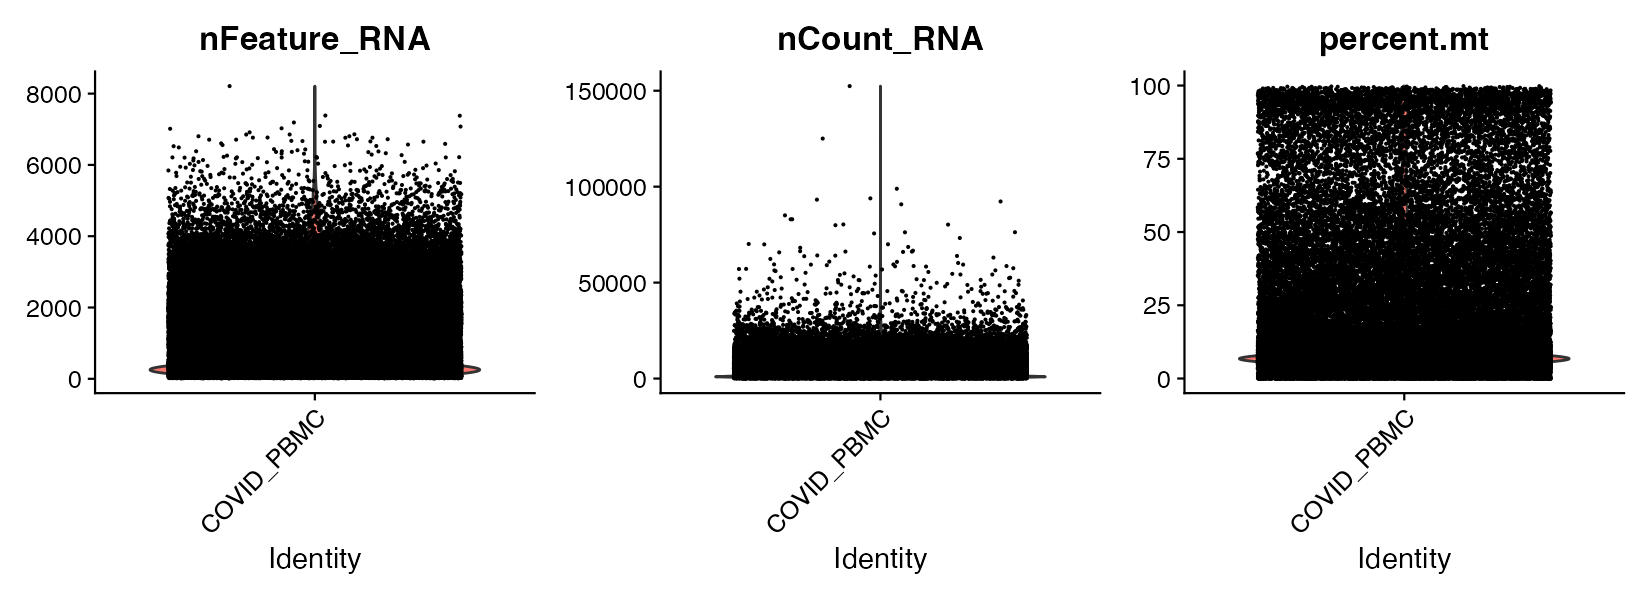
\includegraphics[width=\textwidth]{plots/phase1/phase1_step08_violin_qc_metrics.png}
\end{center}

The violin plots reveal:
\begin{itemize}[nosep]
  \item A dense mass of low-gene-count cells (empty droplets) compressed near zero in nFeature\_RNA.
  \item A heavy tail extending to 100\% in percent.mt — $\sim$25\% of cells have $>$20\% mitochondrial content, consistent with cell stress in severely ill COVID-19 patients.
  \item A small number of high-count outliers (doublet candidates) above 6,000 genes.
\end{itemize}

Cells were filtered using five thresholds:
nFeature\_RNA $\in [500, 6000]$, nCount\_RNA $\in [1000, 40000]$, percent.mt $< 20\%$.

\begin{center}
  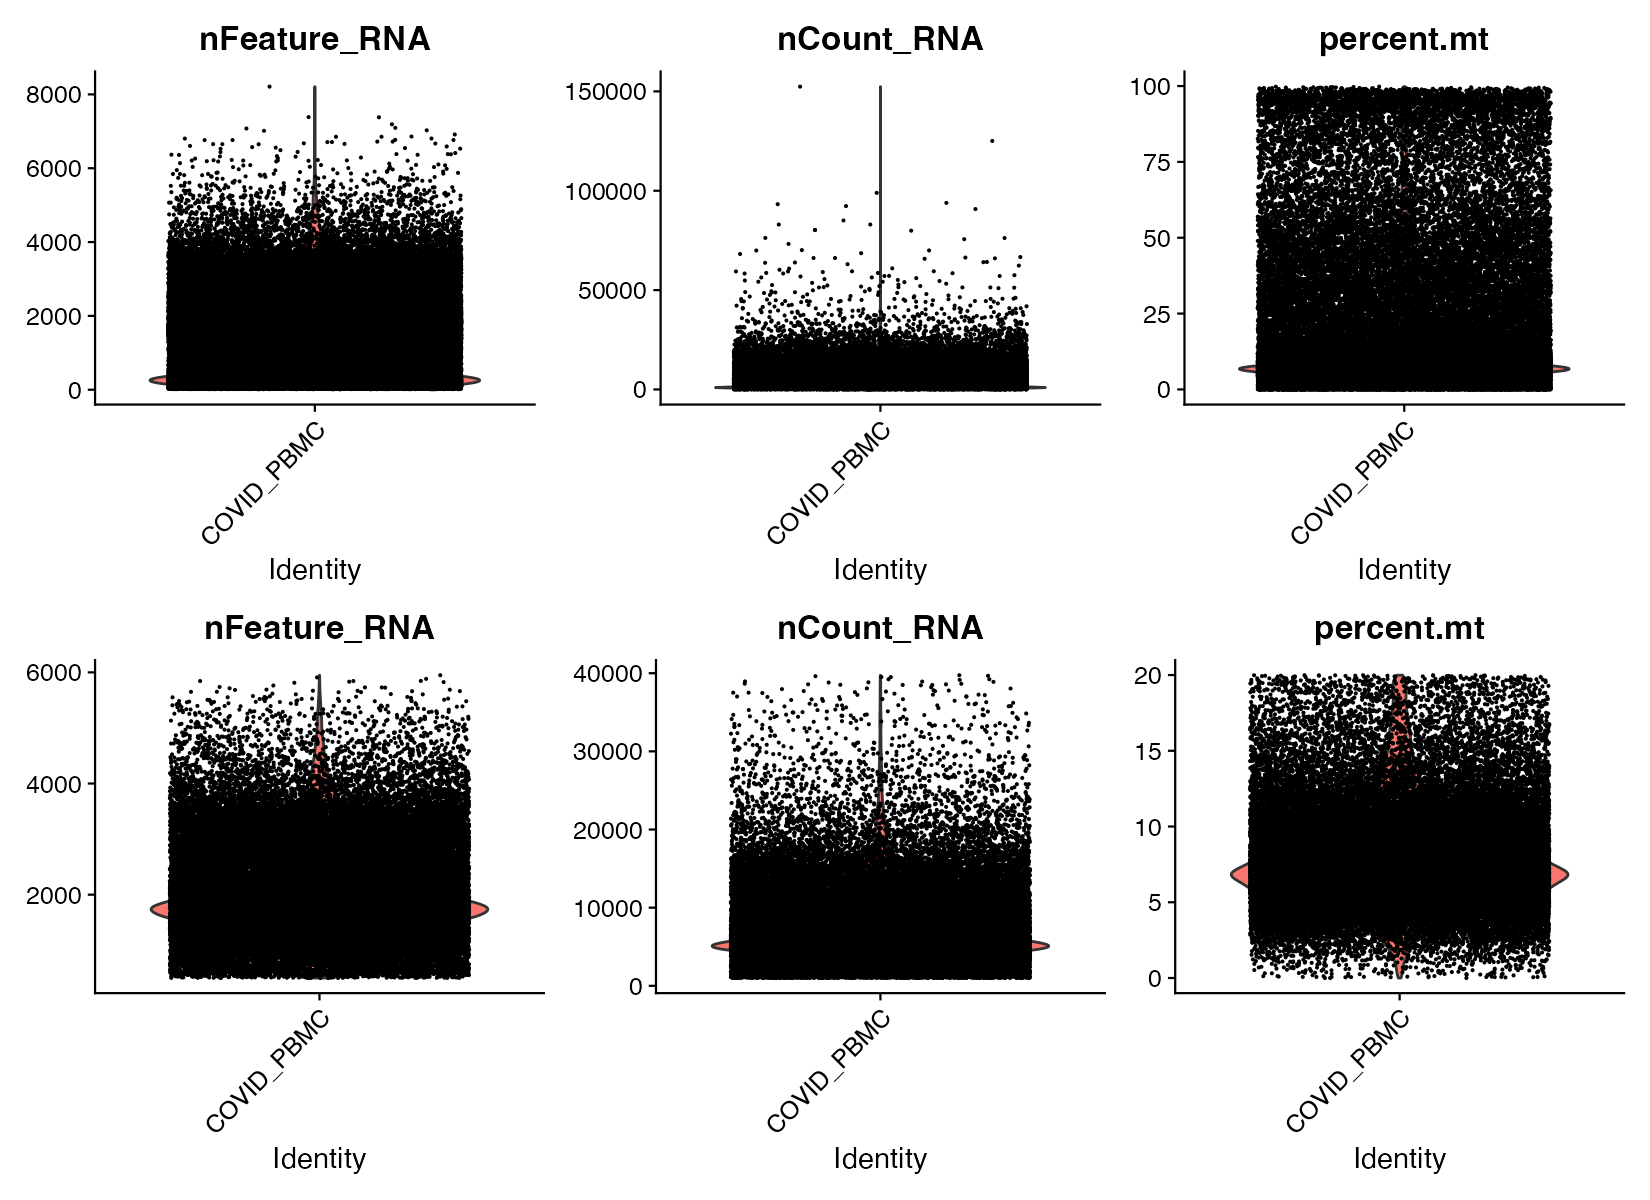
\includegraphics[width=\textwidth]{plots/phase1/phase1_step11_before_after_filtering.png}
\end{center}

Filtering removed \textbf{29,596 cells (34.8\%)}, retaining \textbf{55,548 cells}.
The before/after comparison shows the removal of the low-gene mass and the high-mito tail.
After filtering, the typical cell has 1,872 detected genes, 5,845 UMIs, and 7.3\% mitochondrial RNA — all healthy values.

The high proportion of damaged cells in the raw data is itself informative:
it reflects the stressed immune environment in blood from severely ill patients.

% ═══════════════════════════════════════════════
\section{Phase 2 — Normalization and Dimensionality Reduction}
% ═══════════════════════════════════════════════

\subsection{Normalization and feature selection}

Raw counts were log-normalized (\texttt{NormalizeData}, scale factor 10,000),
the 3,000 most variable genes were selected (\texttt{FindVariableFeatures}, VST method),
and data were scaled with regression of percent.mt to remove the confounding
effect of cell stress on downstream analysis.

\textit{Note: SCTransform was attempted but exceeded memory limits on this dataset (55K cells).
LogNormalize is well-validated and widely used.}

\subsection{PCA and choosing the number of components}

PCA was run on the 3,000 variable genes. The elbow plot below shows the
standard deviation of each PC — the curve flattens around PC\,20, marking
the transition from biological signal to noise.

\begin{center}
  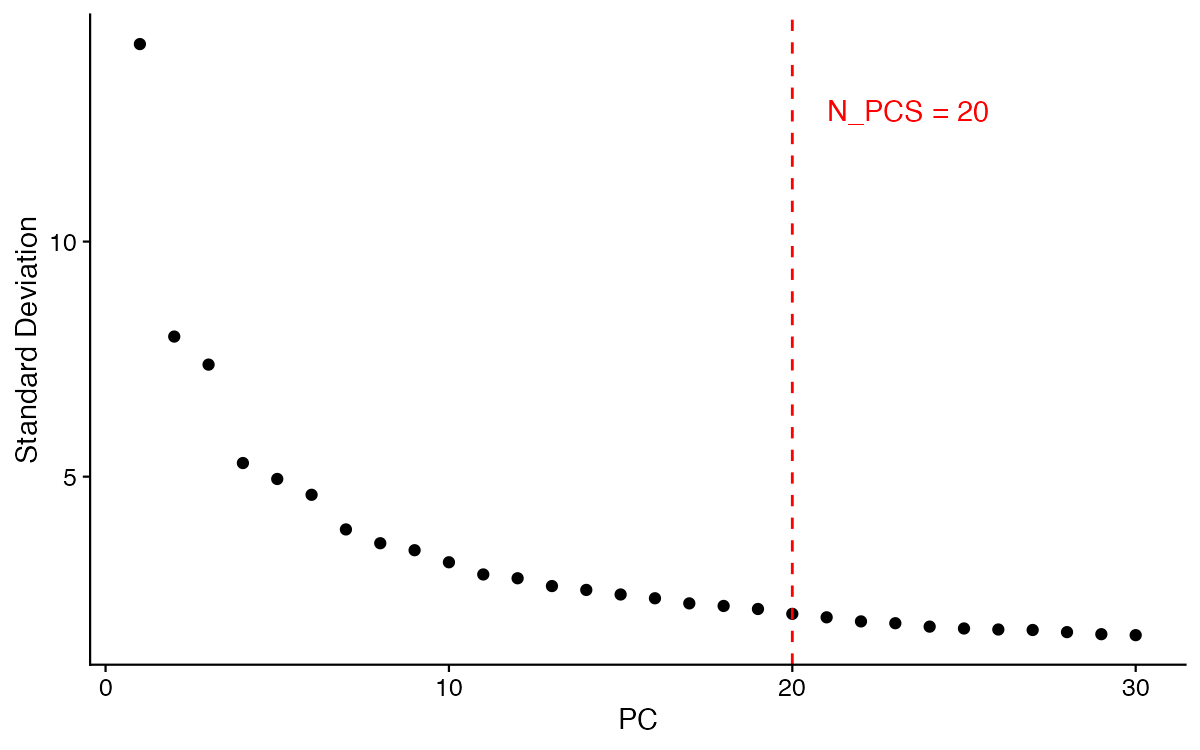
\includegraphics[width=0.85\textwidth]{plots/phase2/phase2_step06_elbow_plot.png}
\end{center}

PC loadings confirm biologically meaningful axes: PC1 separates monocytes (FCN1, LYZ, S100A9),
PC2 captures a platelet signal (CLEC1B, TUBB1), and PC3 separates B cells from NK/T cells
(CD79A vs NKG7). \textbf{Decision: 20 PCs} retained for downstream embedding and clustering.

\subsection{UMAP embedding}

UMAP was computed from the first 20 PCs to project 55,548 cells into 2D.

\begin{center}
  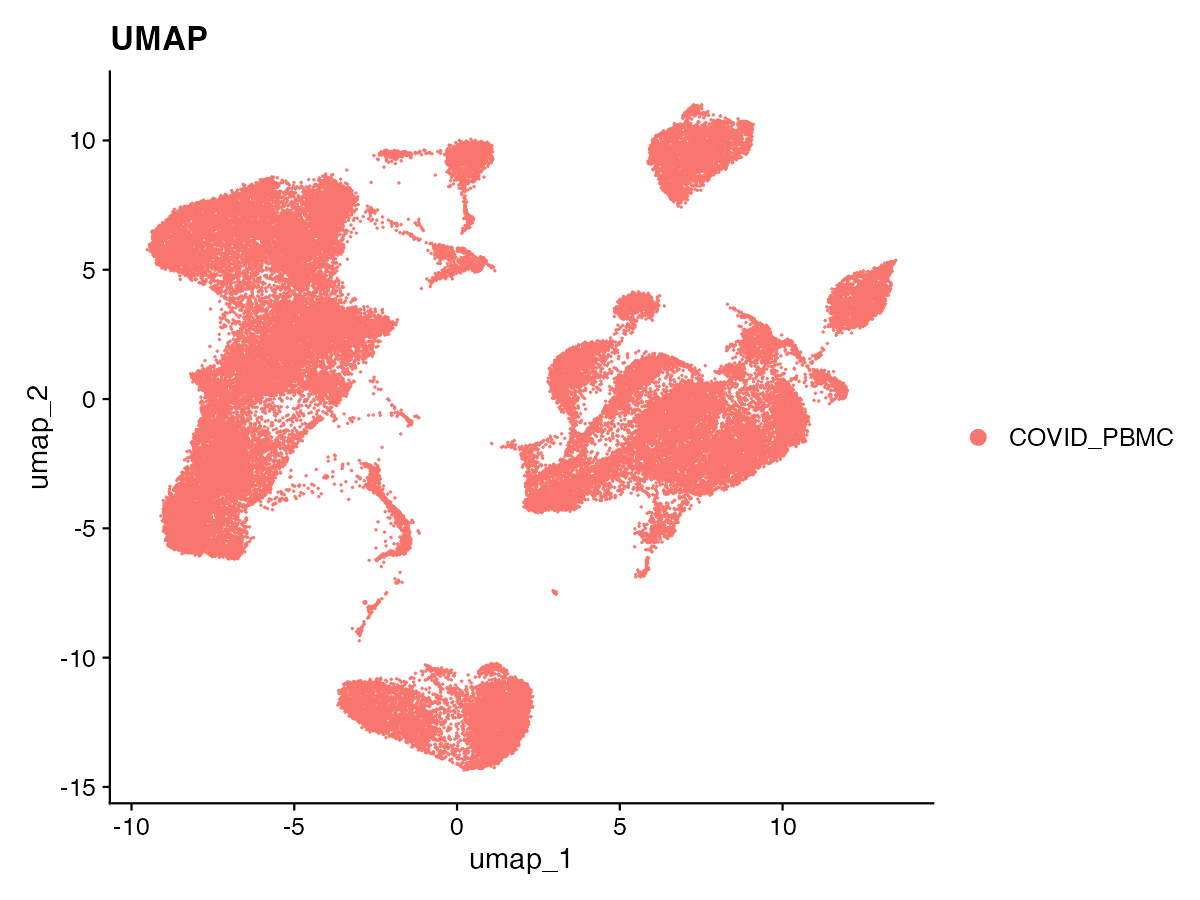
\includegraphics[width=0.85\textwidth]{plots/phase2/phase2_step07_umap.png}
\end{center}

The UMAP shows well-separated clusters with clear gaps between groups.
Before any annotation, the topology already suggests distinct cell populations —
a large myeloid continent, separated lymphoid islands, and isolated rare populations.
Phase 3 will assign identities.

% ═══════════════════════════════════════════════
\section{Phase 3 — Clustering and Cell-Type Annotation}
% ═══════════════════════════════════════════════

\subsection{Graph-based clustering}

A shared-nearest-neighbor (SNN) graph was built from the 20-PC embedding
(\texttt{FindNeighbors}), and clusters were detected with the Louvain algorithm
(\texttt{FindClusters}) at multiple resolutions.

Resolution 0.5 yielded \textbf{23 clusters} — the best balance between capturing
distinct sub-populations and avoiding over-fragmentation.
Higher resolutions (0.8, 1.0) showed instability (cluster count dropped from 35 to 34),
a sign of over-splitting.

\begin{center}
  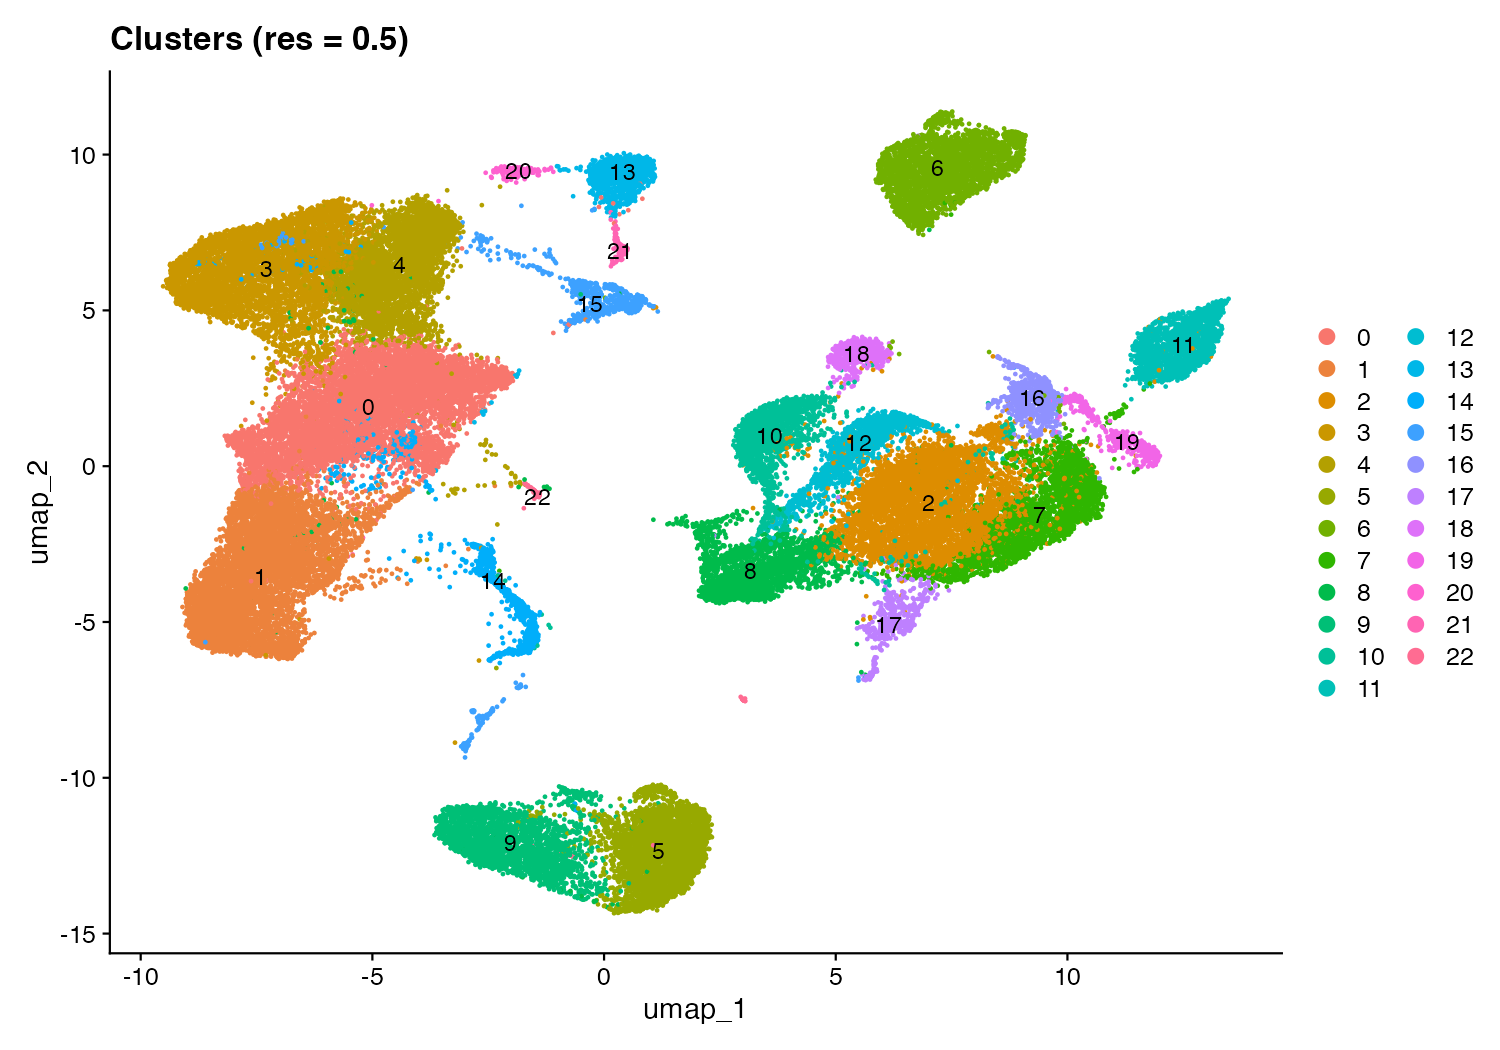
\includegraphics[width=0.9\textwidth]{plots/phase3/phase3_step07a_umap_clusters_final.png}
\end{center}

\subsection{Marker gene validation}

A dot plot of 14 canonical markers across all 23 clusters reveals clear cell-type identities.
Dot size = fraction of cells expressing the gene; colour = mean scaled expression.

\begin{center}
  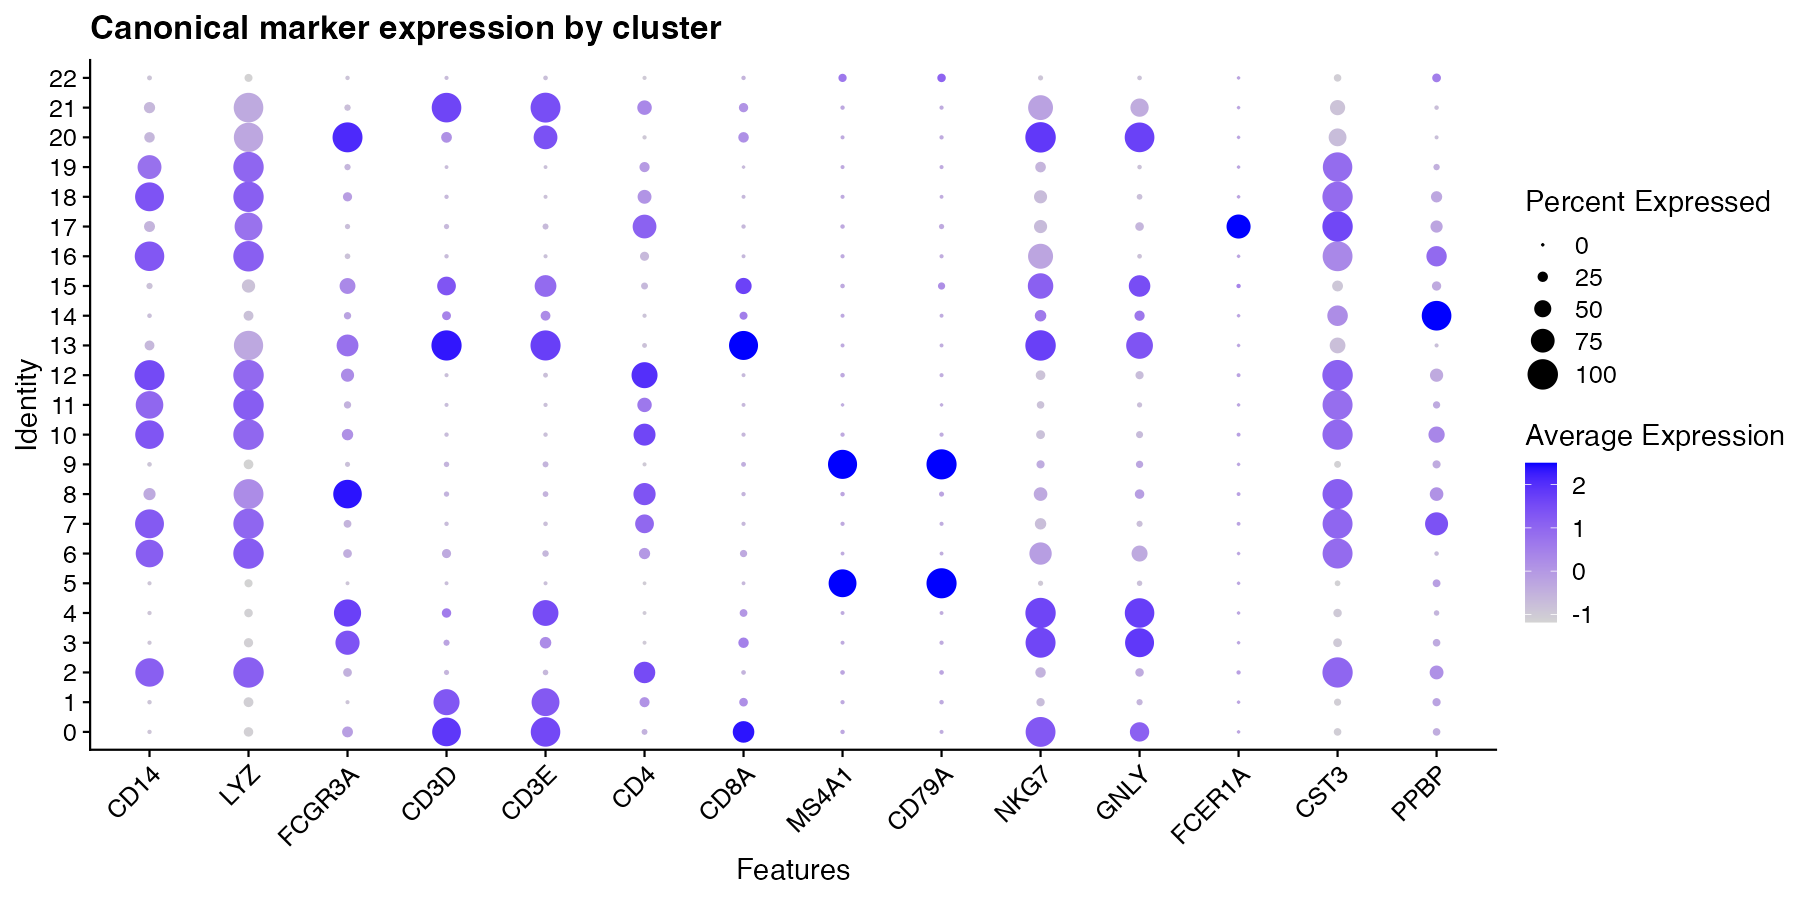
\includegraphics[width=\textwidth]{plots/phase3/phase3_step08e_dotplot_markers.png}
\end{center}

Reading across clusters:
\begin{itemize}[nosep]
  \item \textbf{Clusters 2, 6, 7, 8, 10--12, 16, 18, 19}: high CD14/LYZ → \textbf{monocyte sub-clusters} (classical, non-classical, inflammatory, ISG-high, etc.)
  \item \textbf{Clusters 0, 13}: high CD8A, NKG7 → \textbf{CD8$^+$ T / NK cells}
  \item \textbf{Cluster 1}: high CD3D, CD4 → \textbf{CD4$^+$ T cells}
  \item \textbf{Clusters 3, 4, 20}: high NKG7, GNLY → \textbf{NK cells}
  \item \textbf{Clusters 5, 9}: high MS4A1, CD79A → \textbf{B cells}
  \item \textbf{Cluster 14}: high PPBP → \textbf{platelets}
  \item \textbf{Cluster 17}: FCER1A → \textbf{dendritic cells}
\end{itemize}

\subsection{Automated annotation with SingleR}

SingleR compared each cell's full expression profile against the BlueprintEncode
reference to assign cell-type labels independently of the clustering.

\begin{center}
  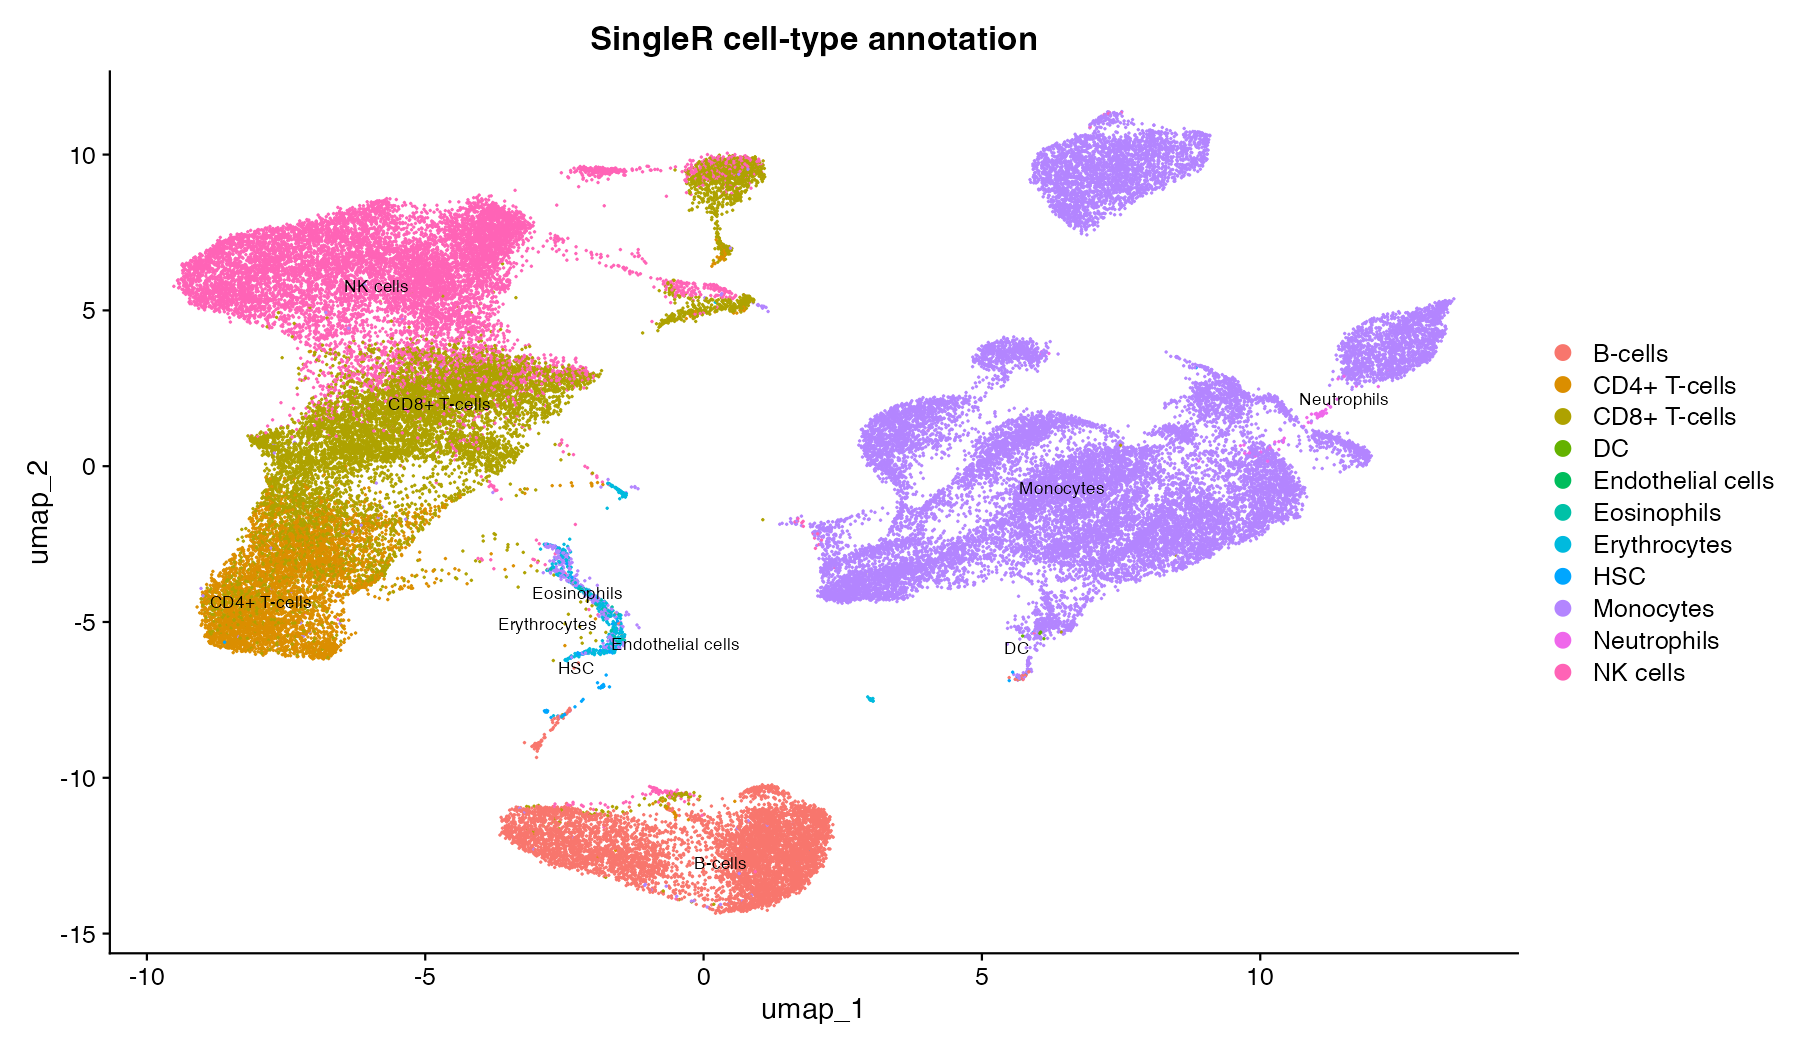
\includegraphics[width=0.95\textwidth]{plots/phase3/phase3_step09c_umap_singler.png}
\end{center}

SingleR labels agree with the marker-based identities on all major populations.
The five PBMC compartments are cleanly resolved:
monocytes (38.5\%), NK cells (20.5\%), CD8$^+$ T cells (18.8\%), B cells (12.0\%),
and CD4$^+$ T cells (9.0\%).

The monocyte dominance (38.5\%) and CD4$^+$ T cell depletion (9.0\%) are
established hallmarks of COVID-19 in PBMC datasets.

Notably, 10 of the 23 clusters are monocyte sub-clusters — including
IL-1$\beta^+$ inflammasome-active monocytes (cluster 7),
ISG-high interferon-stimulated monocytes (cluster 10),
and CCL2$^+$/CXCL10$^+$ chemokine-secreting monocytes (cluster 18).
This diversity of monocyte states motivates the deep-dive in Phase 4.

% ═══════════════════════════════════════════════
\section{Phase 4 — CD14$^+$ Monocyte Deep-Dive}
% ═══════════════════════════════════════════════

This is the core analysis: testing whether monocytes in severe COVID-19
run both the antiviral and inflammatory programs simultaneously.

\subsection{Severity metadata and composition shifts}

Each of the 55,548 cells was assigned a severity label based on donor identity
(from Lee et al.\ Table S1): \textbf{Healthy} (4 donors), \textbf{Mild COVID} (4 donors),
\textbf{Severe COVID} (7 donors), and \textbf{Flu} (5 donors).

\begin{center}
  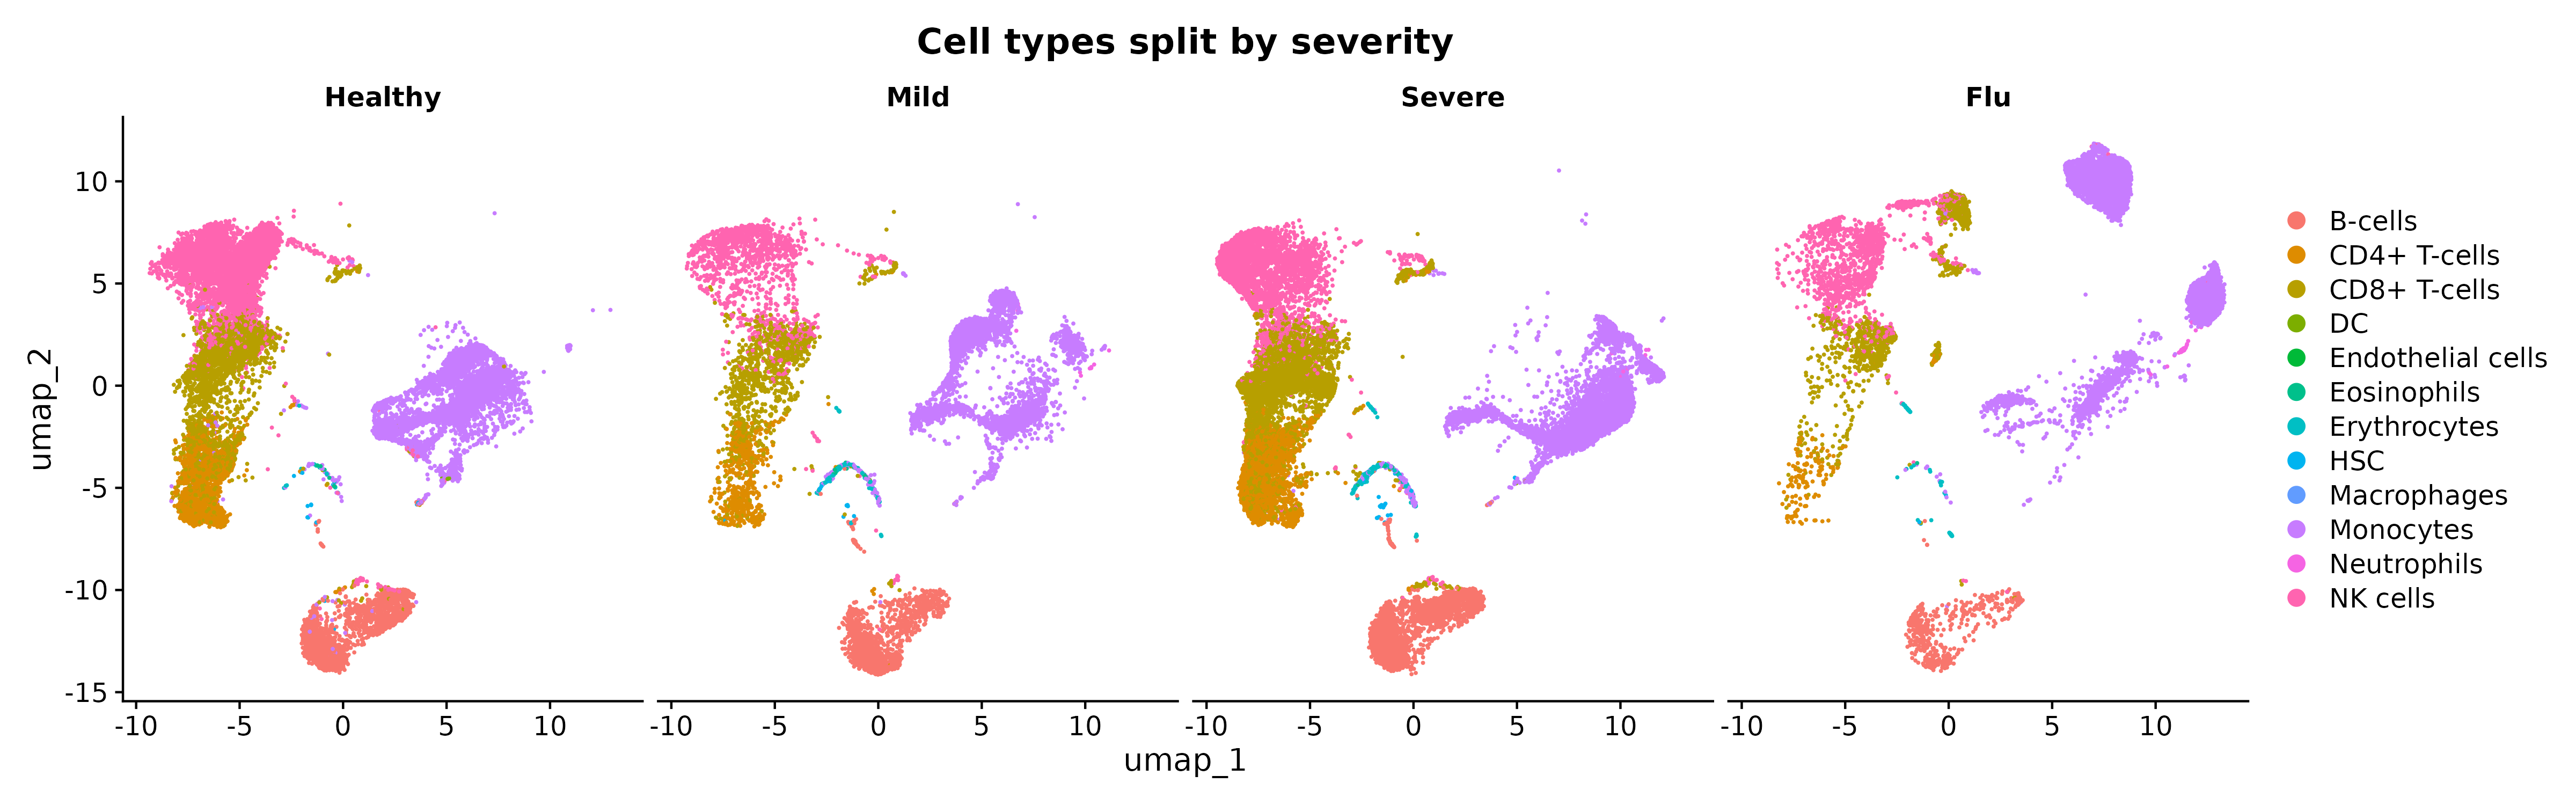
\includegraphics[width=\textwidth]{plots/phase4/phase4_umap_split_severity.png}
\end{center}

Splitting the UMAP by severity reveals a clear compositional shift:
the monocyte mass (right) grows denser from Healthy to Severe,
while the lymphoid continent (left) thins — visual evidence of the
monocyte expansion and T cell depletion characteristic of severe COVID-19.

\begin{center}
  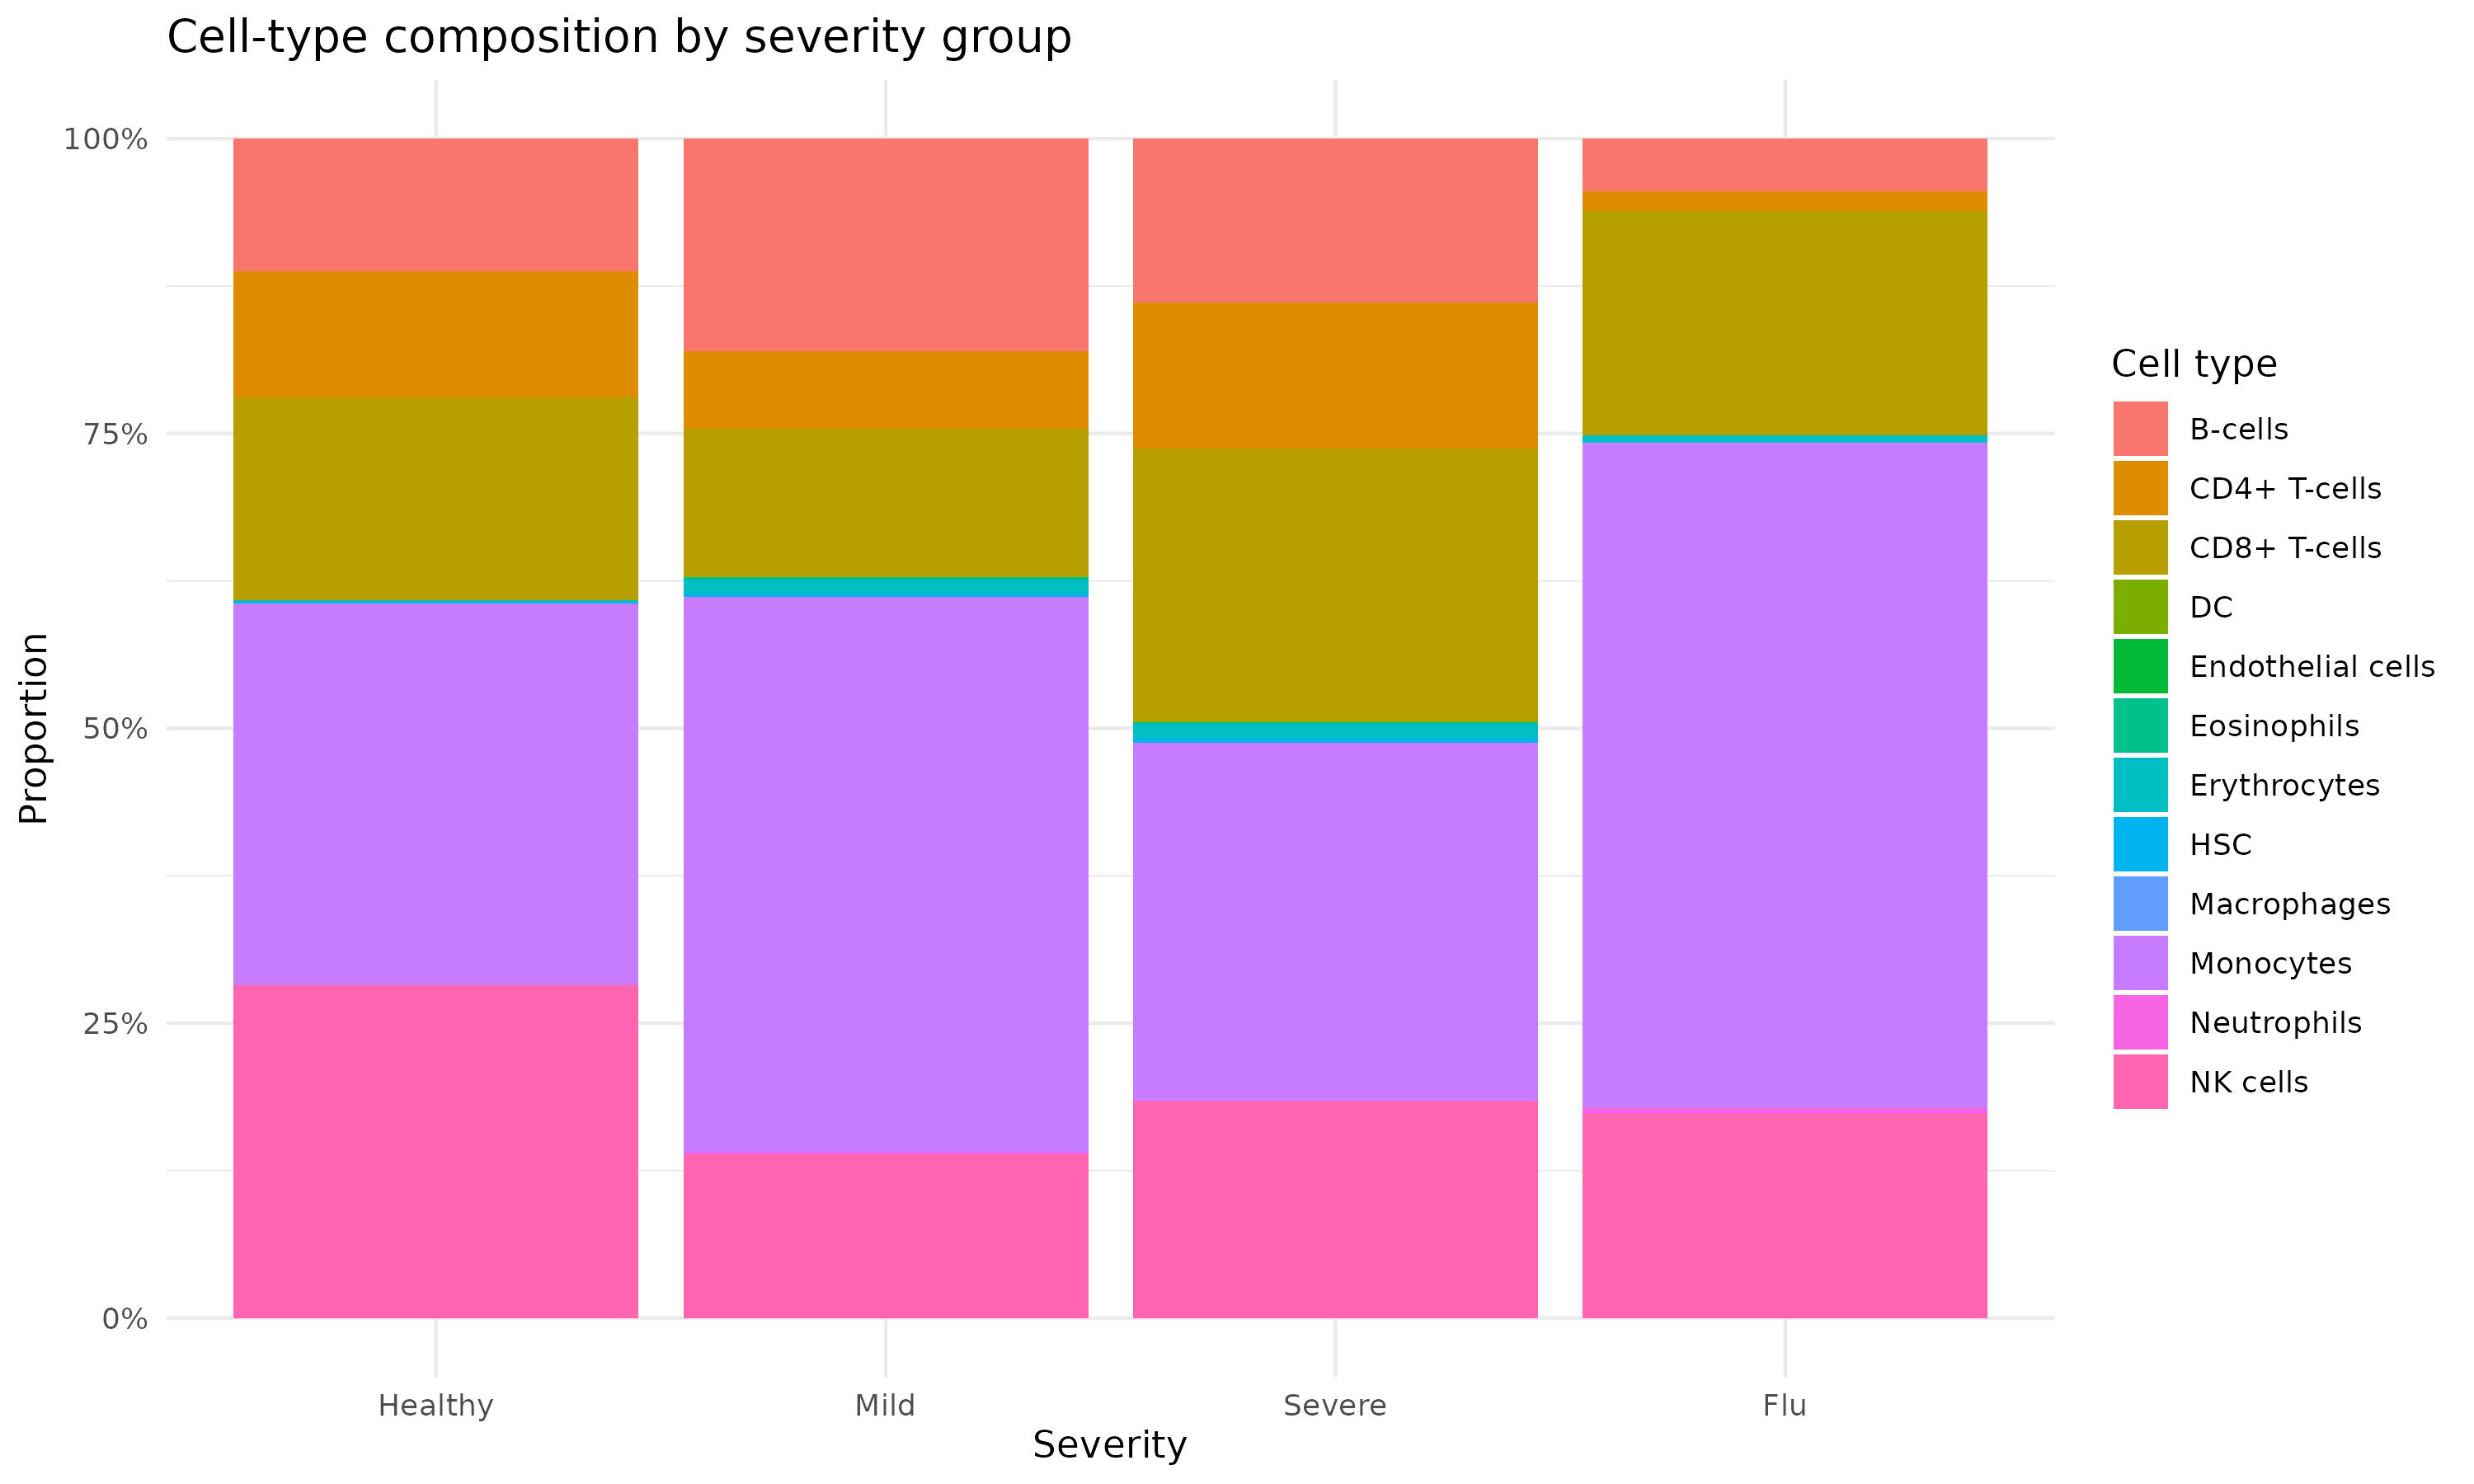
\includegraphics[width=0.9\textwidth]{plots/phase4/phase4_composition_barplot.png}
\end{center}

The stacked barplot quantifies this: monocytes increase from $\sim$35\% (Healthy)
to $\sim$50\% (Severe) while CD4$^+$ T cells drop from $\sim$12\% to $\sim$5\%.
Severe COVID reshapes the blood immune landscape, motivating a focused
analysis of the expanding monocyte compartment.

\subsection{Module scoring and co-activation}

All 21,385 monocytes were subset and scored for two gene modules using
Seurat's \texttt{AddModuleScore}:
\begin{itemize}[nosep]
  \item \textbf{ISG score}: ISG15, IFIT1, MX1, OAS1, IFI44L
  \item \textbf{TNF/IL-1$\beta$ score}: TNF, IL1B, CCL3, CCL4, CXCL8
\end{itemize}

A cell is \textbf{co-activated} when both scores exceed zero simultaneously.

\begin{center}
  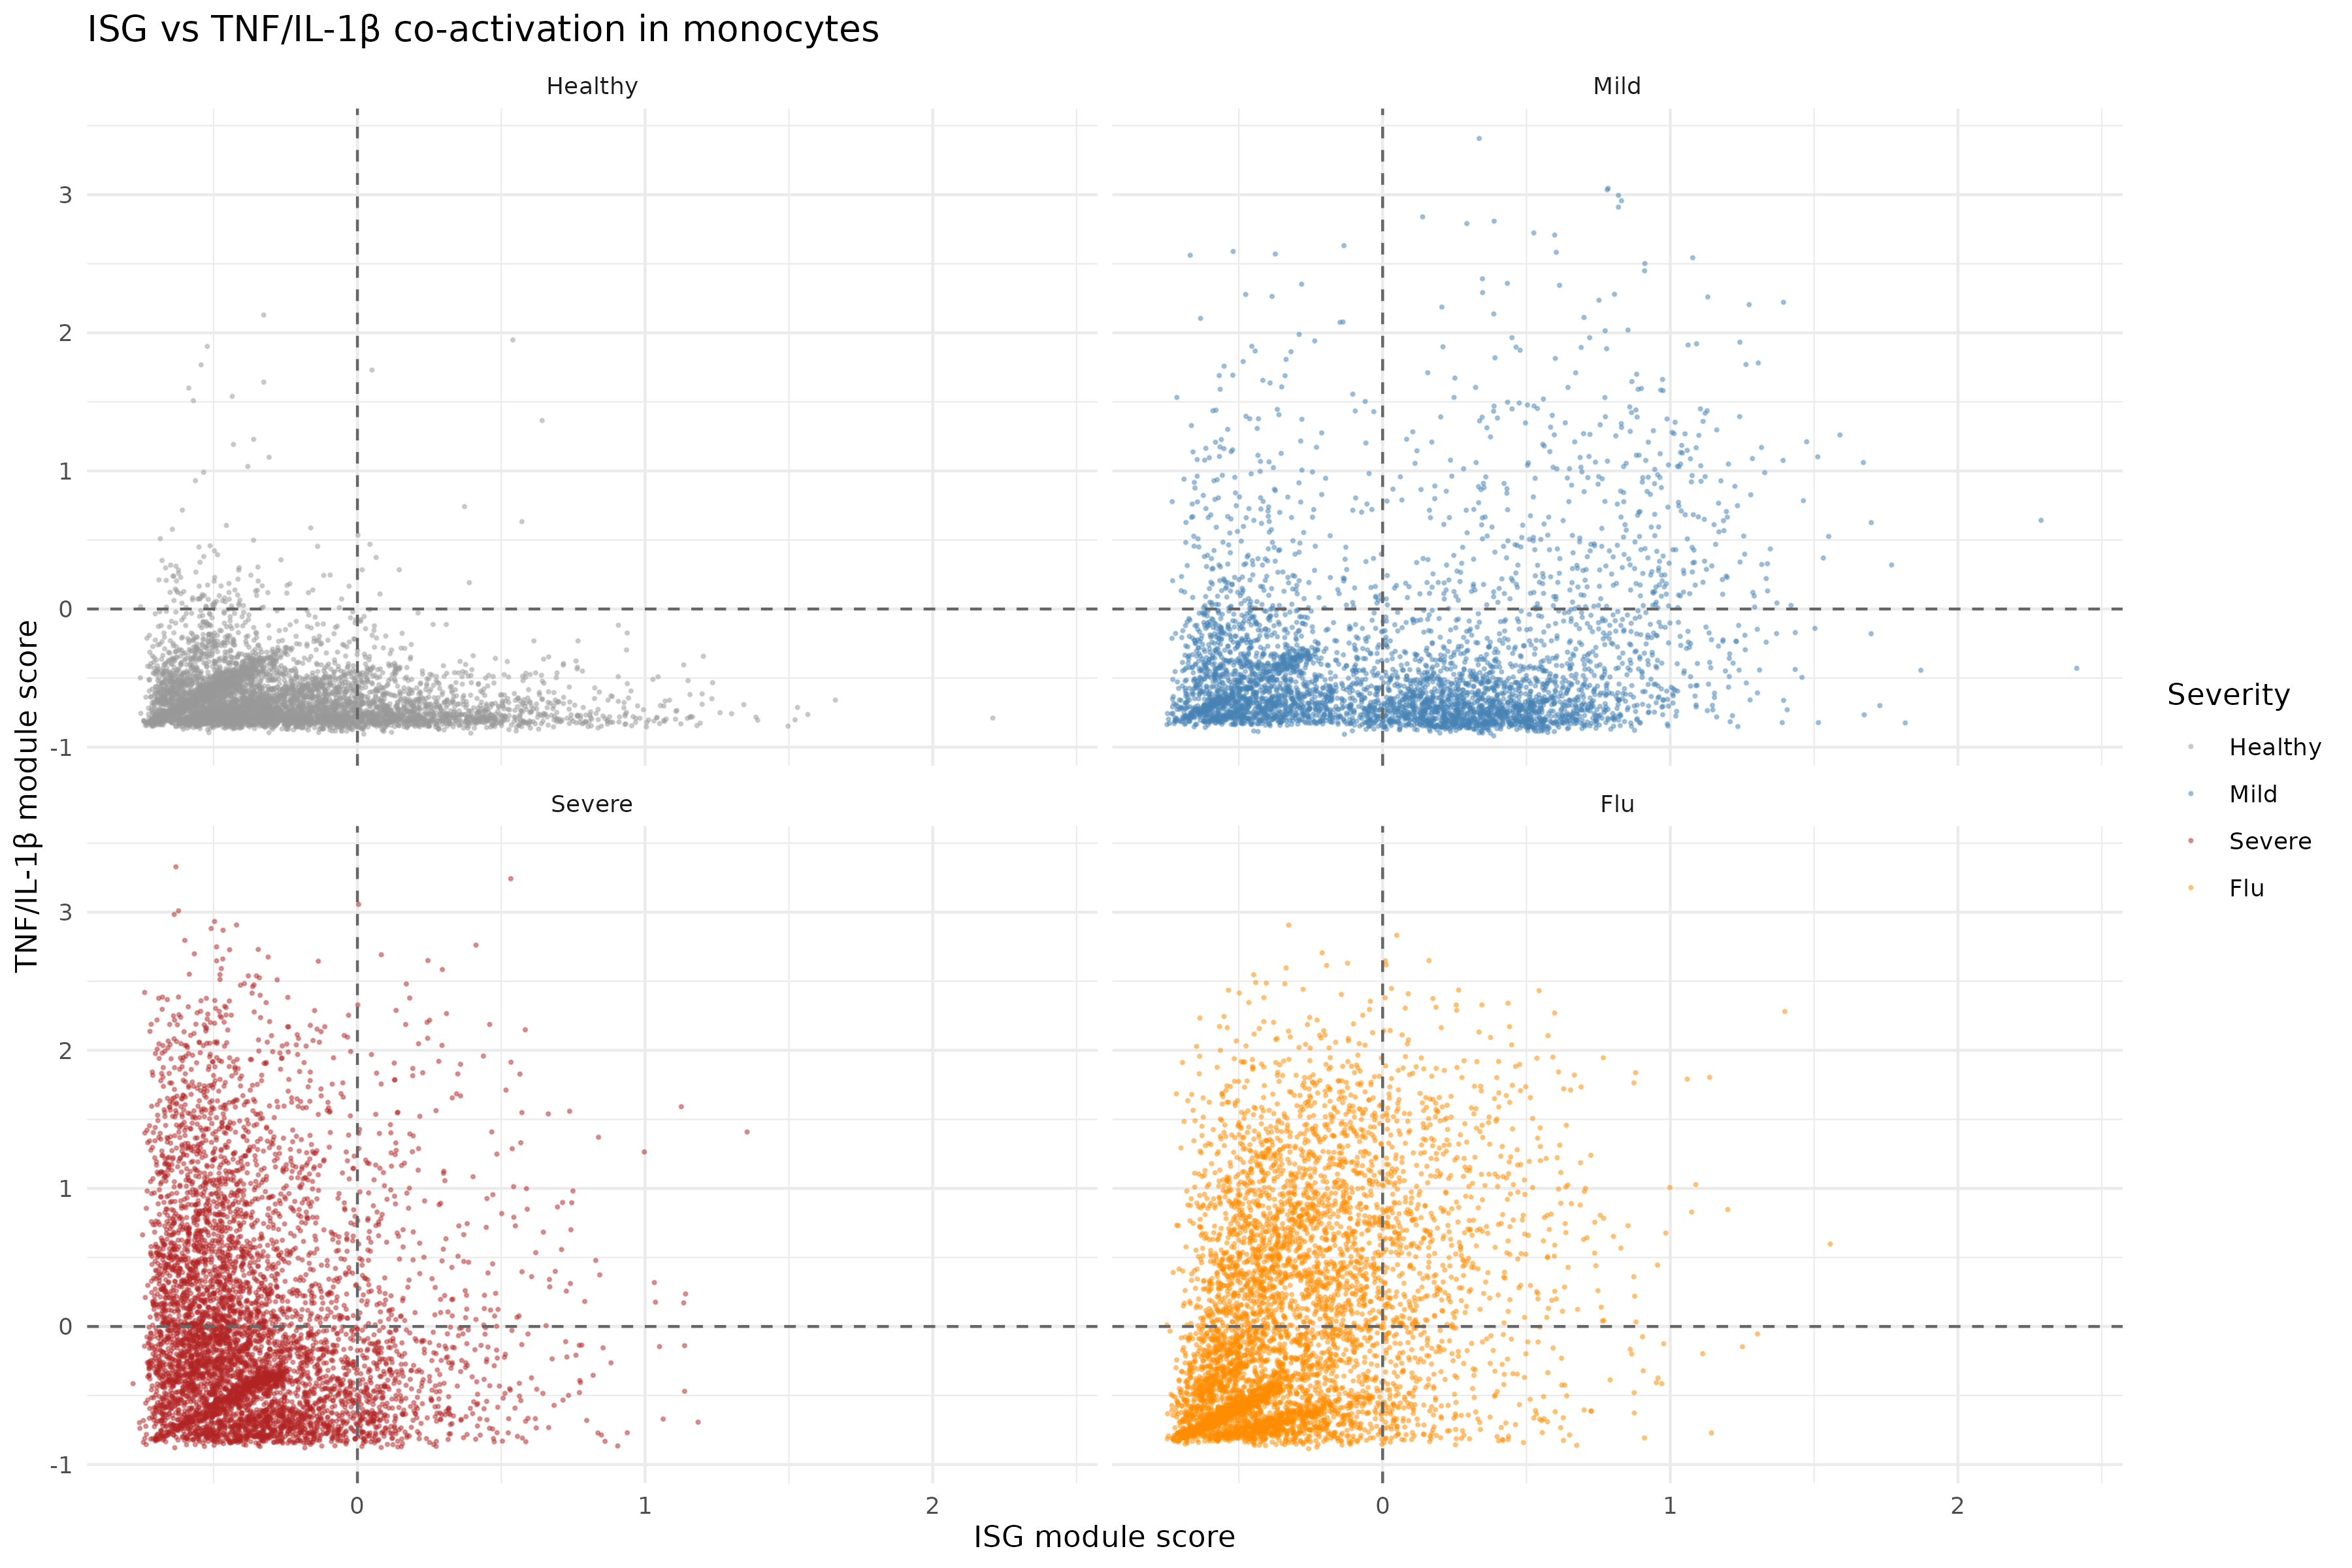
\includegraphics[width=\textwidth]{plots/phase4/phase4_coactivation_scatter.png}
\end{center}

\textbf{This is the central figure of the project.}
Each dot is one monocyte; dashed lines at $x=0$ and $y=0$ divide the plot
into four quadrants (resting, ISG-only, inflammatory-only, co-activated).

Key observations:
\begin{itemize}[nosep]
  \item \textbf{Healthy}: cells cluster tightly in the bottom-left (both programs off).
  \item \textbf{Mild}: cells spread into all quadrants, including the co-activated top-right. Mild COVID shows the strongest ISG activation at the cell level.
  \item \textbf{Severe}: the cell cloud shifts \textit{upward and left} — high TNF/IL-1$\beta$ but lower ISG. Many cells run pure inflammation without antiviral defense.
  \item \textbf{Flu}: similar pattern to Severe, with a large upper-left mass.
\end{itemize}

The co-activated state exists in all infected conditions but is virtually absent in Healthy.
Crucially, while Mild COVID monocytes tend toward ISG-high states,
Severe COVID monocytes shift toward unchecked inflammation.

\subsection{Donor-level statistical comparison}

Since cells from the same donor are not independent, we aggregate to donor-level
means for statistical testing.

\begin{center}
  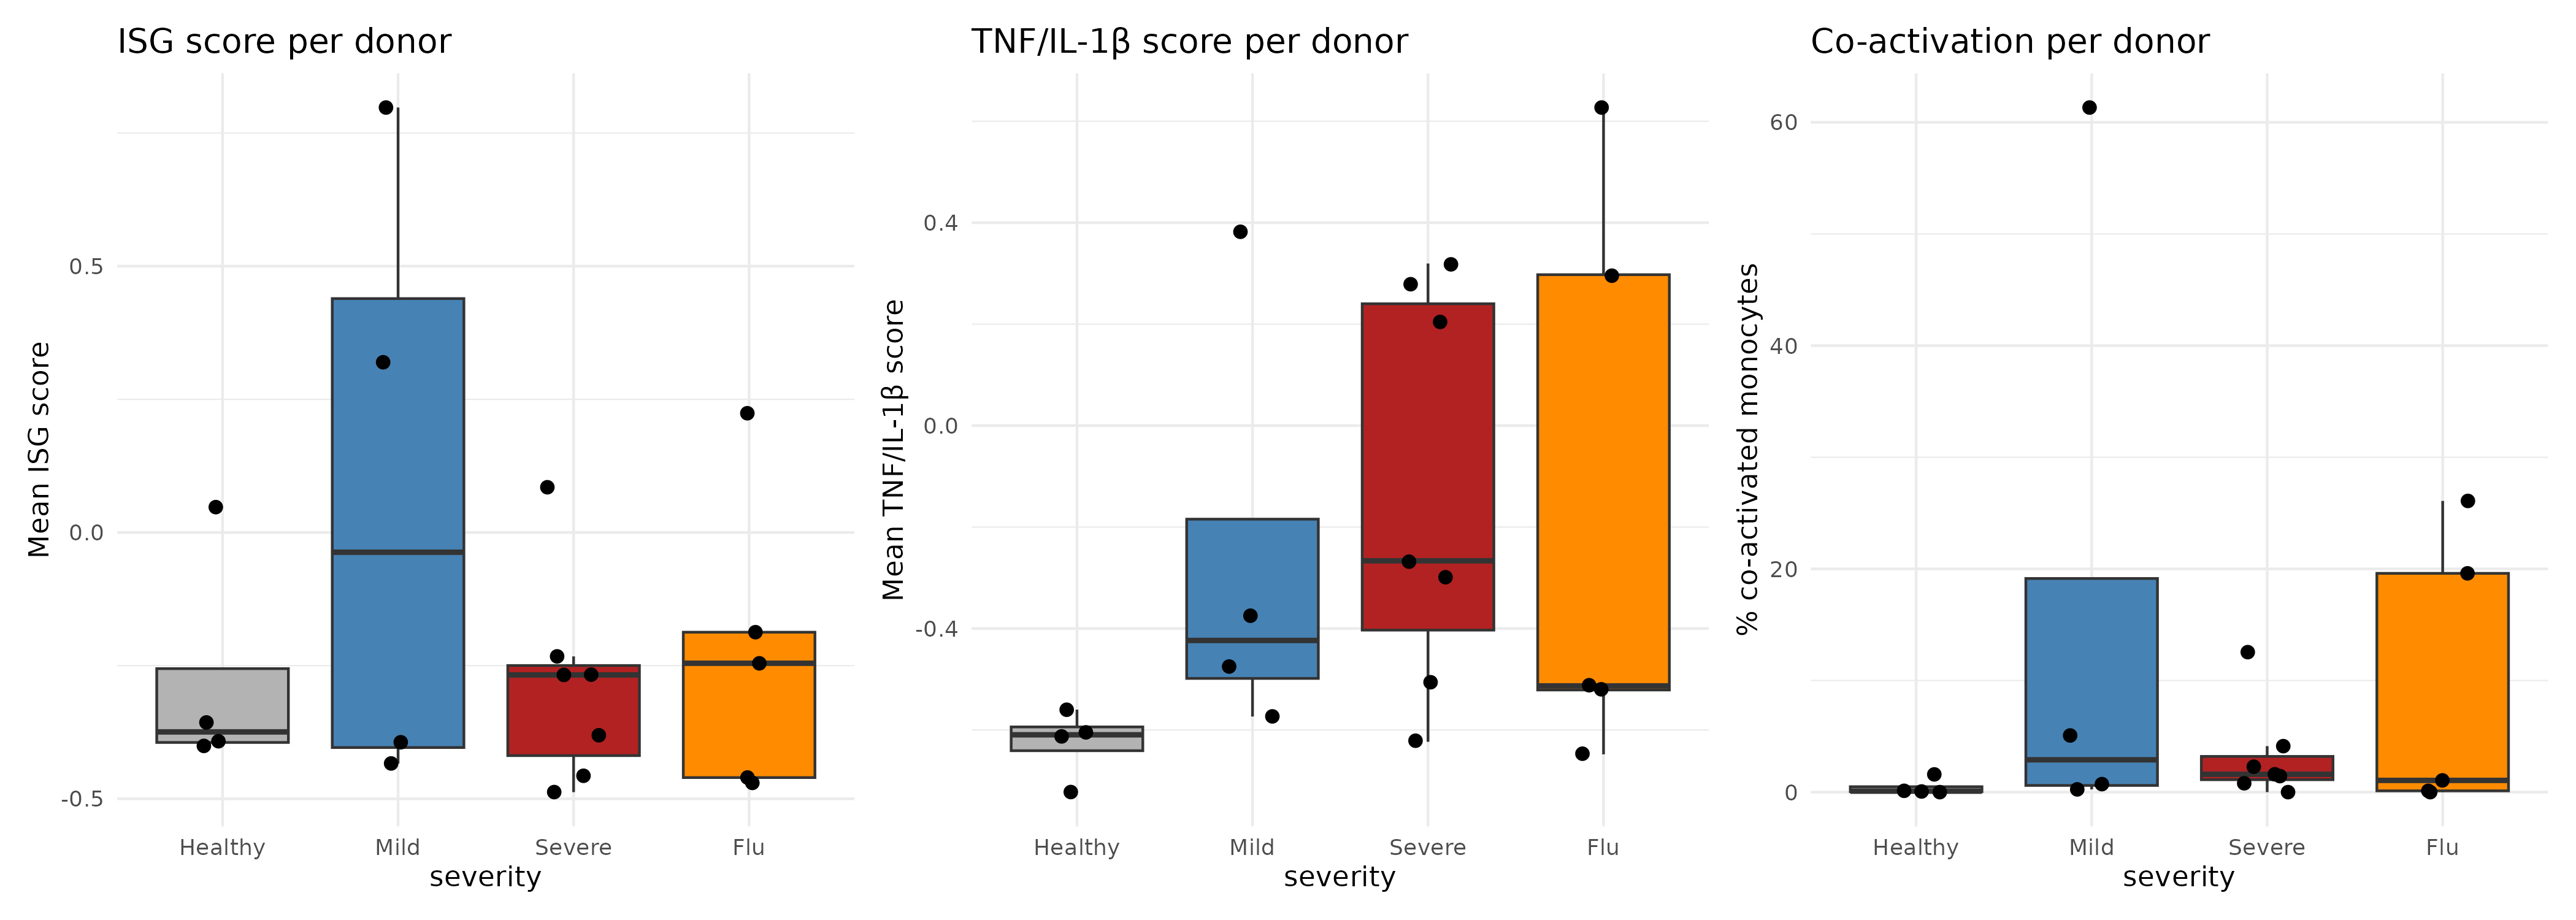
\includegraphics[width=\textwidth]{plots/phase4/phase4_donor_boxplots.png}
\end{center}

Each dot is one donor:
\begin{itemize}[nosep]
  \item \textbf{ISG score}: Mild COVID donors have the highest median — the antiviral program peaks in mild, not severe, disease.
  \item \textbf{TNF/IL-1$\beta$ score}: Severe and Flu donors are clearly elevated above Healthy. The inflammatory program tracks with disease severity.
  \item \textbf{Co-activation \%}: Healthy donors have $\sim$0\%. One Severe donor reaches 61\% co-activation — an extraordinary rate. Within-group variance is high, reflecting genuine donor heterogeneity.
\end{itemize}

With only 4--7 donors per group, formal Wilcoxon tests lack power, but the
directional trends are consistent across all analyses.

\subsection{Differential expression: Severe vs Healthy monocytes}

\texttt{FindMarkers} identified \textbf{3,269 DE genes} between Severe and Healthy
monocytes (Wilcoxon test, $p_{\text{adj}} < 0.05$).

\begin{center}
  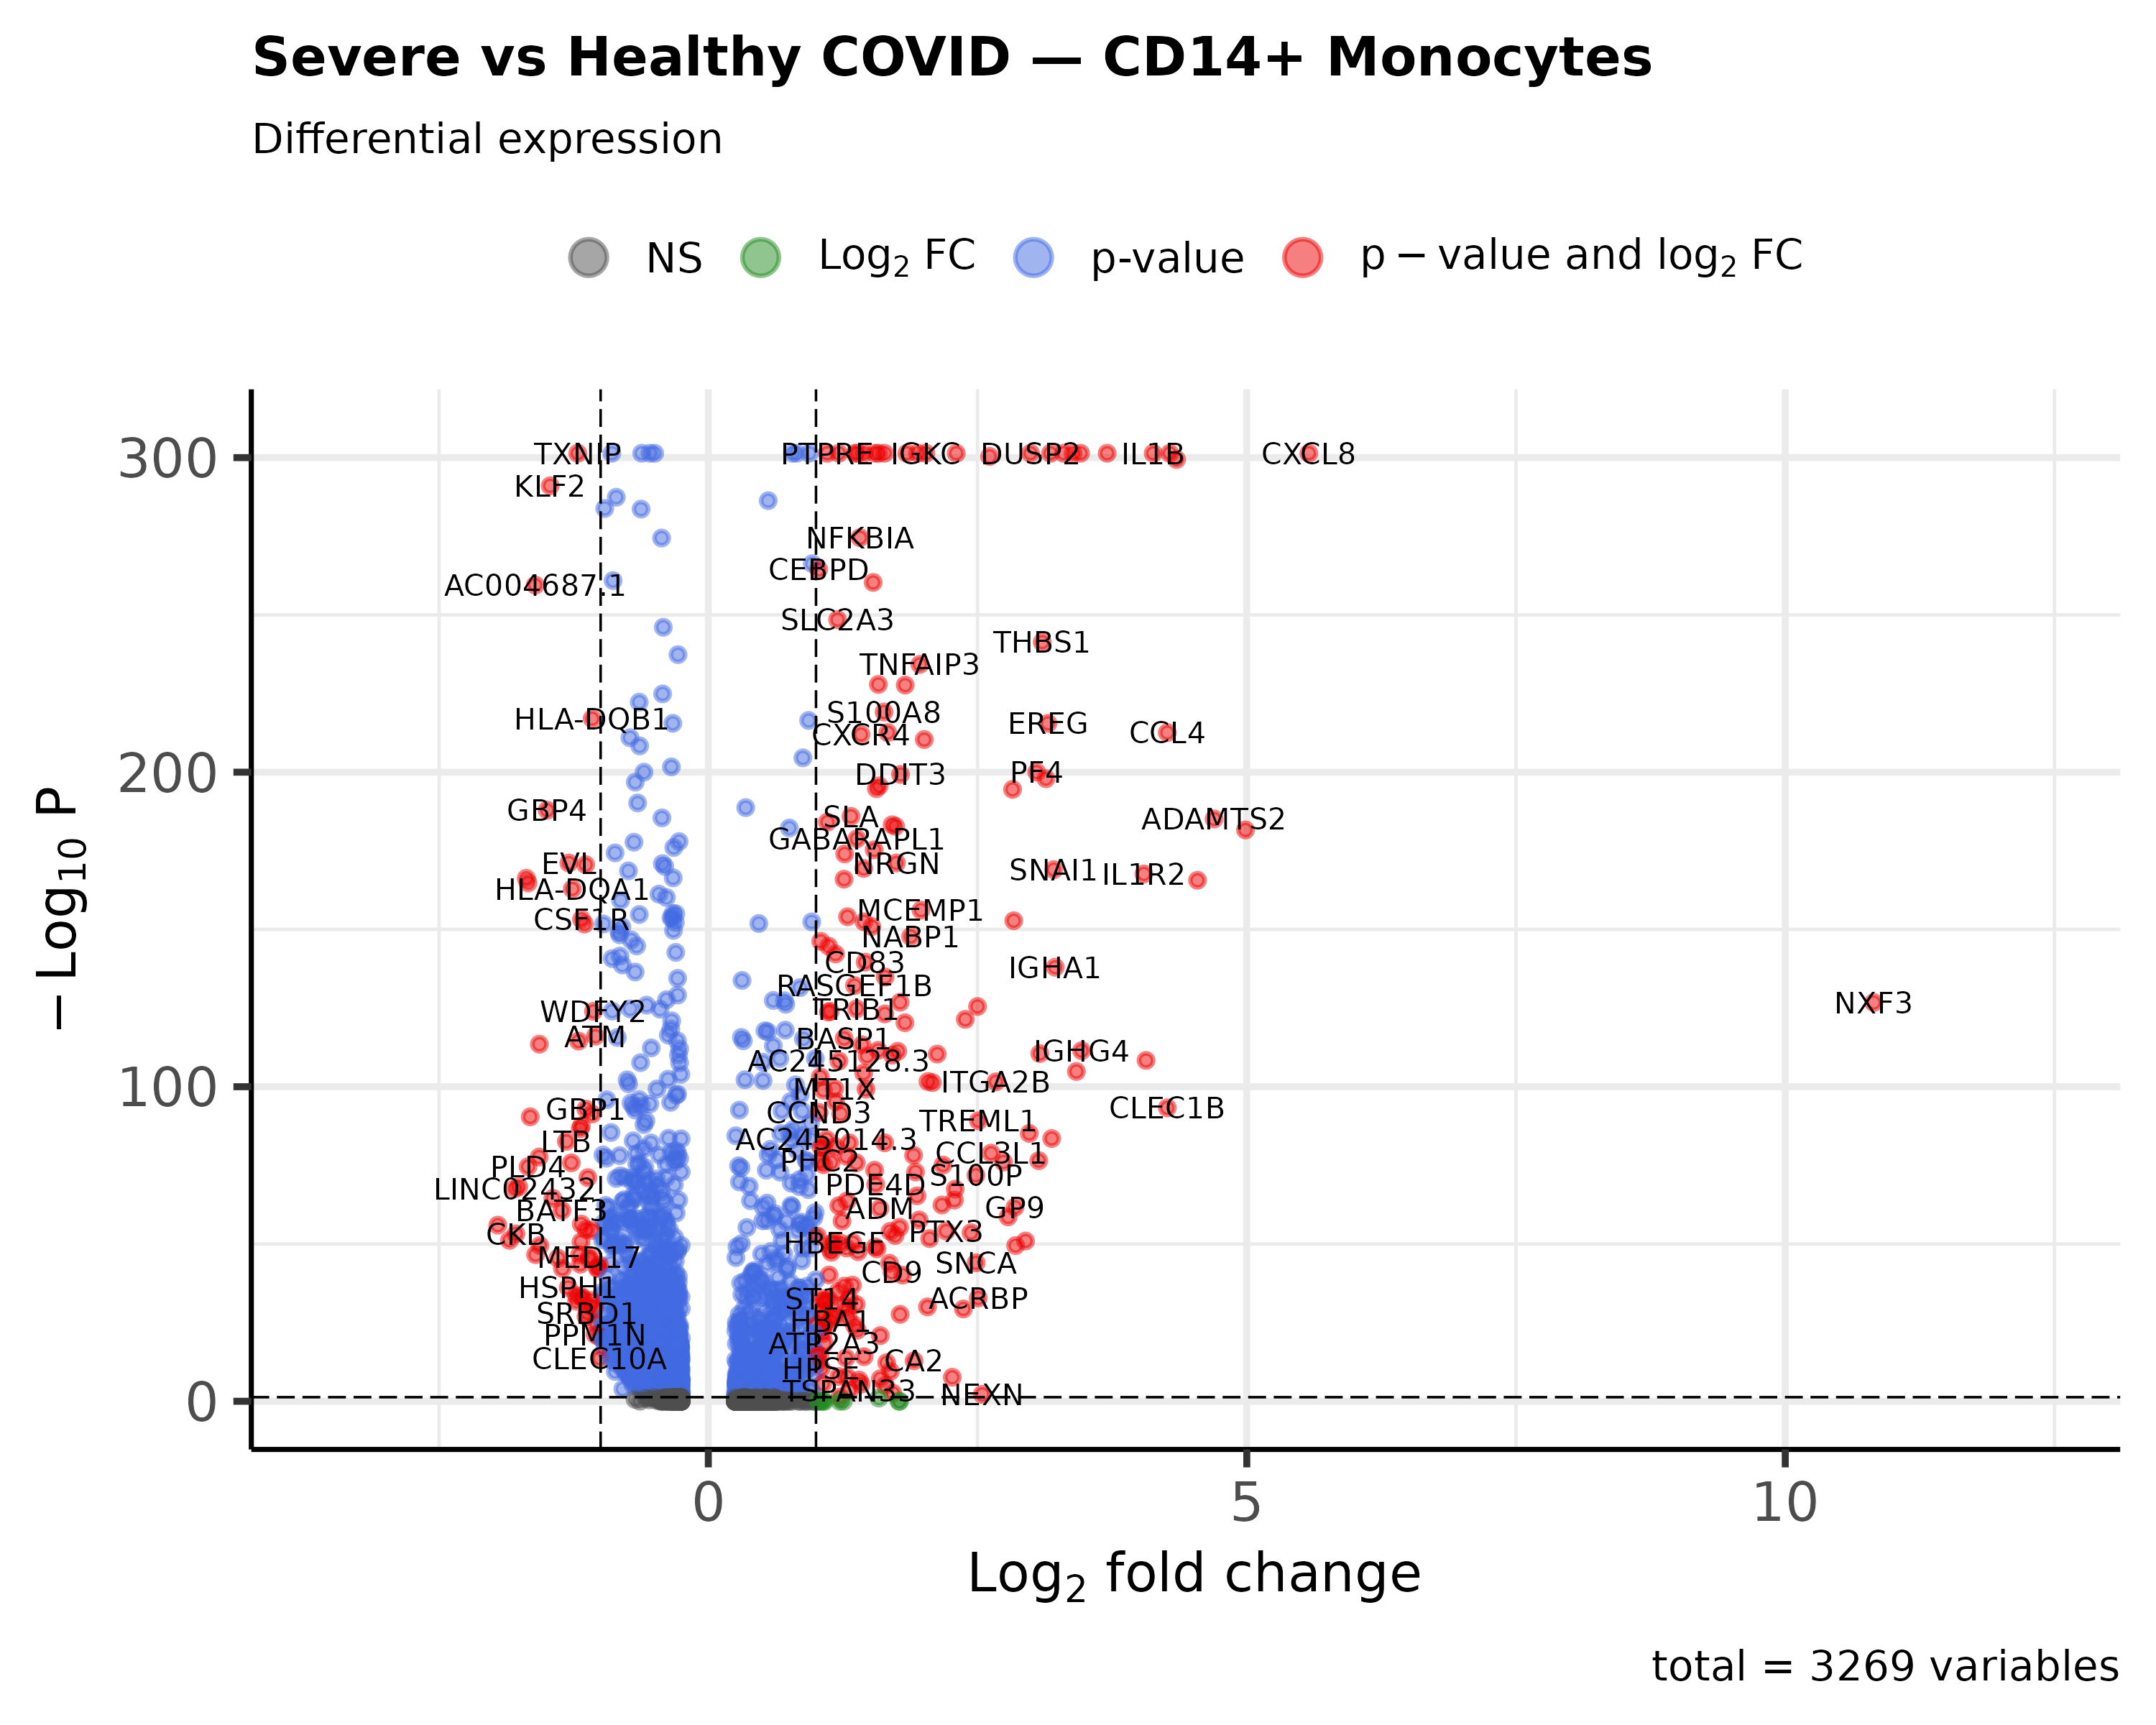
\includegraphics[width=0.95\textwidth]{plots/phase4/phase4_volcano_monocyte_DE.png}
\end{center}

The volcano plot reveals a pathological reprogramming:
\begin{itemize}[nosep]
  \item \textbf{Upregulated}: IL1B ($\log_2$FC $\approx 5$), CXCL8, CCL4, PTGS2 — the core inflammatory program. Also NFKBIA and TNFAIP3 (NF-$\kappa$B feedback inhibitors), indicating chronic activation.
  \item \textbf{Downregulated}: HLA-DQA1, HLA-DQB1 (antigen presentation lost), KLF2 (homeostatic identity lost), TXNIP (oxidative stress brake lost).
\end{itemize}

Severe COVID monocytes gain massive inflammatory output while simultaneously losing
their antigen-presenting capacity — a dual change known as \textbf{monocyte immunoparalysis}.

% ═══════════════════════════════════════════════
\section{Phase 5 — Independent Replication (GSE150861)}
% ═══════════════════════════════════════════════

\subsection{Dataset and processing}

GSE150861 contains PBMCs from \textbf{2 severe COVID-19 patients} treated with
\textbf{Tocilizumab} (anti-IL-6R), sampled at \textbf{Day 1, Day 5, and Day 7}.
The exact same pipeline was applied: QC filtering, LogNormalize, 20 PCs, resolution 0.5,
SingleR annotation — with no parameter changes.

\begin{center}
  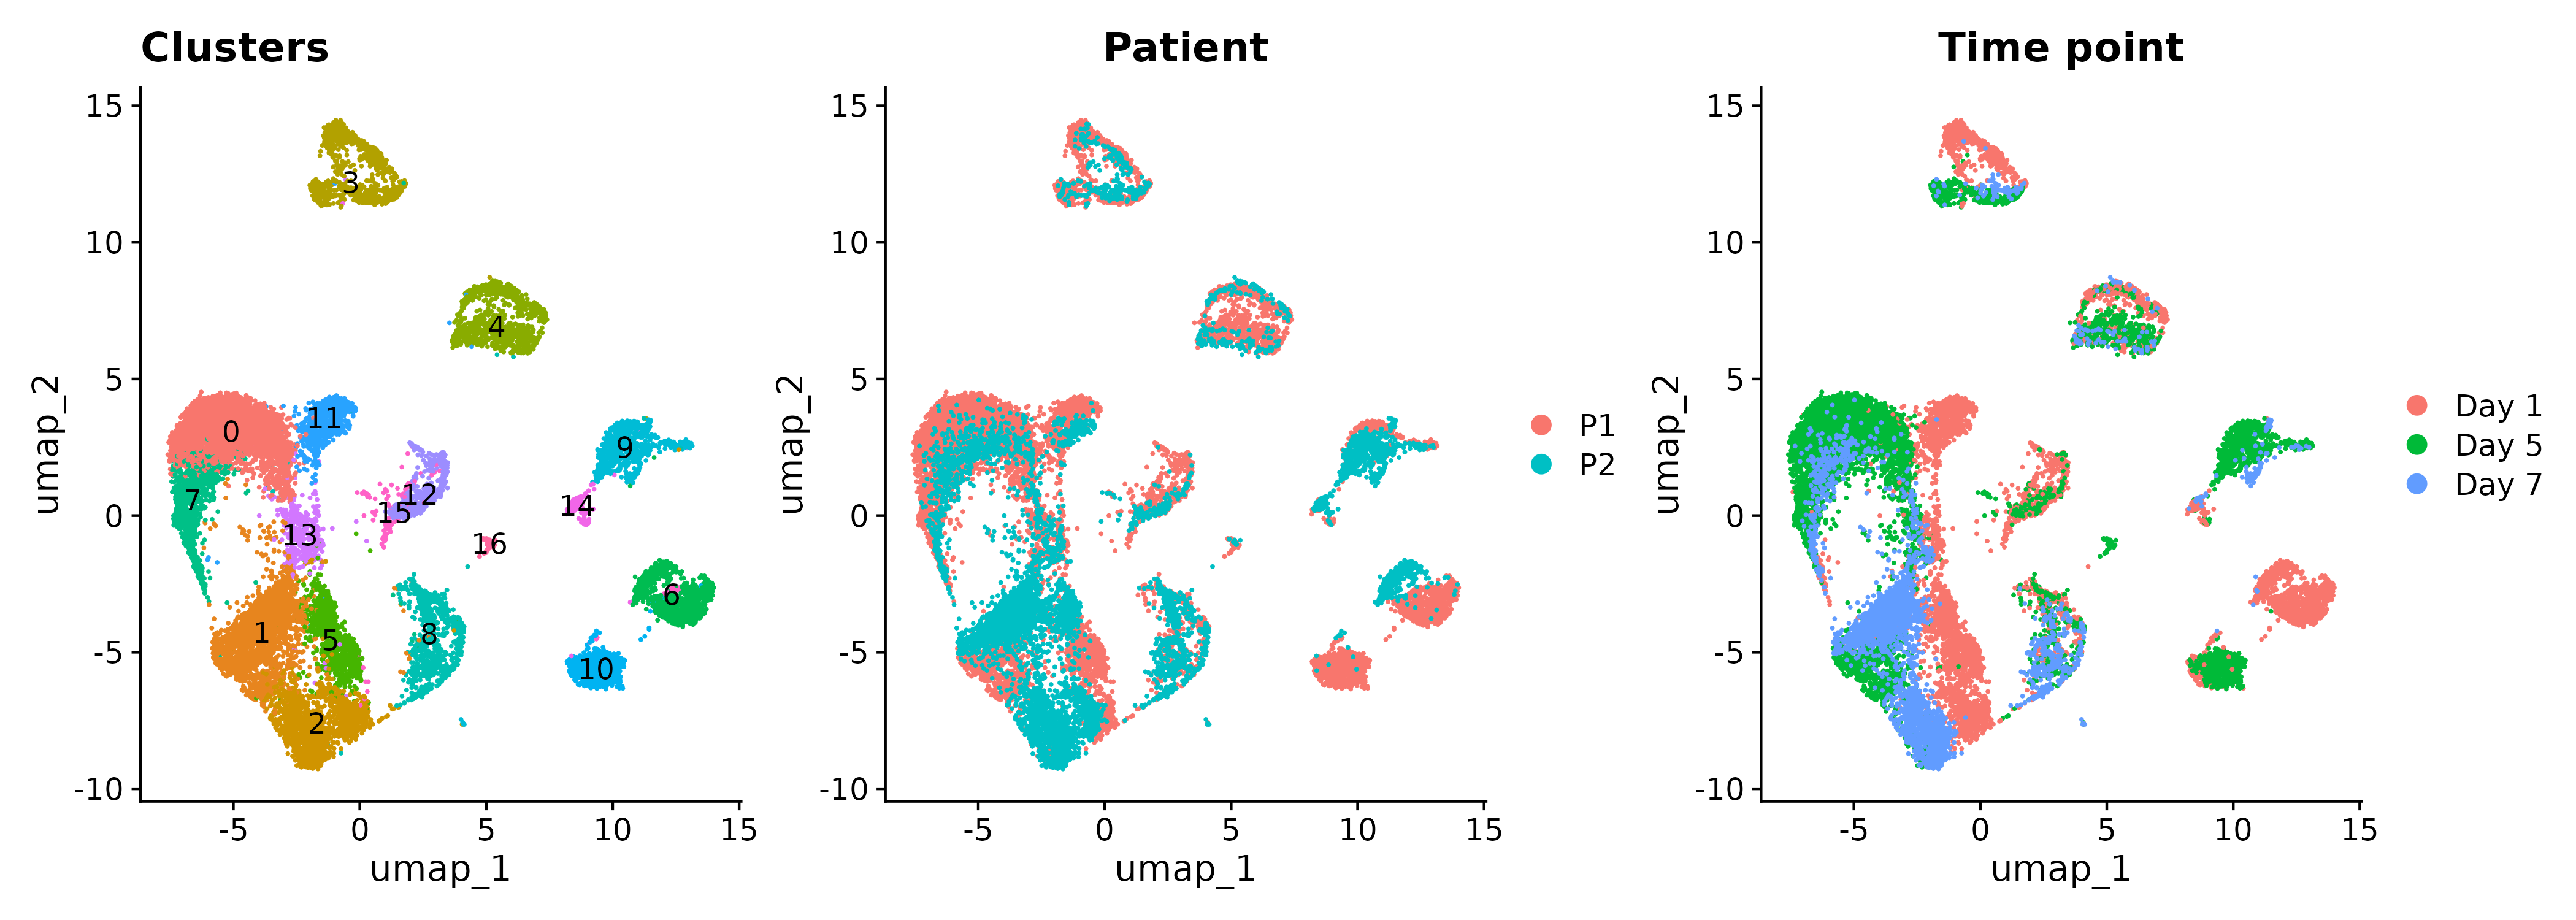
\includegraphics[width=\textwidth]{plots/phase5/phase5_umap_overview.png}
\end{center}

The UMAP shows 17 clusters with the same topology as the primary dataset
(lymphoid continent left, monocyte mass right, isolated B cell islands).
Critically, the patient-coloured panel shows P1 and P2 are \textbf{well-mixed across
clusters} — no batch effect. The time-point panel reveals Day 1 cells dominate
the monocyte mass, which thins by Day 5/7 under Tocilizumab treatment.

\subsection{Co-activation replicates}

The same ISG and TNF/IL-1$\beta$ module scoring was applied to the subset of
$\sim$8,000 monocytes.

\begin{center}
  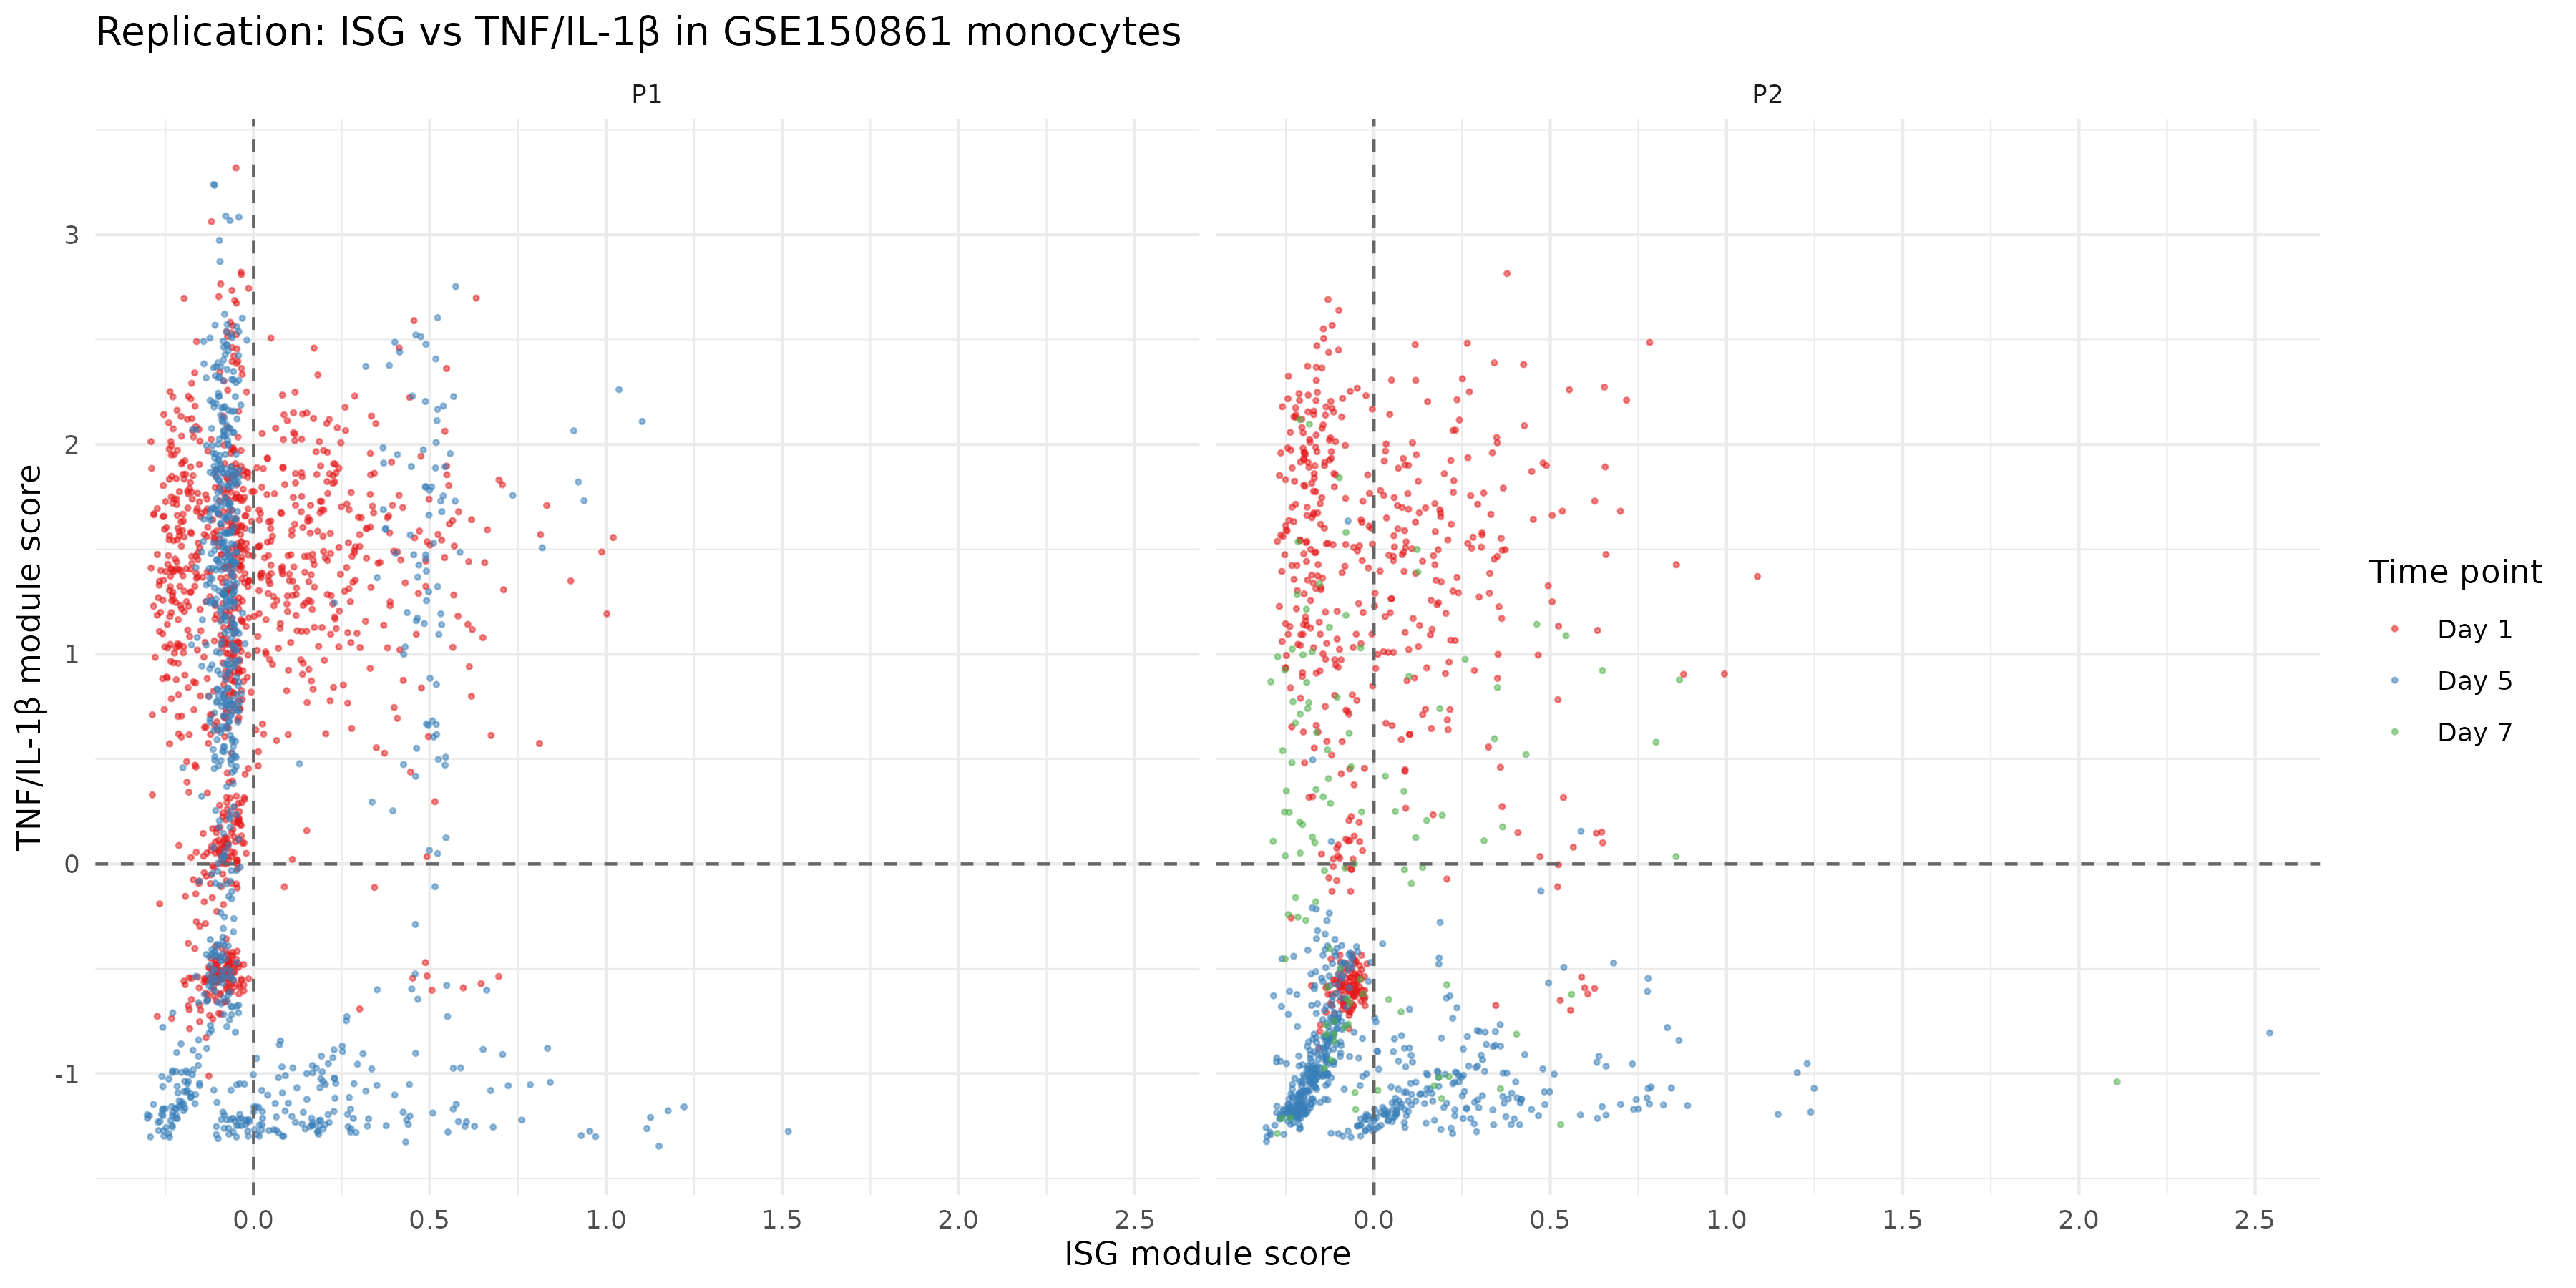
\includegraphics[width=\textwidth]{plots/phase5/phase5_coactivation_scatter.png}
\end{center}

\textbf{The co-activated state replicates.}
Day 1 cells (red) in both patients populate the top-right quadrant (co-activated)
and top-left (pure inflammation) — the same pattern as Severe COVID in Phase 4.
By Day 5 (blue), cells shift downward as Tocilizumab suppresses the inflammatory component.

\subsection{Longitudinal dynamics under Tocilizumab}

\begin{center}
  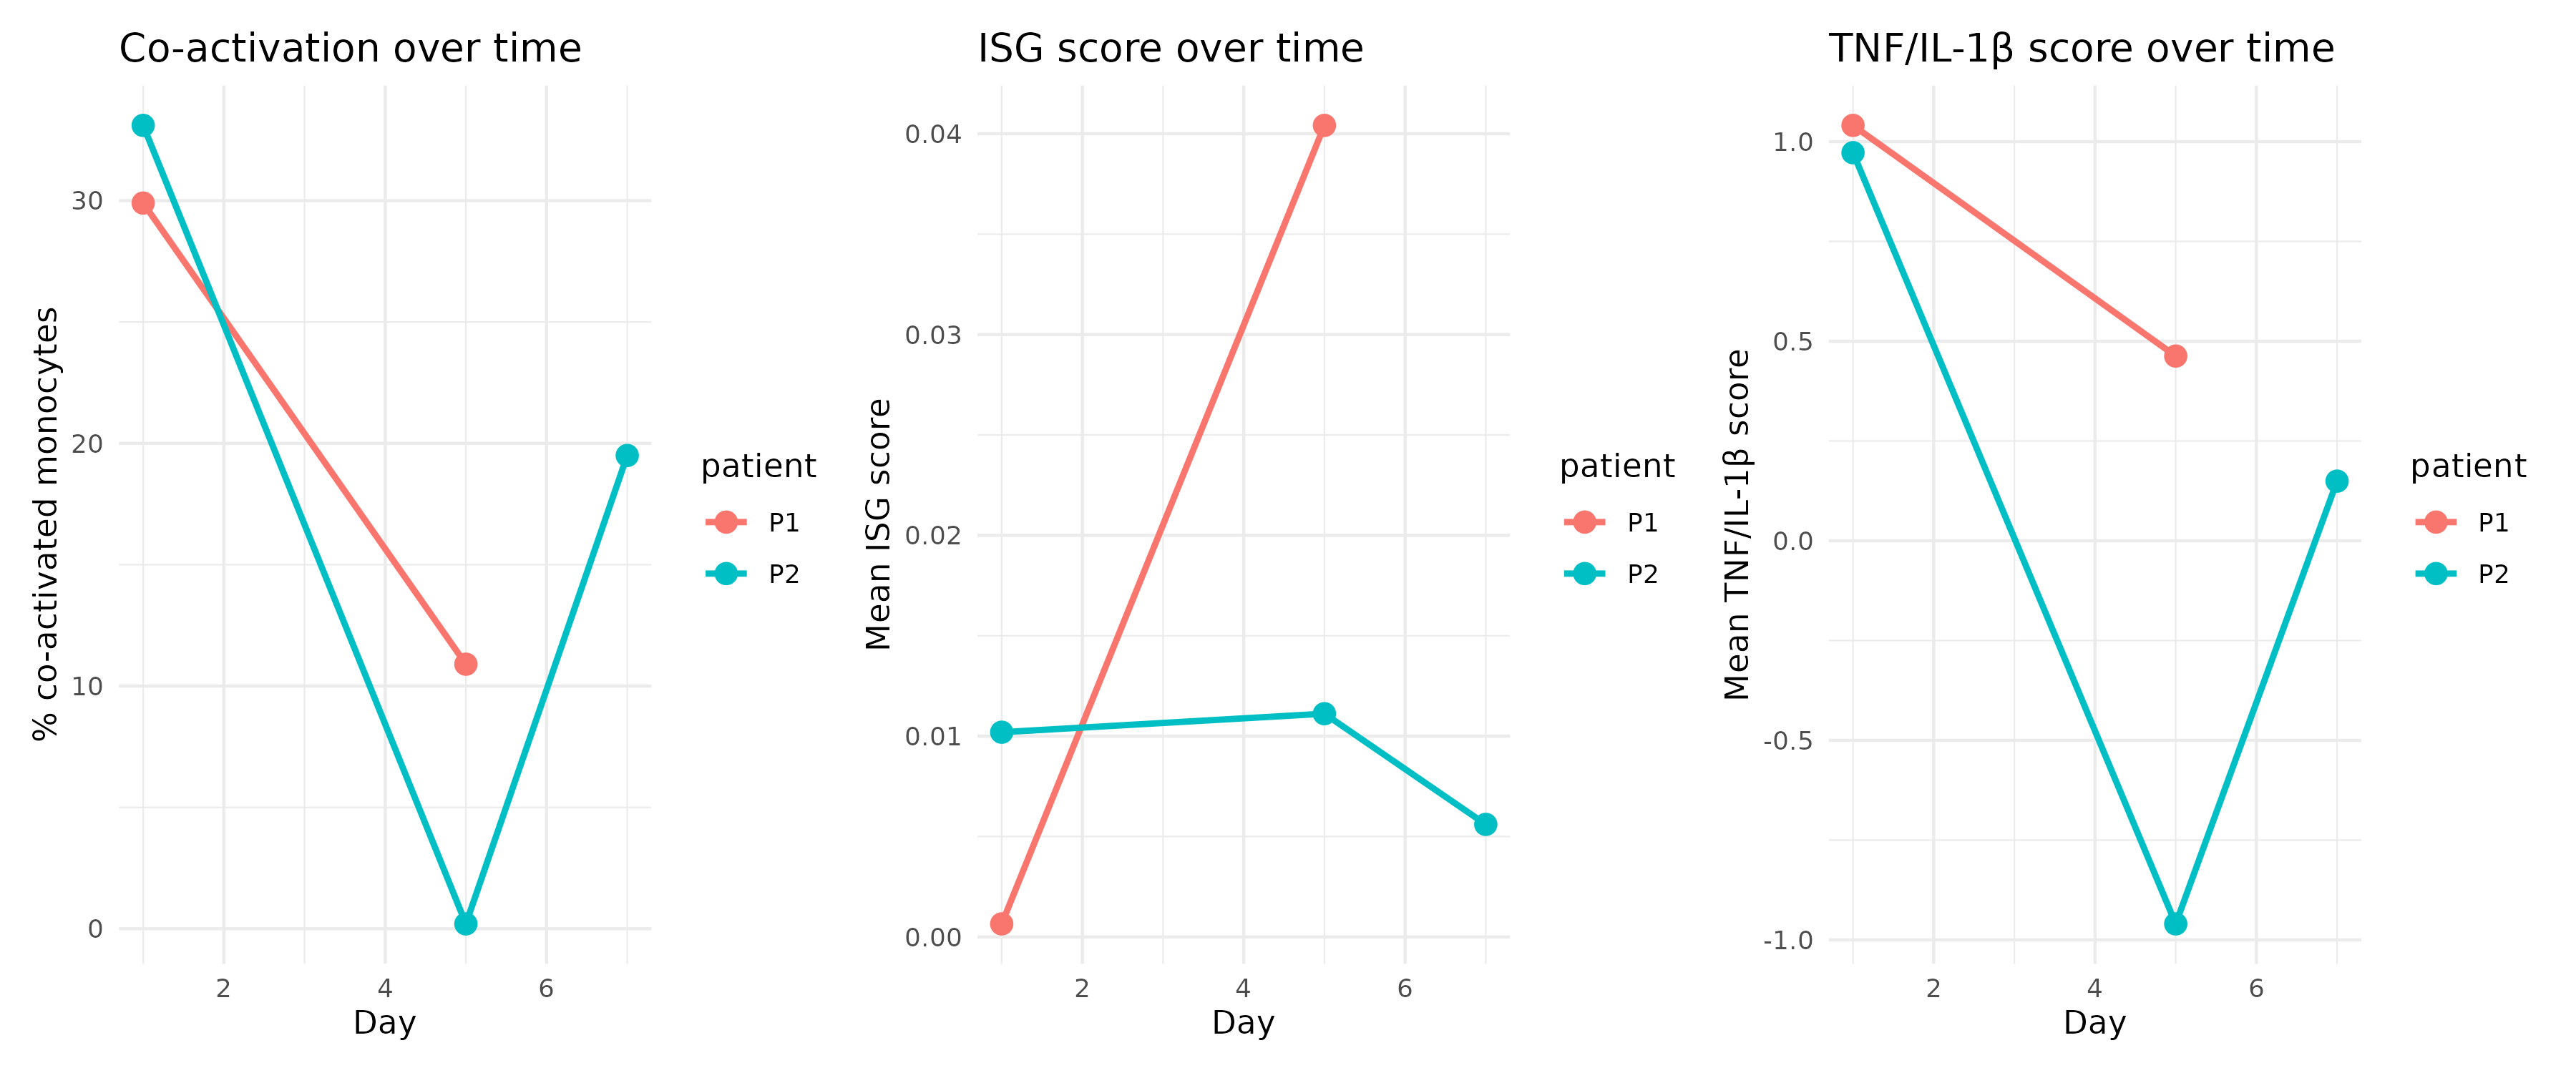
\includegraphics[width=\textwidth]{plots/phase5/phase5_longitudinal_dynamics.png}
\end{center}

Each point is one patient at one time point; lines connect the same patient across days.

\begin{itemize}[nosep]
  \item \textbf{Co-activation \% (left)}: Both patients start at $\sim$30--35\% on Day 1 — matching Phase 4 severe donors. By Day 5, both drop sharply. The consistent direction across both patients is the key result.
  \item \textbf{ISG score (middle)}: Stays near zero or slightly increases under treatment. Tocilizumab blocks IL-6, not interferons, so the antiviral program is unaffected.
  \item \textbf{TNF/IL-1$\beta$ score (right)}: Both patients start high ($\sim$+1.0) and drop sharply by Day 5. This is the clearest Tocilizumab signal — blocking IL-6R measurably reduces monocyte inflammatory output within 4 days.
\end{itemize}

The selective suppression of TNF/IL-1$\beta$ (but not ISG) under Tocilizumab
is biologically coherent and provides mechanistic evidence that the two programs
are independently regulated.

\textbf{Limitation}: with only 2 patients, no statistical test is meaningful.
The consistent direction across both patients is strong qualitative evidence
but cannot substitute for a larger cohort.

% ═══════════════════════════════════════════════
\section{Phase 6 — scRNA-seq Visualization Summary}
% ═══════════════════════════════════════════════

Before moving to bulk RNA-seq, we consolidate the single-cell findings into two summary
figures that frame the central paradox of what follows.

The composition barplot shows how the blood immune landscape changes with severity:

\begin{center}
  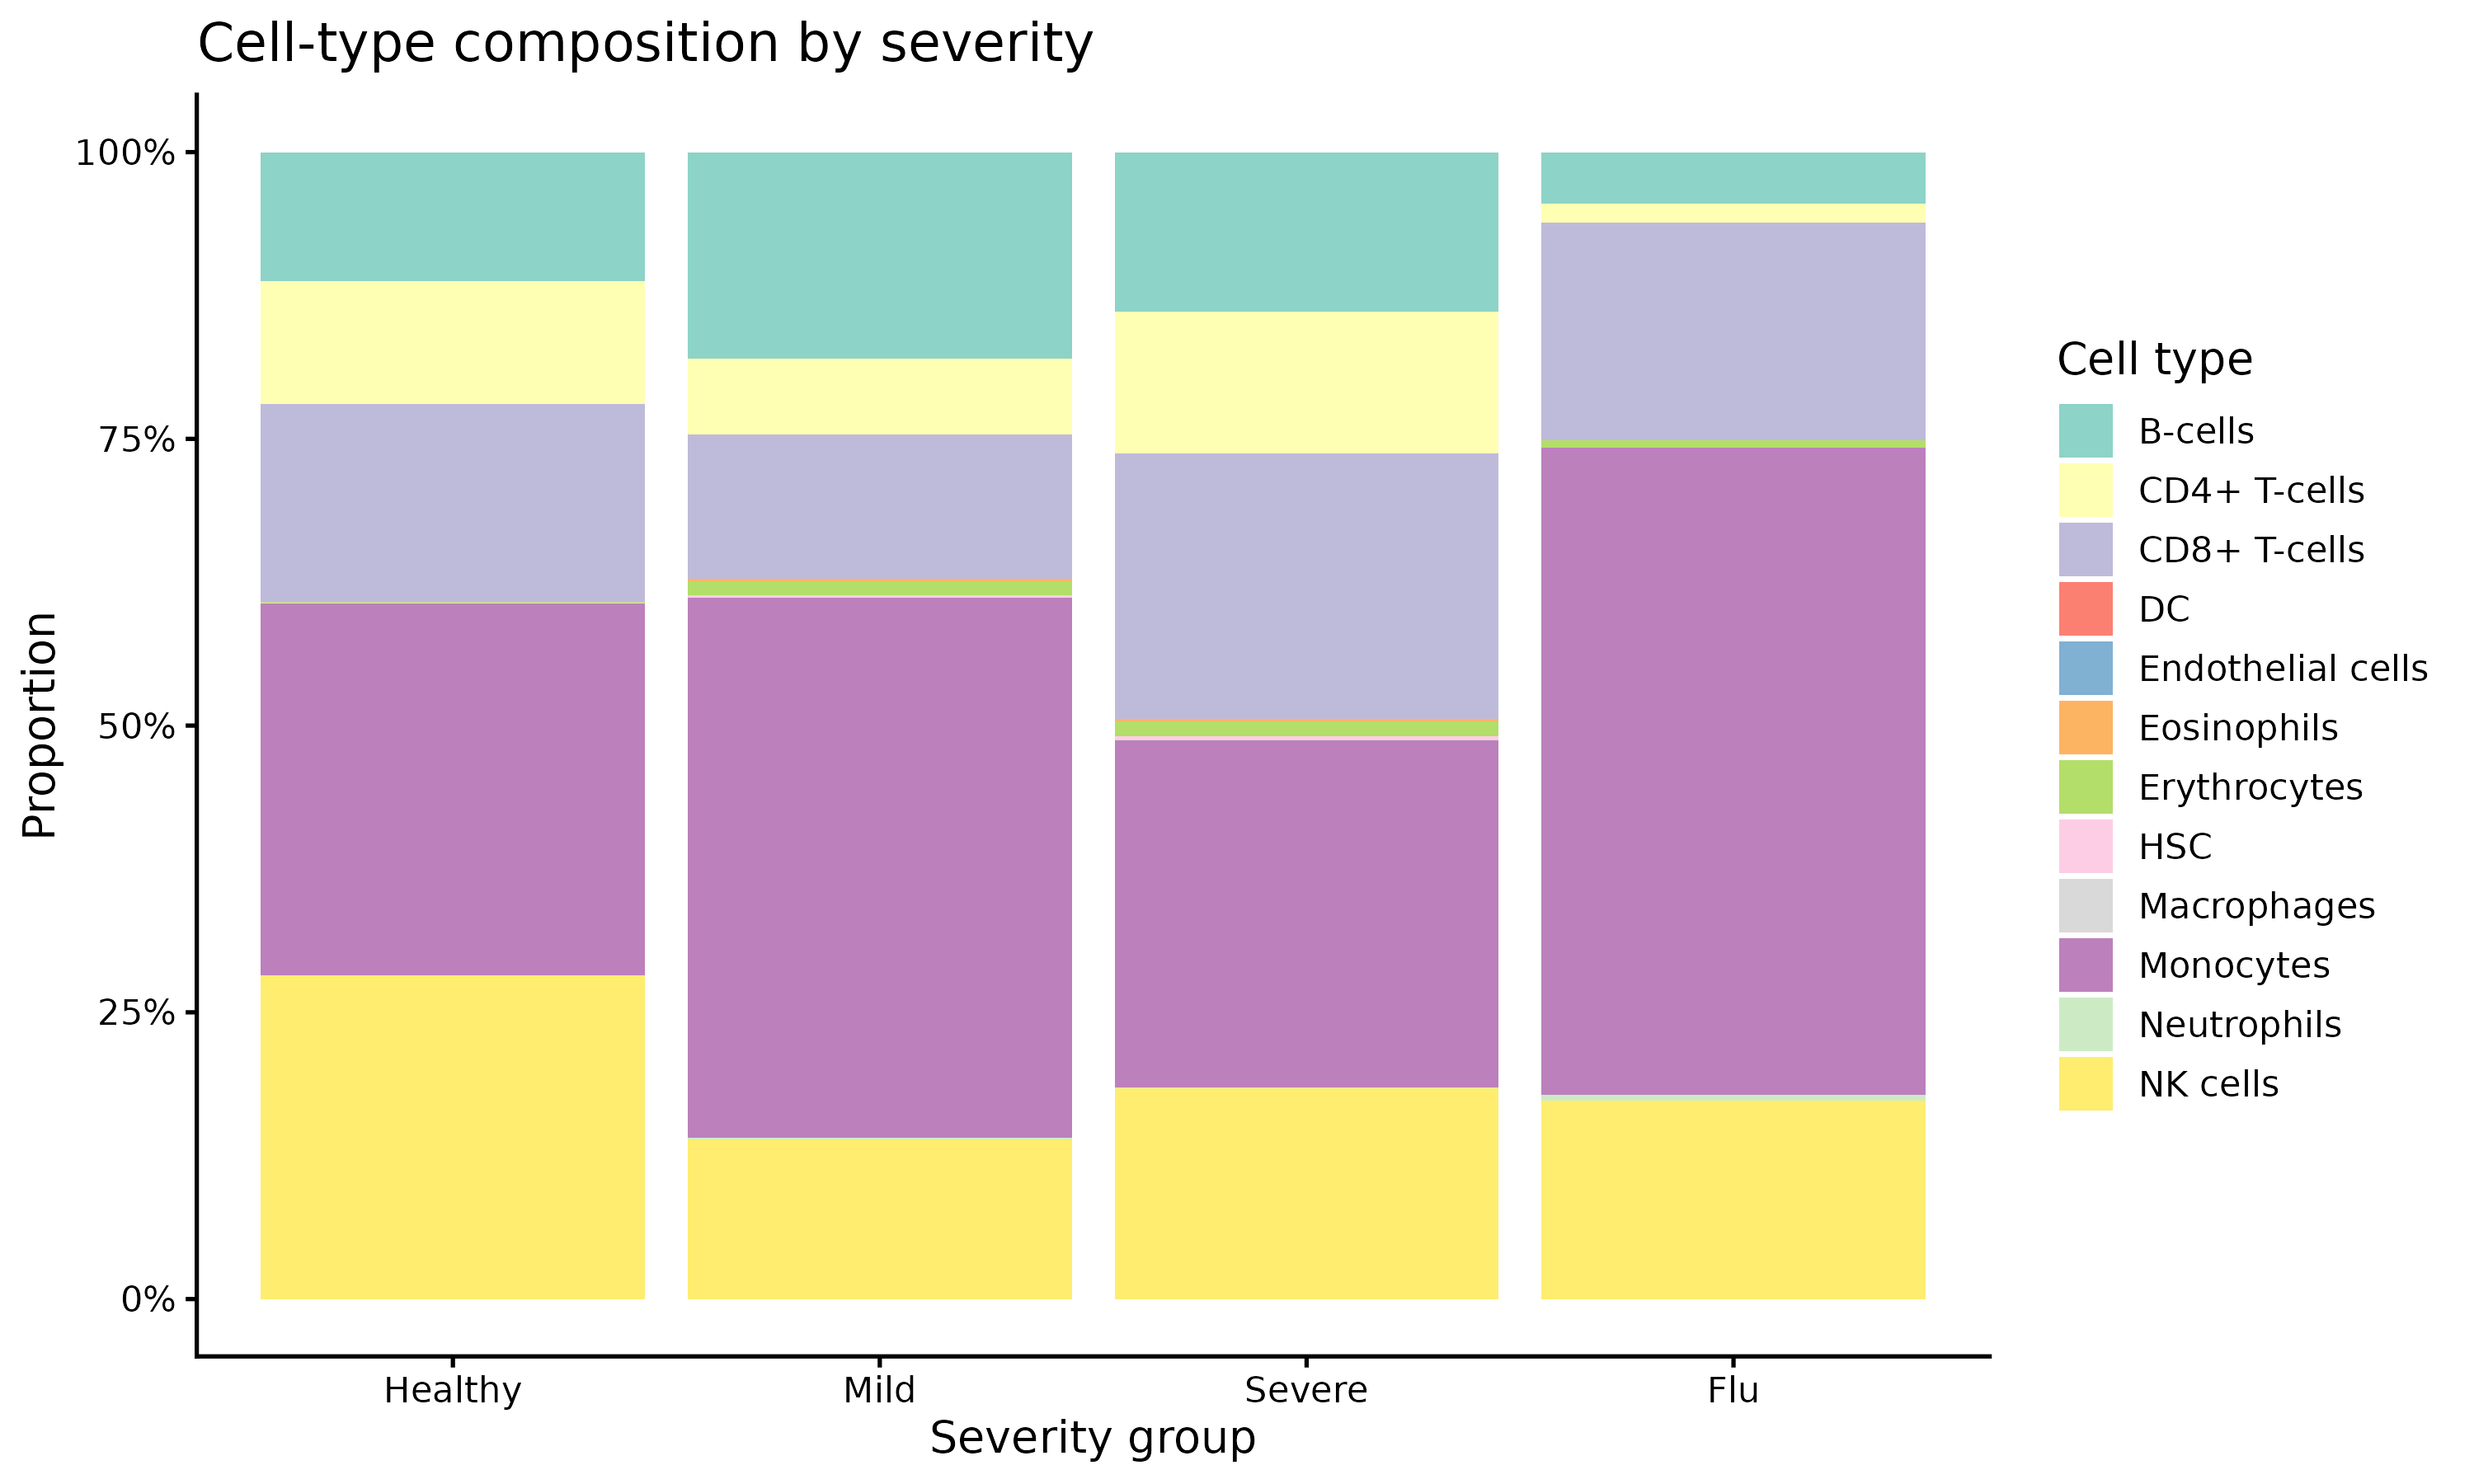
\includegraphics[width=0.85\textwidth]{plots/phase6/phase6_09_composition_barplot.png}
\end{center}

Monocytes rise from $\sim$35\% in Healthy to $\sim$50\% in Severe and $\sim$75\% in Flu.
NK and CD4$^+$ T cells are progressively lost. This cell-level shift is what makes bulk
RNA-seq difficult to interpret: when a monocyte-specific program goes up but the lymphocytes
that also express those genes disappear, the bulk net change may be zero or even negative.

The donor co-activation boxplot completes the picture:

\begin{center}
  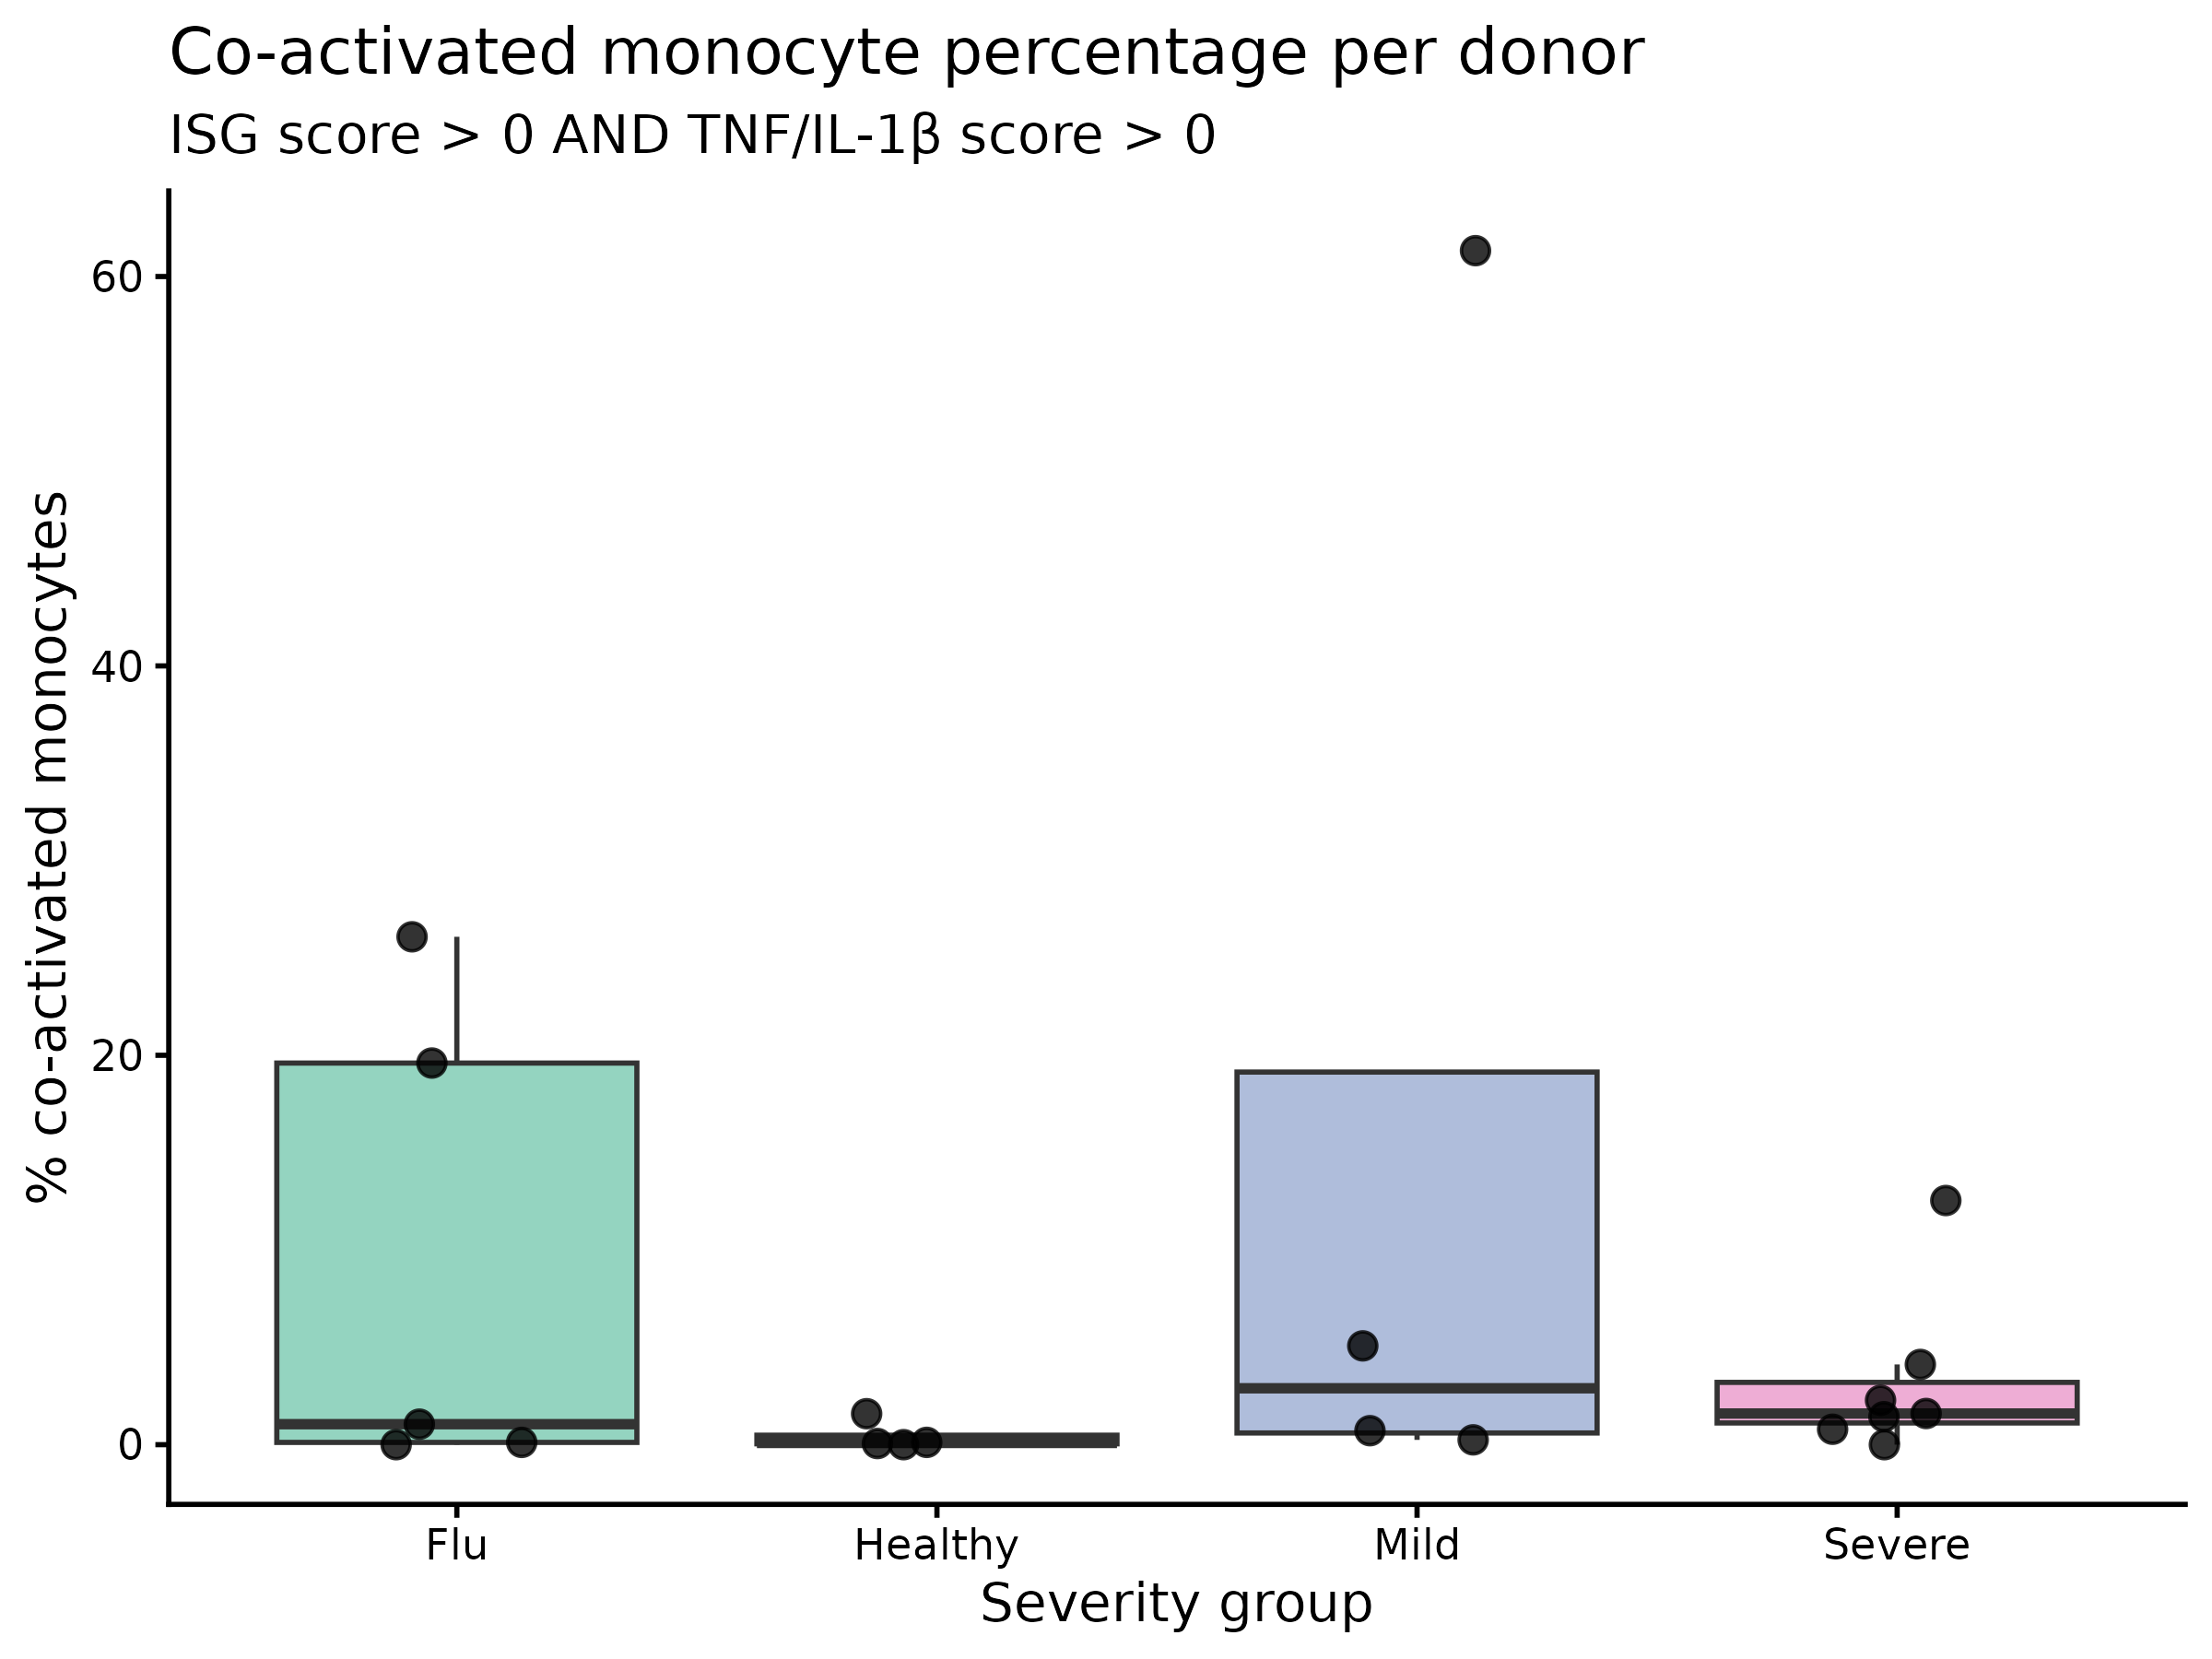
\includegraphics[width=0.85\textwidth]{plots/phase6/phase6_06_donor_coactivation_boxplot.png}
\end{center}

Flu has the highest co-activation, while Severe COVID monocytes are strongly inflammatory
but show \textit{lower} ISG co-activation than Mild — the two programs diverge as disease
worsens. This nuance is only visible at single-cell resolution, and we now ask whether any
trace of it survives averaging in bulk whole-blood data.

% ─────────────────────────────────
\bigskip
\noindent\textbf{The bulk chapter.}\quad
Phases 7--13 shift to \textbf{GSE152418} (Arunachalam et al., \textit{Science} 2020) —
33 whole-blood bulk RNA-seq samples from COVID-19 patients across severity levels.
Unlike scRNA-seq, bulk data averages expression across all cell types simultaneously,
making cell-type-specific programs harder to detect but providing more samples and
greater statistical power for detecting broad transcriptomic changes.

% ═══════════════════════════════════════════════
\section{Phase 7 — Bulk Data Loading and Exploratory Analysis}
% ═══════════════════════════════════════════════

Before any statistical test, we verified that the data is clean and that no technical
confounders will corrupt the results. The 33 samples were grouped as
\textbf{Healthy/Mild} (21 samples) vs \textbf{Severe/ICU} (12 samples);
Convalescent samples were excluded as they represent recovery, not active disease.

\begin{center}
  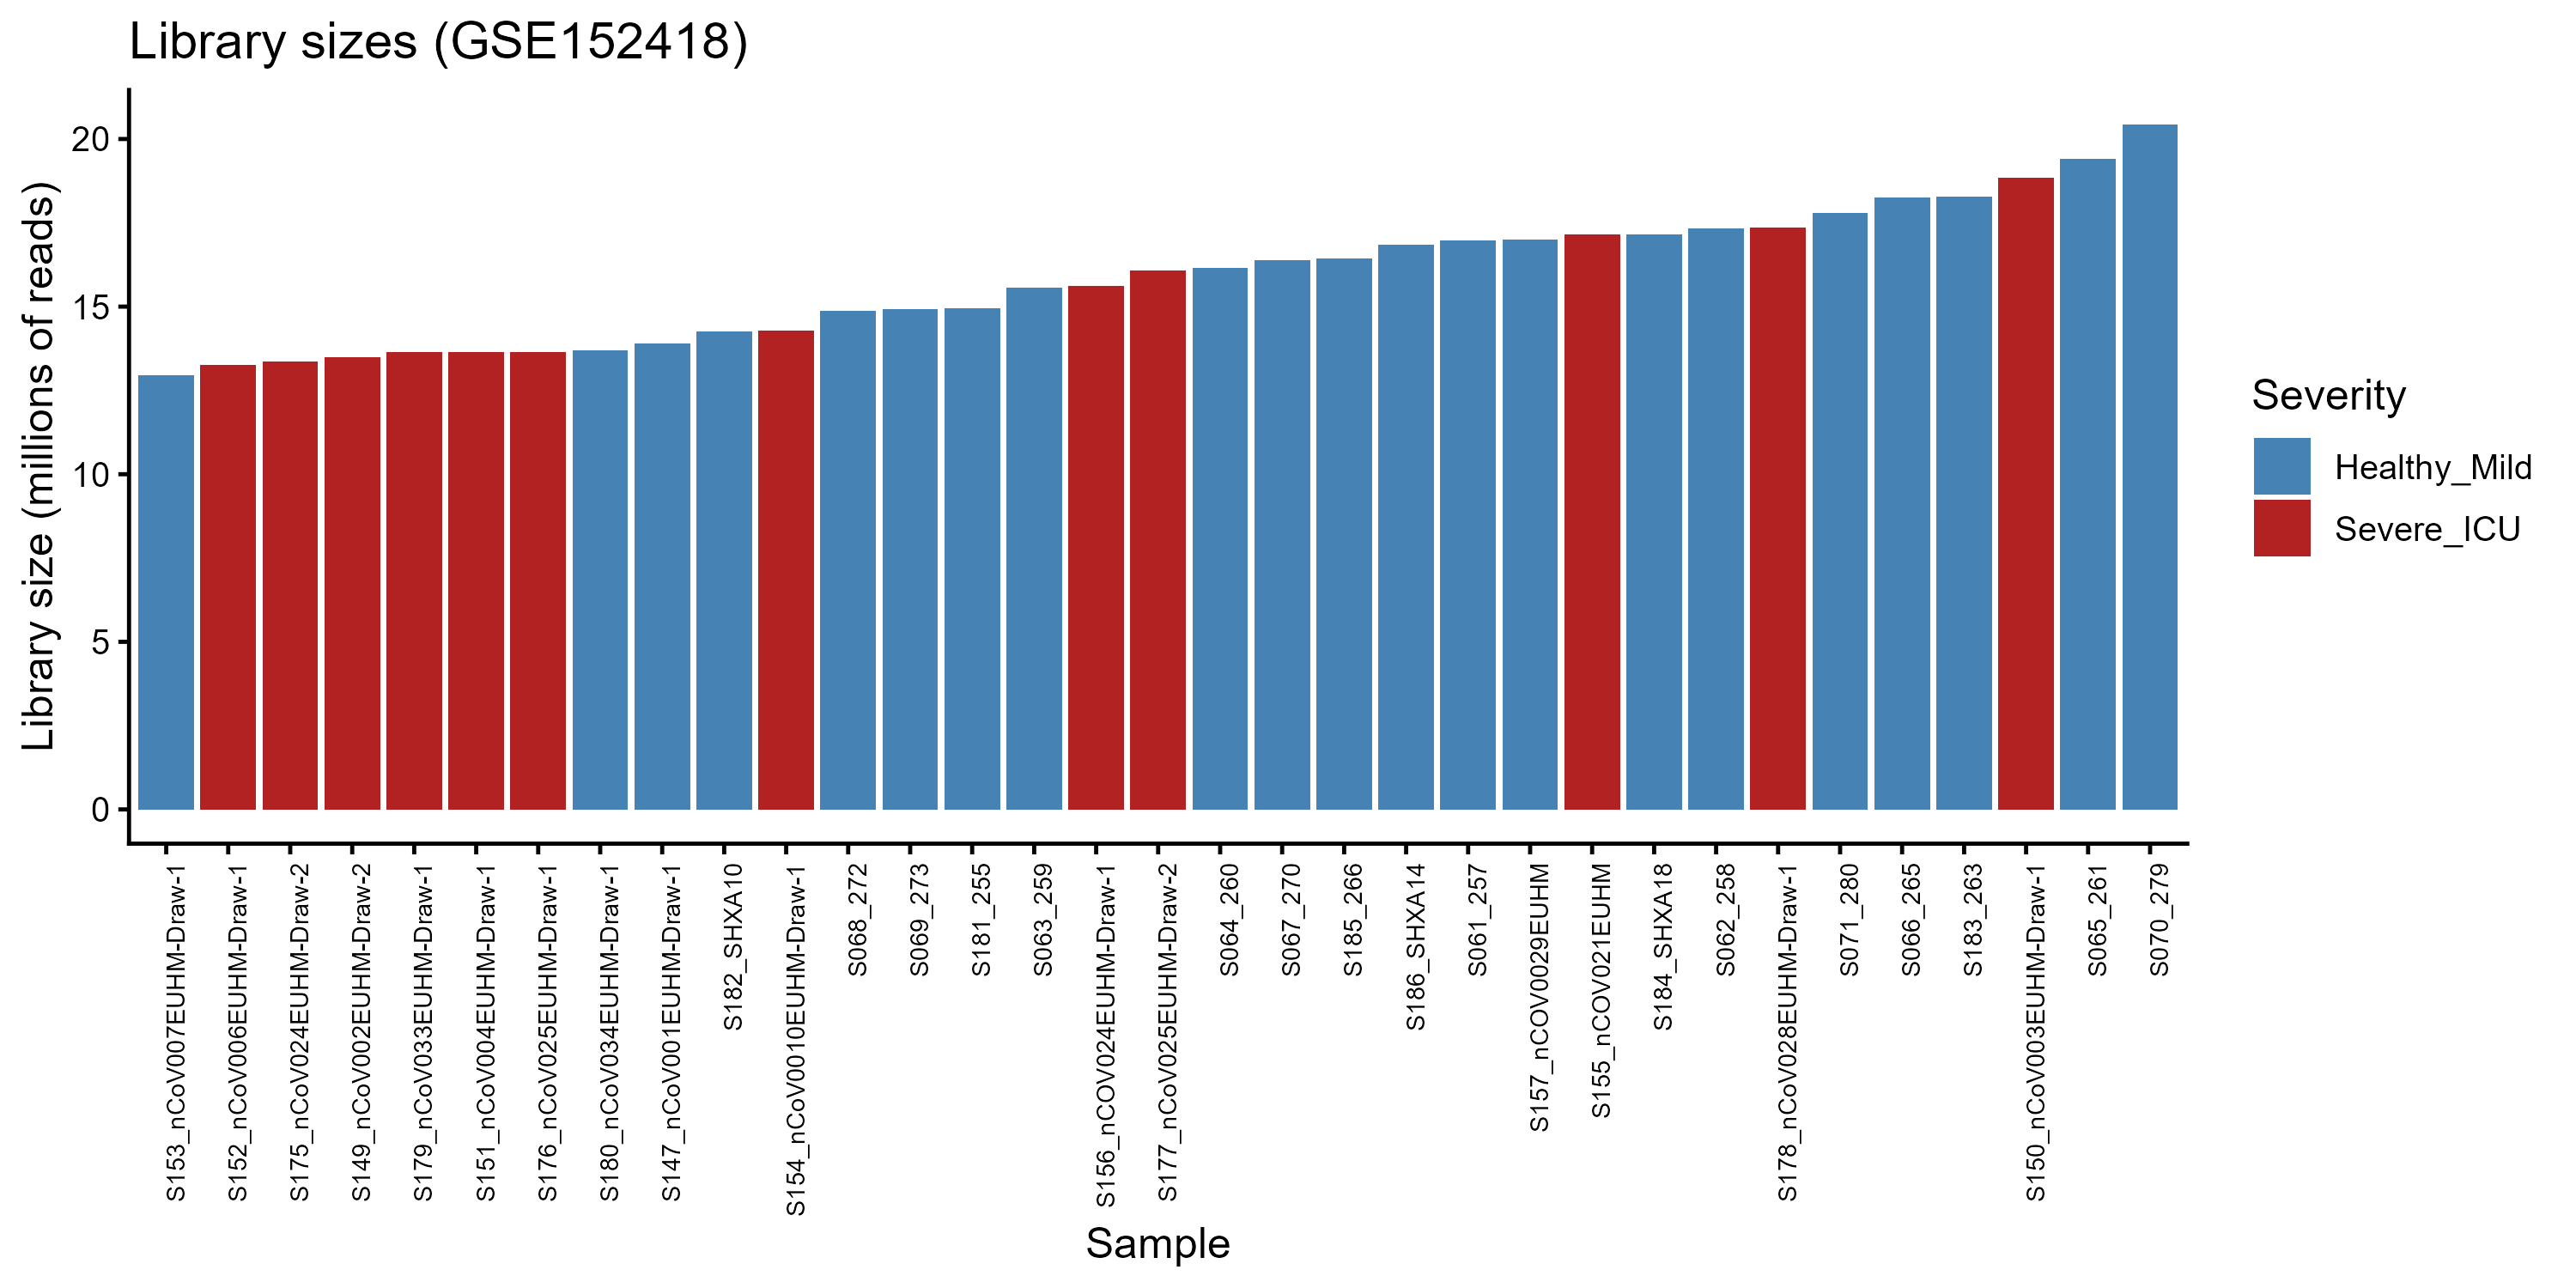
\includegraphics[width=\textwidth]{plots/phase7/phase7_library_sizes.png}
\end{center}

Library sizes range from 13M to 20M reads with red (Severe) and blue (Healthy) bars
fully intermixed — no depth bias between groups. DESeq2 size-factor normalization
handles the remaining $\sim$1.5$\times$ variation.

\begin{center}
  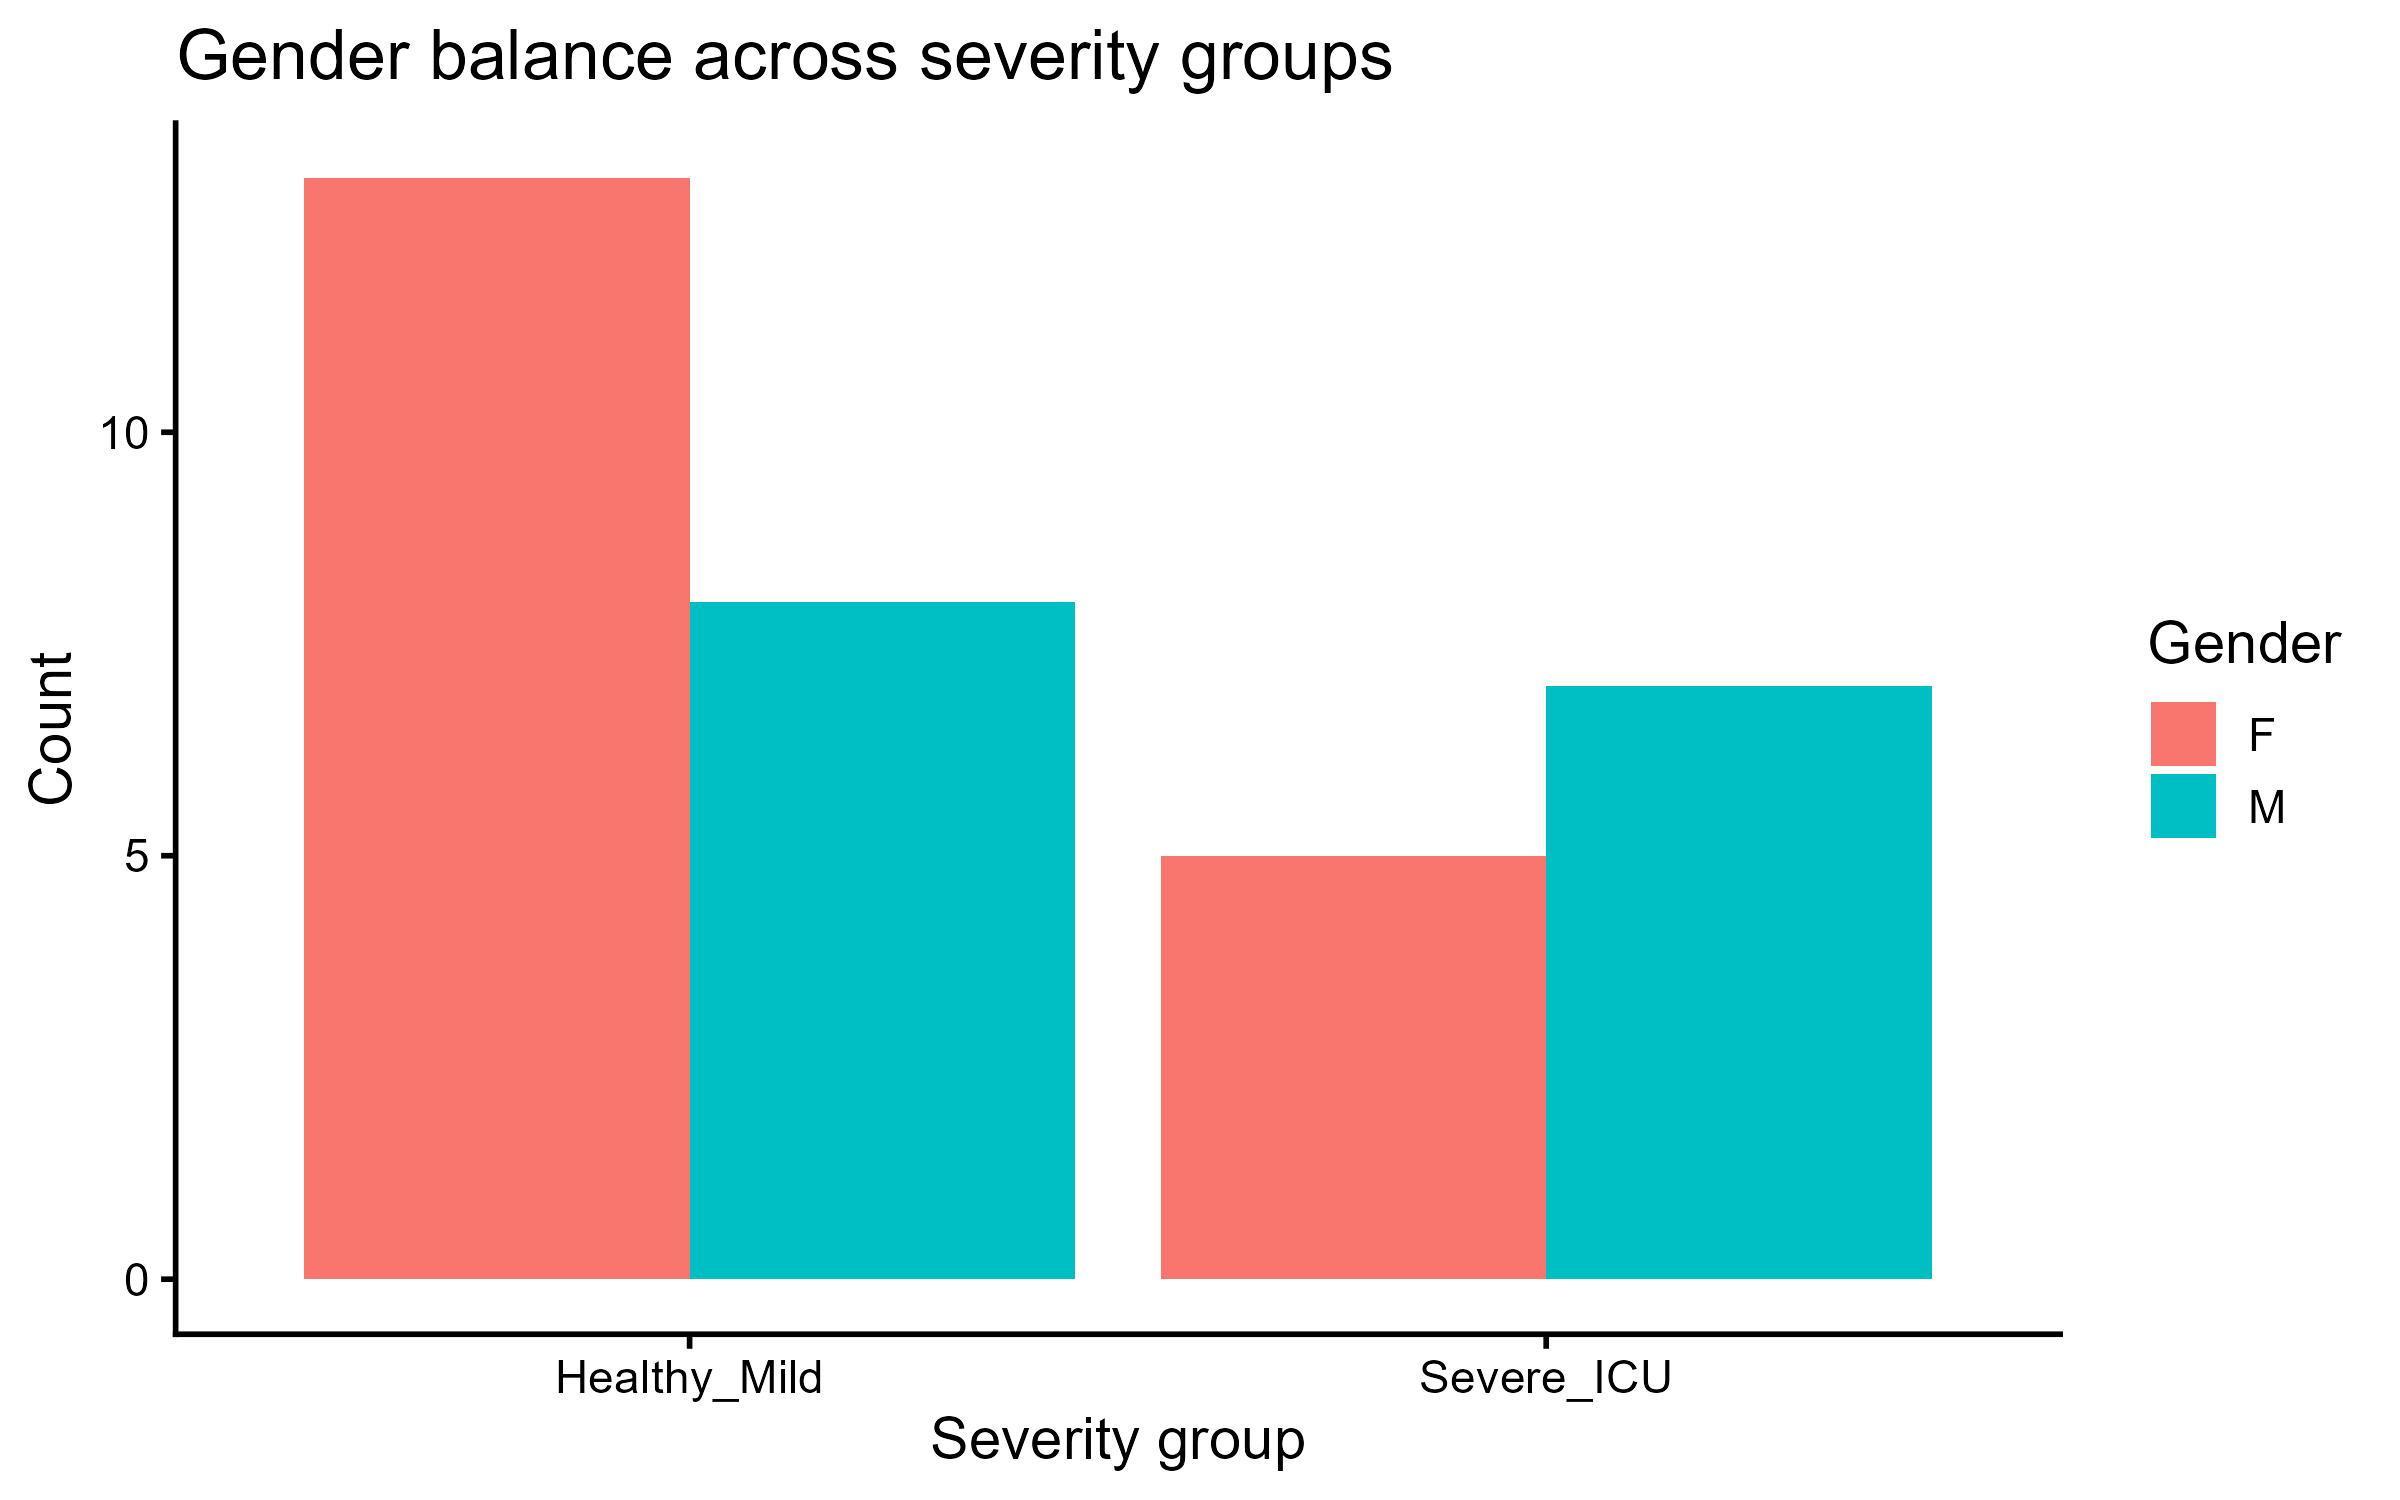
\includegraphics[width=0.72\textwidth]{plots/phase7/phase7_gender_balance.png}
\end{center}

A confounder emerged: Healthy/Mild is female-majority (13F/8M) while Severe/ICU is
male-majority (5F/7M). Since males have worse COVID outcomes on average, sex-biased
genes could masquerade as severity signals. This imbalance is flagged here and corrected
with an extended model in Phase 9.

% ═══════════════════════════════════════════════
\section{Phase 8 — DESeq2 Differential Expression}
% ═══════════════════════════════════════════════

With clean data in hand, we run the core statistical test: which genes are systematically
different in whole blood between Severe/ICU and Healthy/Mild?
DESeq2 is used rather than a t-test because RNA-seq counts are \textbf{overdispersed}
(variance $\gg$ mean) — the mean-variance plot confirmed this for every gene in the dataset.
DESeq2's negative binomial model and apeglm fold-change shrinkage give reliable,
conservative estimates even for lowly expressed genes.

\begin{center}
  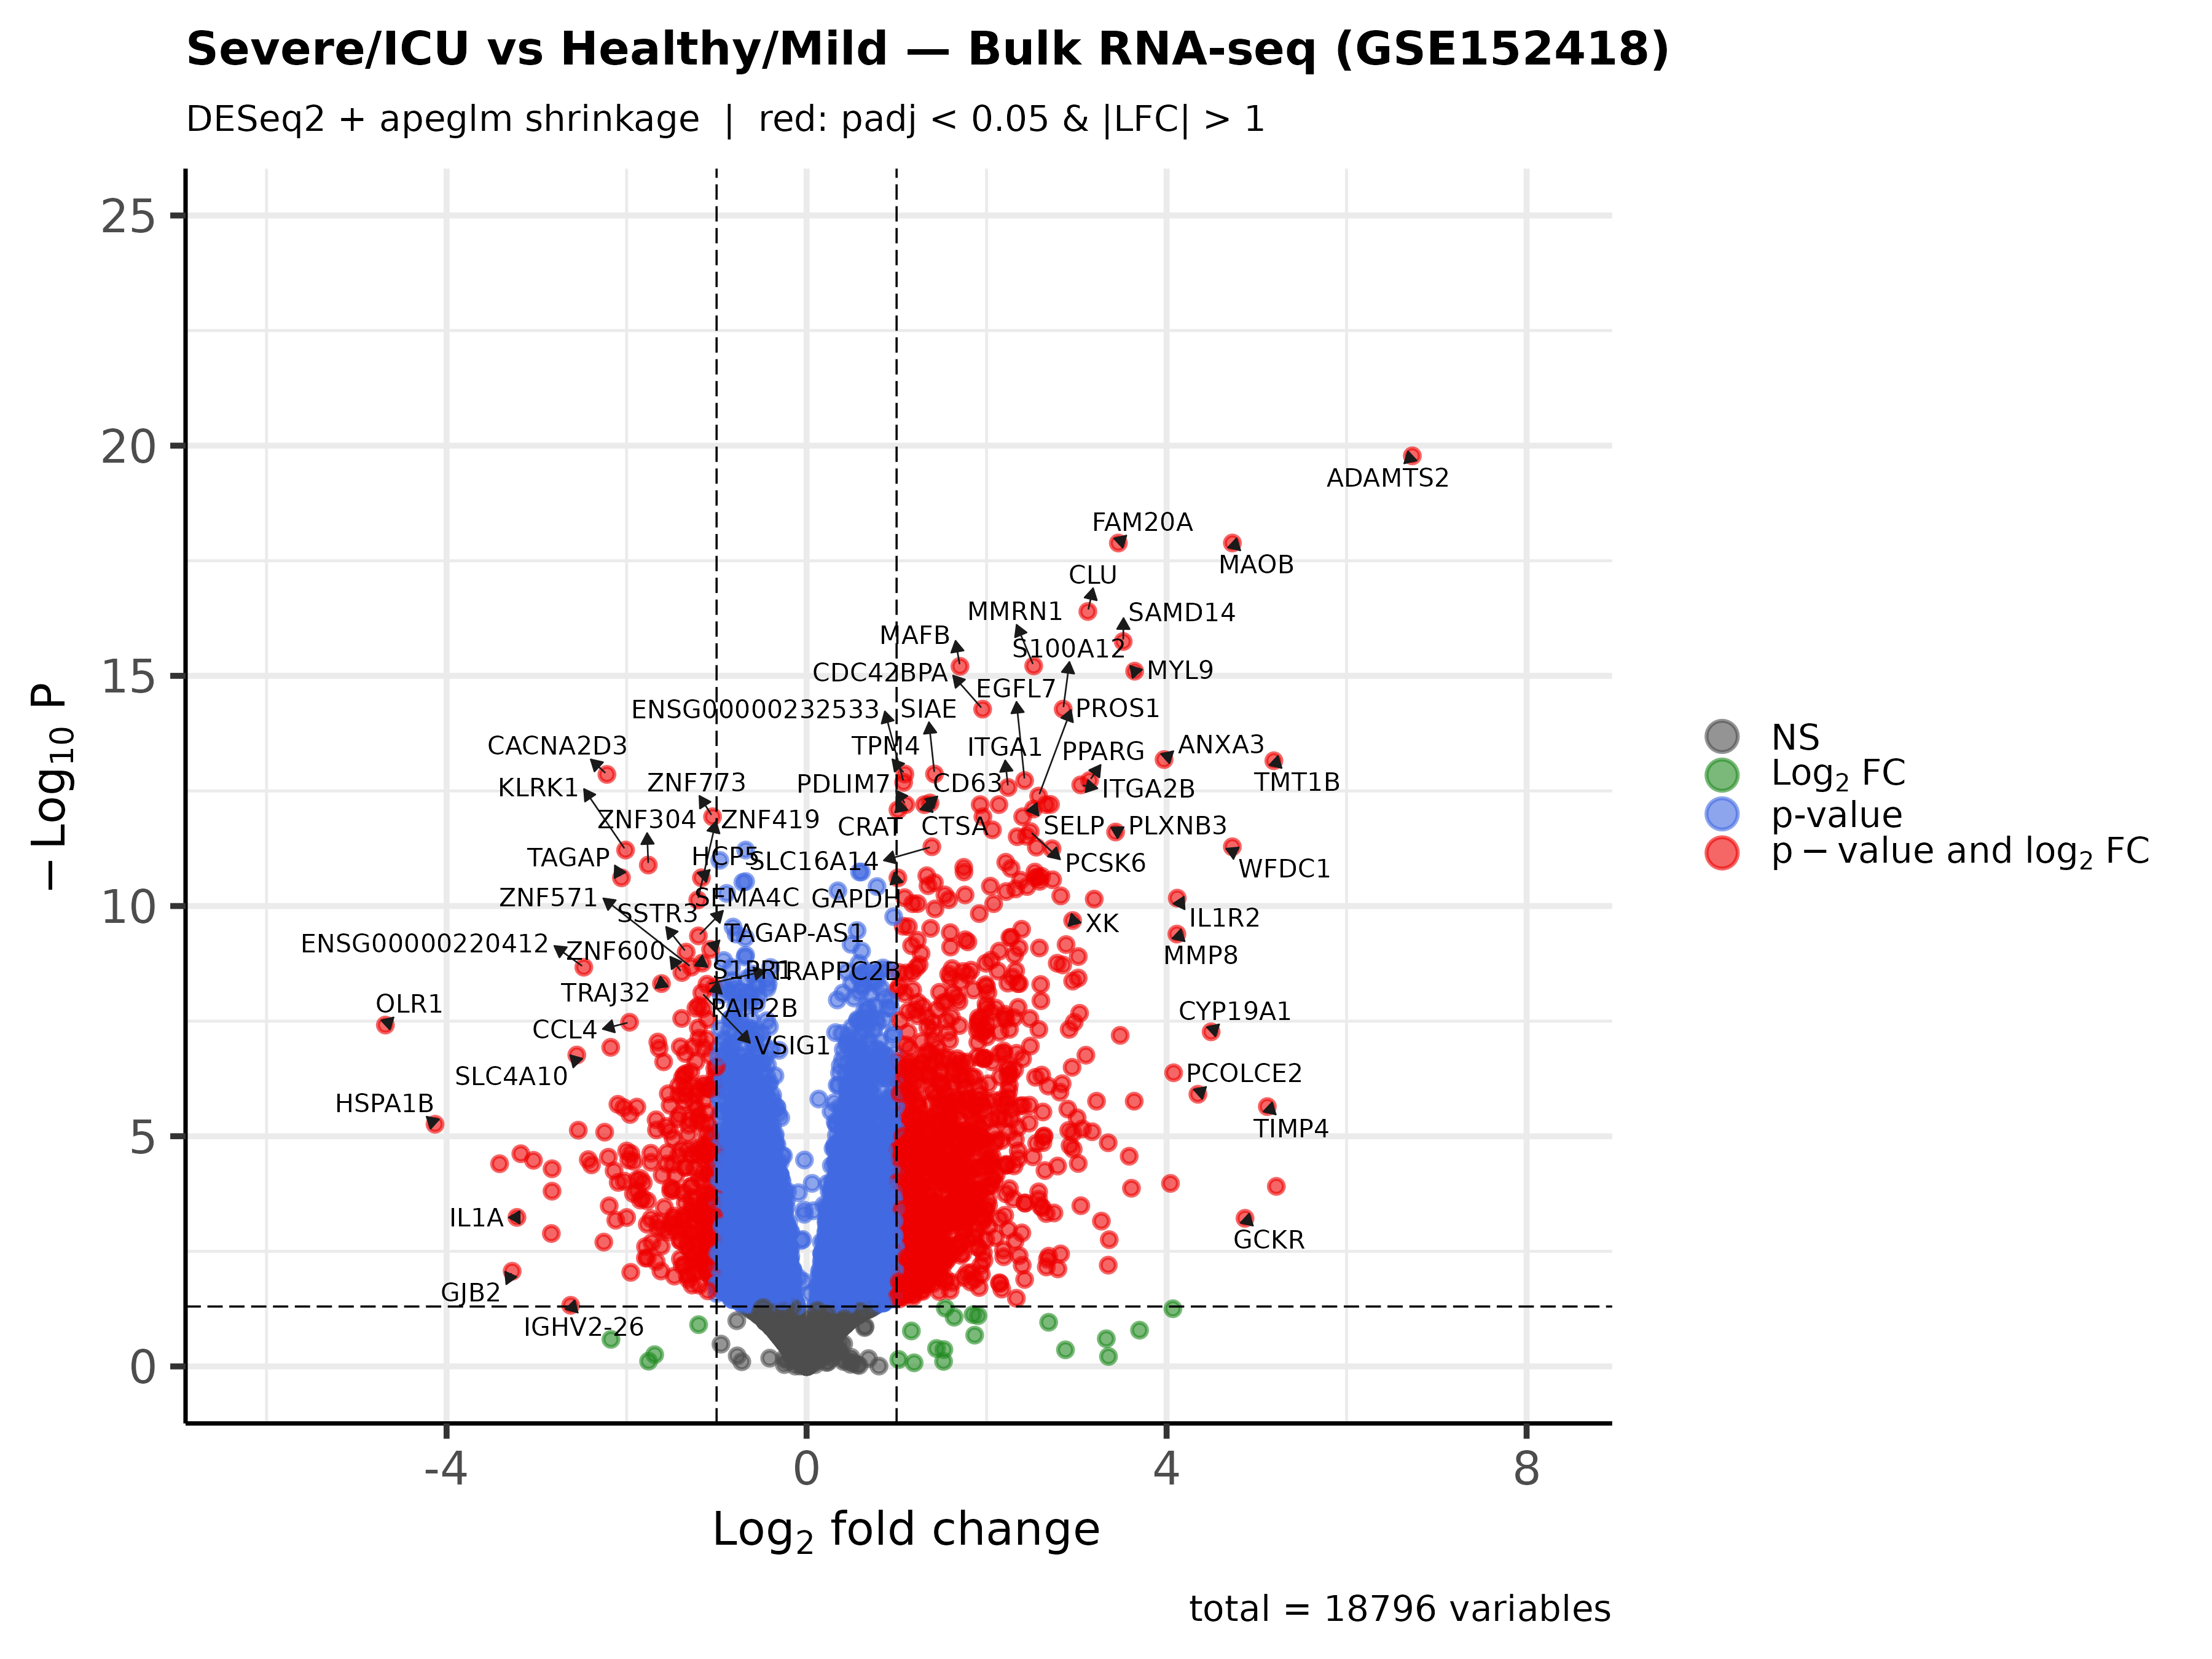
\includegraphics[width=\textwidth]{plots/phase10/phase10_volcano.png}
\end{center}

\textbf{$\sim$4,500 significant DE genes (padj $< 0.05$).}
The volcano reveals a pattern strikingly different from the scRNA-seq monocyte analysis:
\begin{itemize}[nosep]
  \item \textbf{Top upregulated}: ADAMTS2 (matrix remodeling, $\log_2$FC $\approx +8$),
        MMRN1 and ITGA2B (platelet structural proteins), S100A12 (emergency myeloid alarmin),
        MAFB and PPARG (monocyte-to-macrophage transcription factors).
        The signal is \textbf{myeloid and platelet expansion} — not the ISG or IL-1$\beta$
        programs from the scRNA-seq analysis.
  \item \textbf{Top downregulated}: OLR1 and KLRK1/NKG2D (NK cell receptors),
        TAGAP and CCL4 (T cell markers) — the \textbf{lymphocyte depletion} signal.
\end{itemize}

To directly test the project hypothesis, we inspected the key genes from the Phase 4
monocyte modules:

\begin{center}
  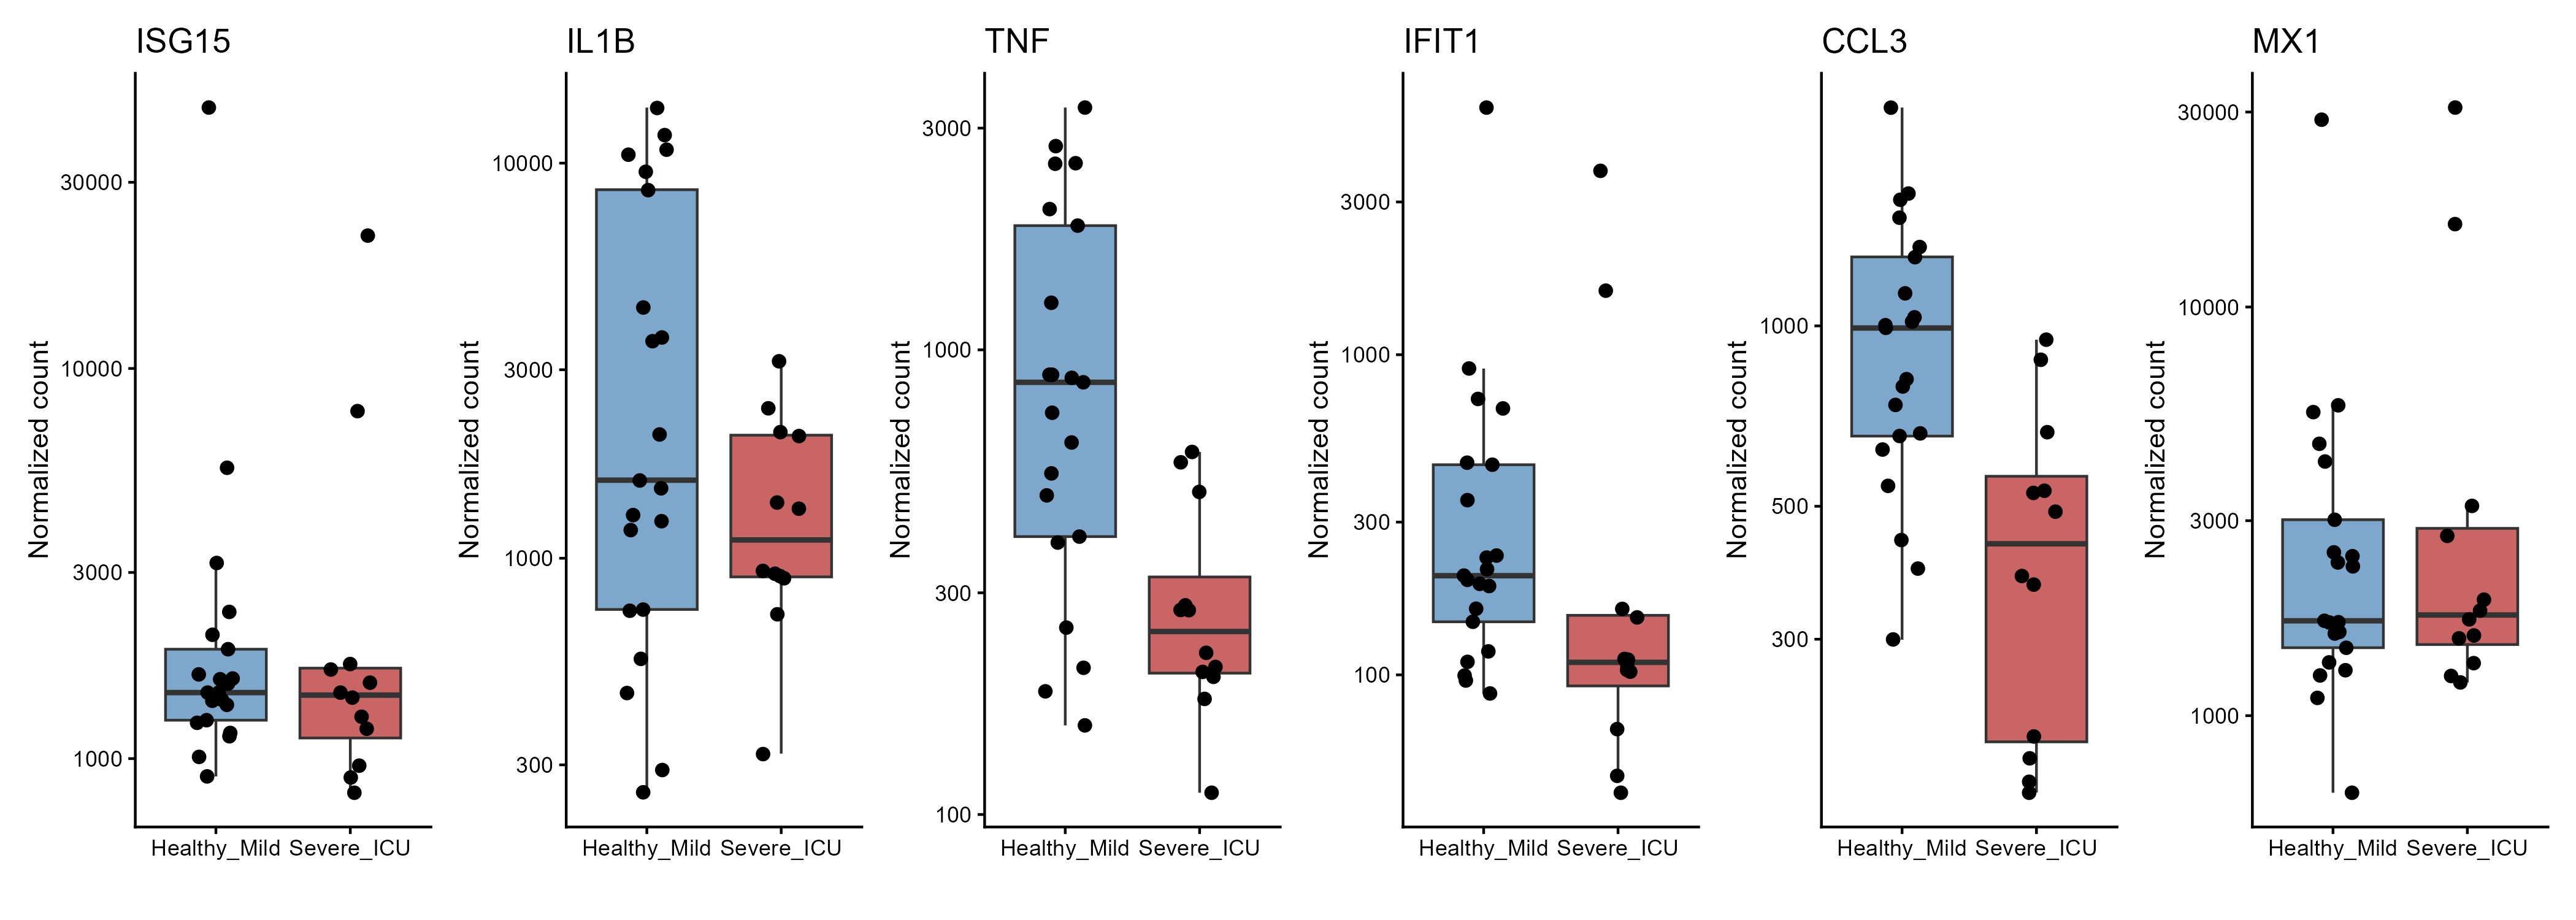
\includegraphics[width=\textwidth]{plots/phase8/phase8_key_gene_boxplots.png}
\end{center}

\textbf{None of the monocyte co-activation genes are upregulated in bulk blood.}
ISG15, IL1B, TNF, IFIT1, and CCL3 show no upward shift in Severe/ICU — several are
actually lower. The monocyte IL1B signal ($\log_2$FC $\approx +5$ in Phase 4) has
completely vanished.

The explanation is the dilution effect: T cells and NK cells, which are depleted in
severe COVID, are baseline producers of TNF, CCL3, and ISGs. Their loss removes more
signal than the minority monocyte sub-clusters can add back. The bulk net change is
near zero or negative for all these genes.

% ═══════════════════════════════════════════════
\section{Phase 9 — Adjusting for the Gender Confounder}
% ═══════════════════════════════════════════════

The extended DESeq2 model \texttt{\textasciitilde gender + severity\_group} was fit
to correct for the gender imbalance identified in Phase 7.
If the Phase 8 results were driven by sex-biased genes rather than COVID severity,
they would collapse under this correction.

\begin{center}
  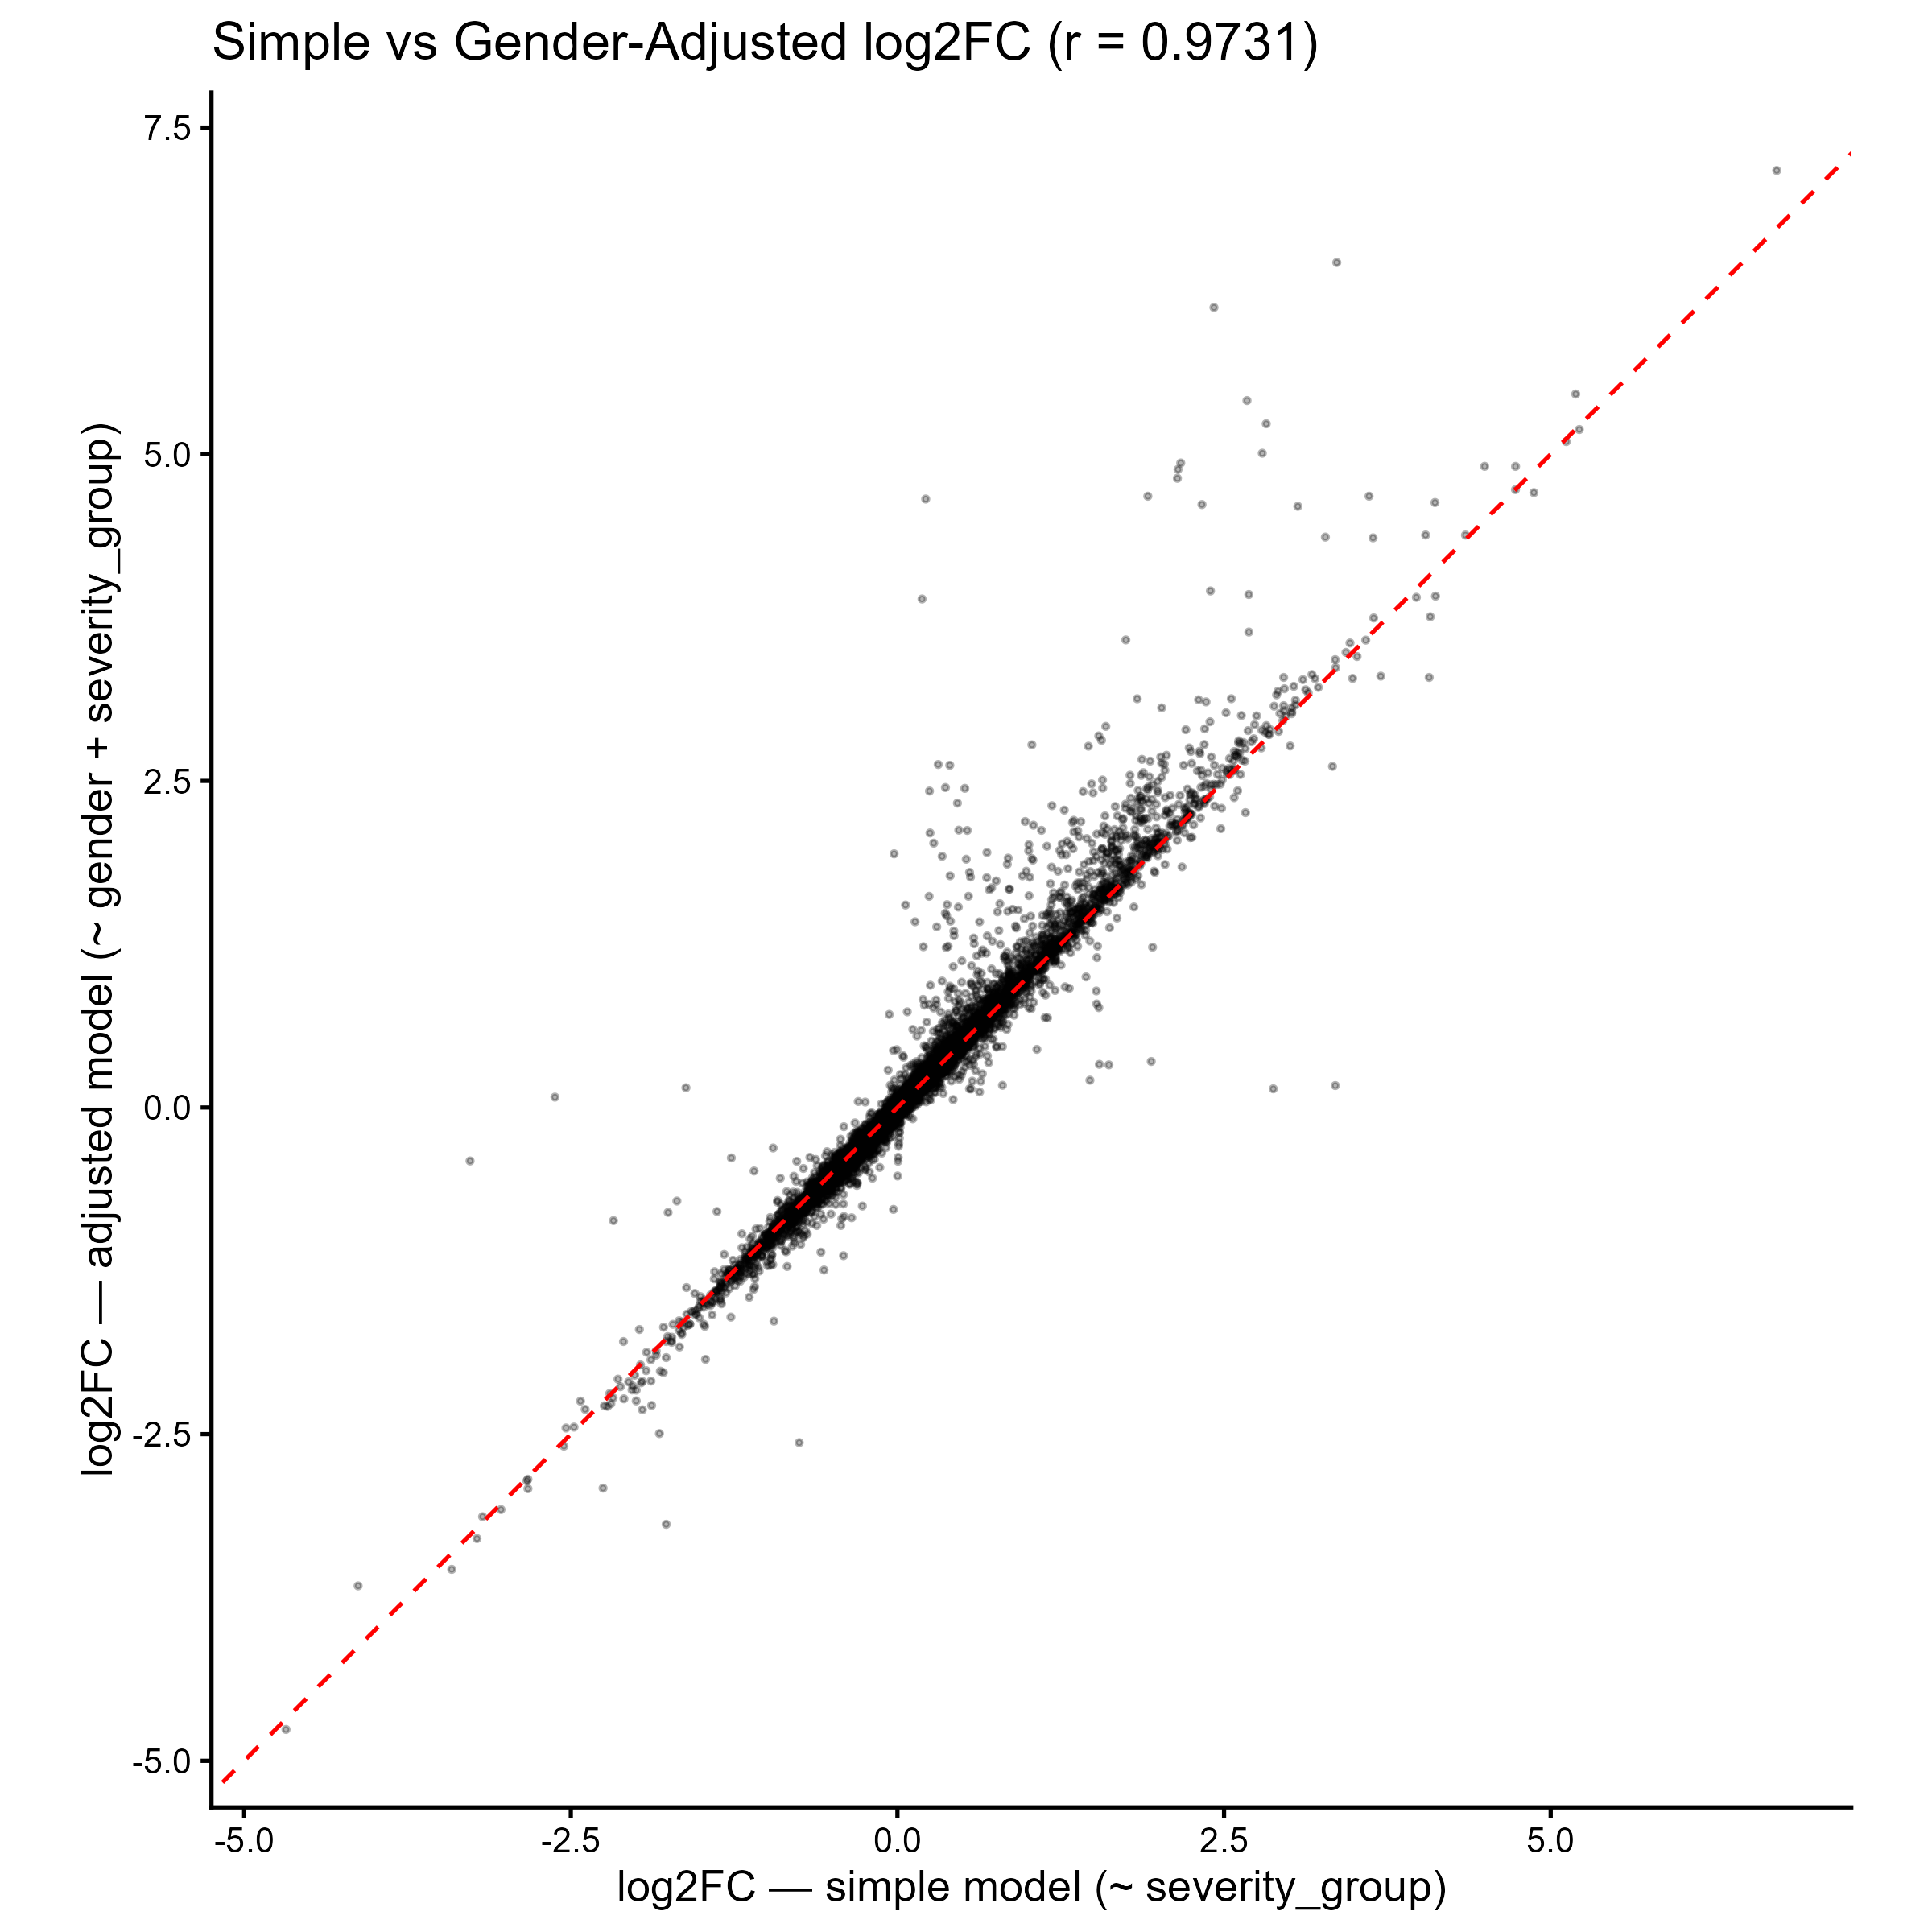
\includegraphics[width=0.82\textwidth]{plots/phase9/phase9_lfc_correlation.png}
\end{center}

The fold-changes from the simple and gender-adjusted models correlate at
\textbf{Pearson $r = 0.97$}. The cloud hugs the diagonal — every gene that was
significant remains significant, and directions are unchanged.
Gender explains only $\sim$3\% of fold-change variance. The Phase 8 results are robust,
and the gender-adjusted model is used in all subsequent phases.

% ═══════════════════════════════════════════════
\section{Phase 10 — Bulk Visualization: The Co-Activation Paradox}
% ═══════════════════════════════════════════════

With a validated DE gene list, we directly test whether the ISG and TNF/IL-1$\beta$
programs are elevated in bulk blood — using the same 6-gene panels that defined the
Phase 4 modules.

\begin{center}
  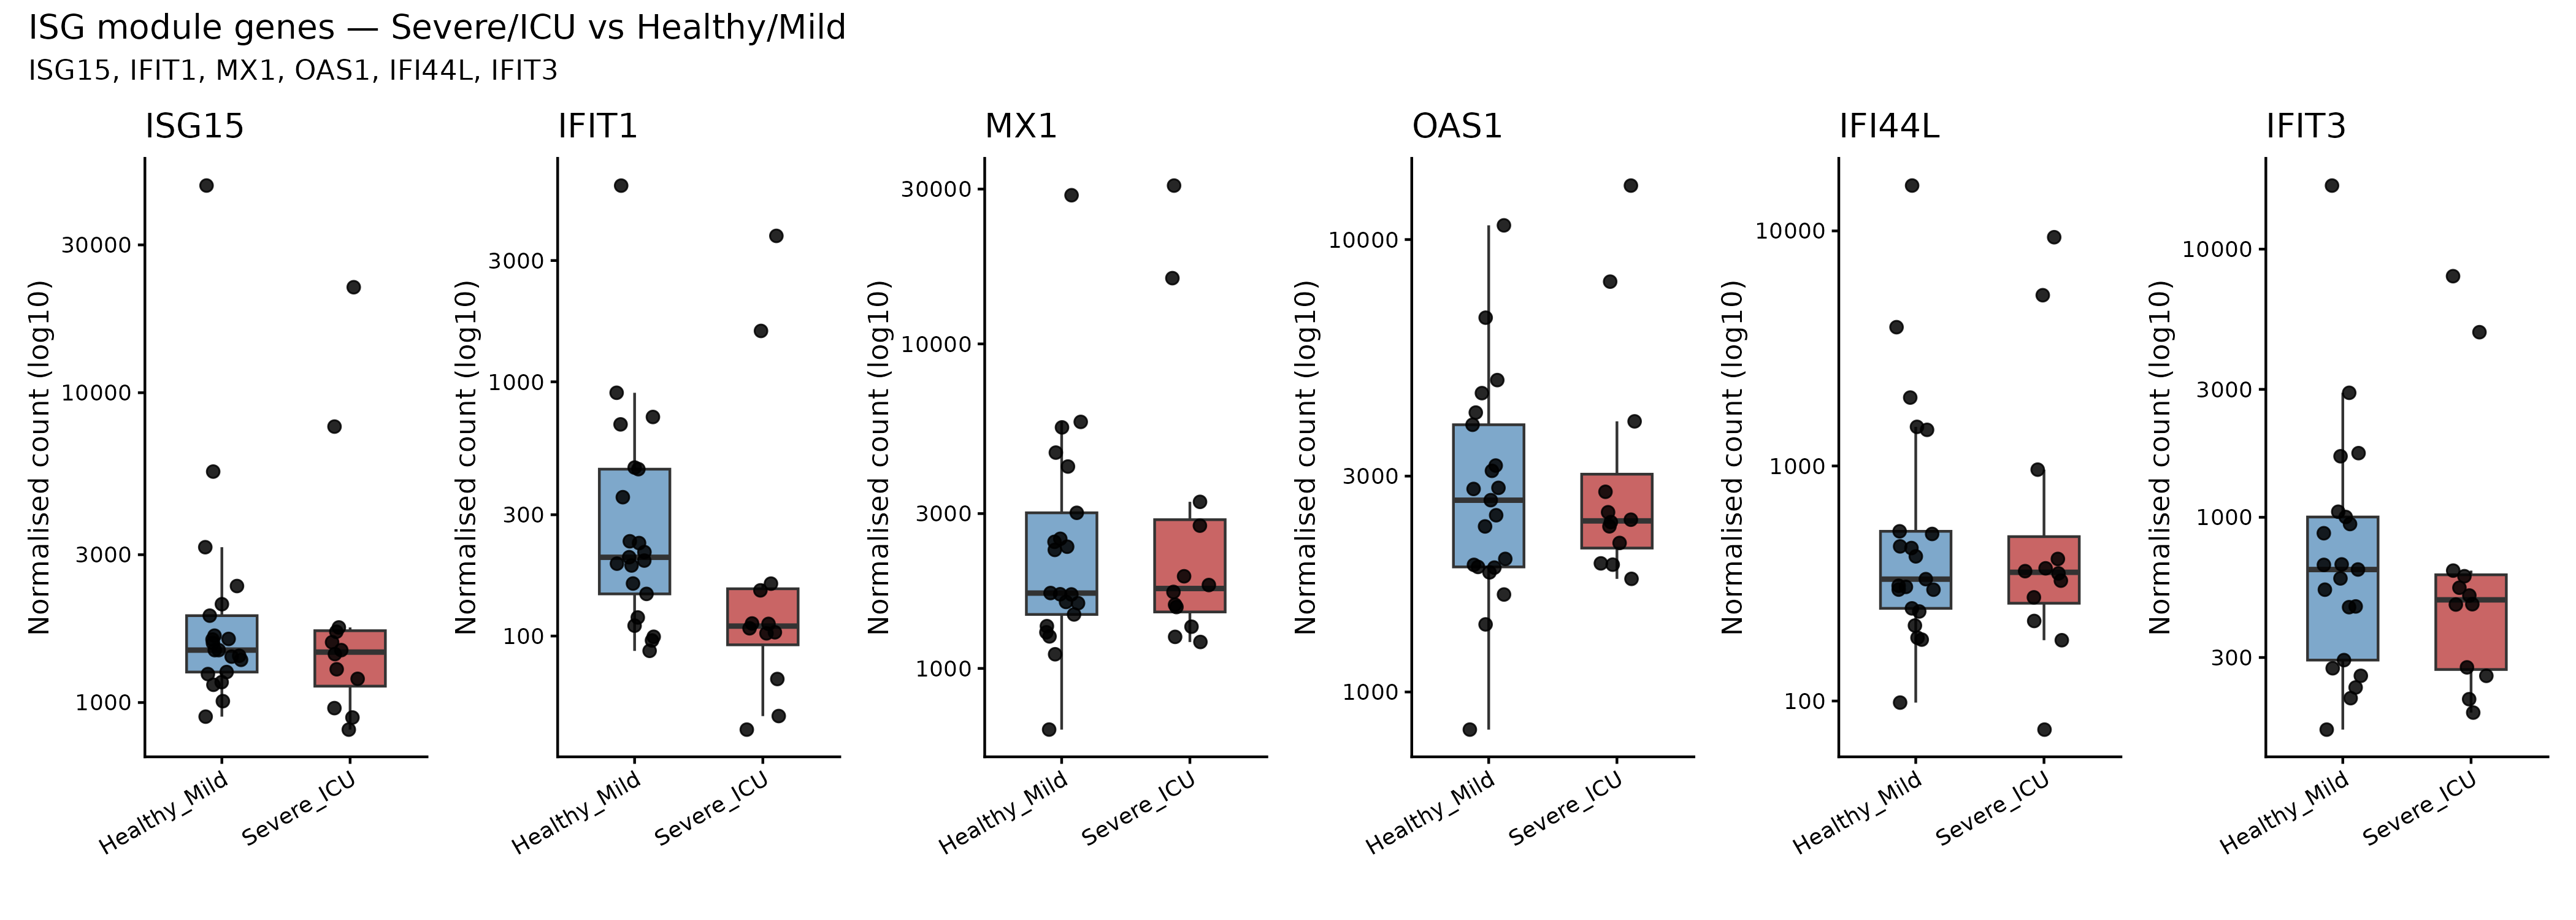
\includegraphics[width=\textwidth]{plots/phase10/phase10_ISG_panel.png}
\end{center}

Across all six ISG genes (ISG15, IFIT1, MX1, OAS1, IFI44L, IFIT3), there is no
consistent elevation in Severe/ICU. Boxes overlap or are slightly lower in Severe.

\begin{center}
  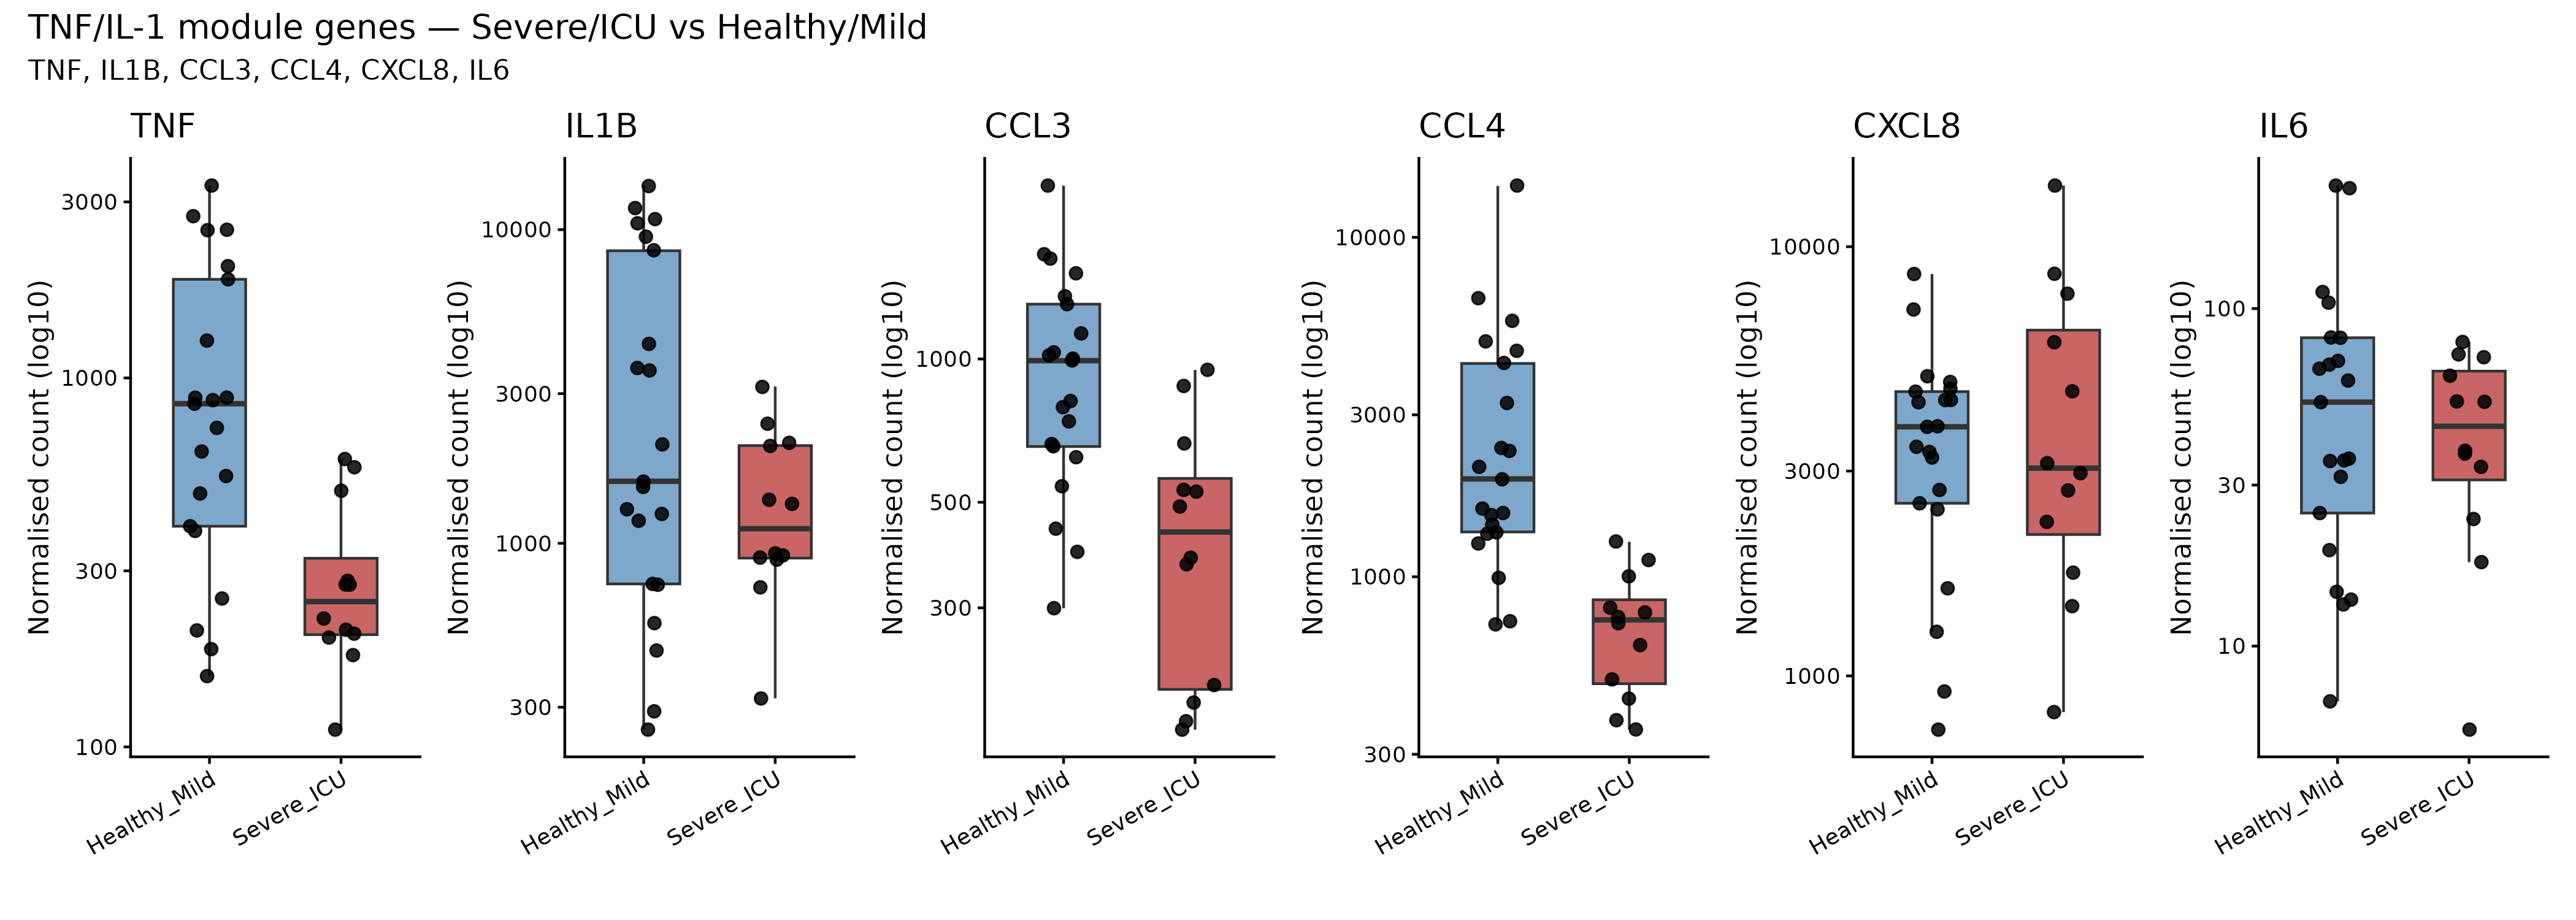
\includegraphics[width=\textwidth]{plots/phase10/phase10_TNF_IL1_panel.png}
\end{center}

Every TNF/IL-1$\beta$ gene (TNF, IL1B, CCL3, CCL4, CXCL8, IL6) is \textit{lower}
or unchanged in Severe/ICU whole blood — with TNF, IL1B, CCL3, and CCL4 clearly
below the Healthy/Mild median.
This is the direct, per-gene demonstration of the dilution paradox:
the monocyte-level finding from Phase 4 is invisible from the blood-level view of Phase 8.

% ═══════════════════════════════════════════════
\section{Phase 11 — PCA and Unsupervised Clustering}
% ═══════════════════════════════════════════════

Individual gene tests show which genes change, but do the samples as a whole
self-organise by severity without any label input?
This is the strongest validation that the transcriptomic difference is real and pervasive —
not a few noisy genes but a global signal.

VST-normalized expression of the 1,000 most variable genes was used for PCA,
hierarchical clustering, and k-means, all blind to severity labels.

\begin{center}
  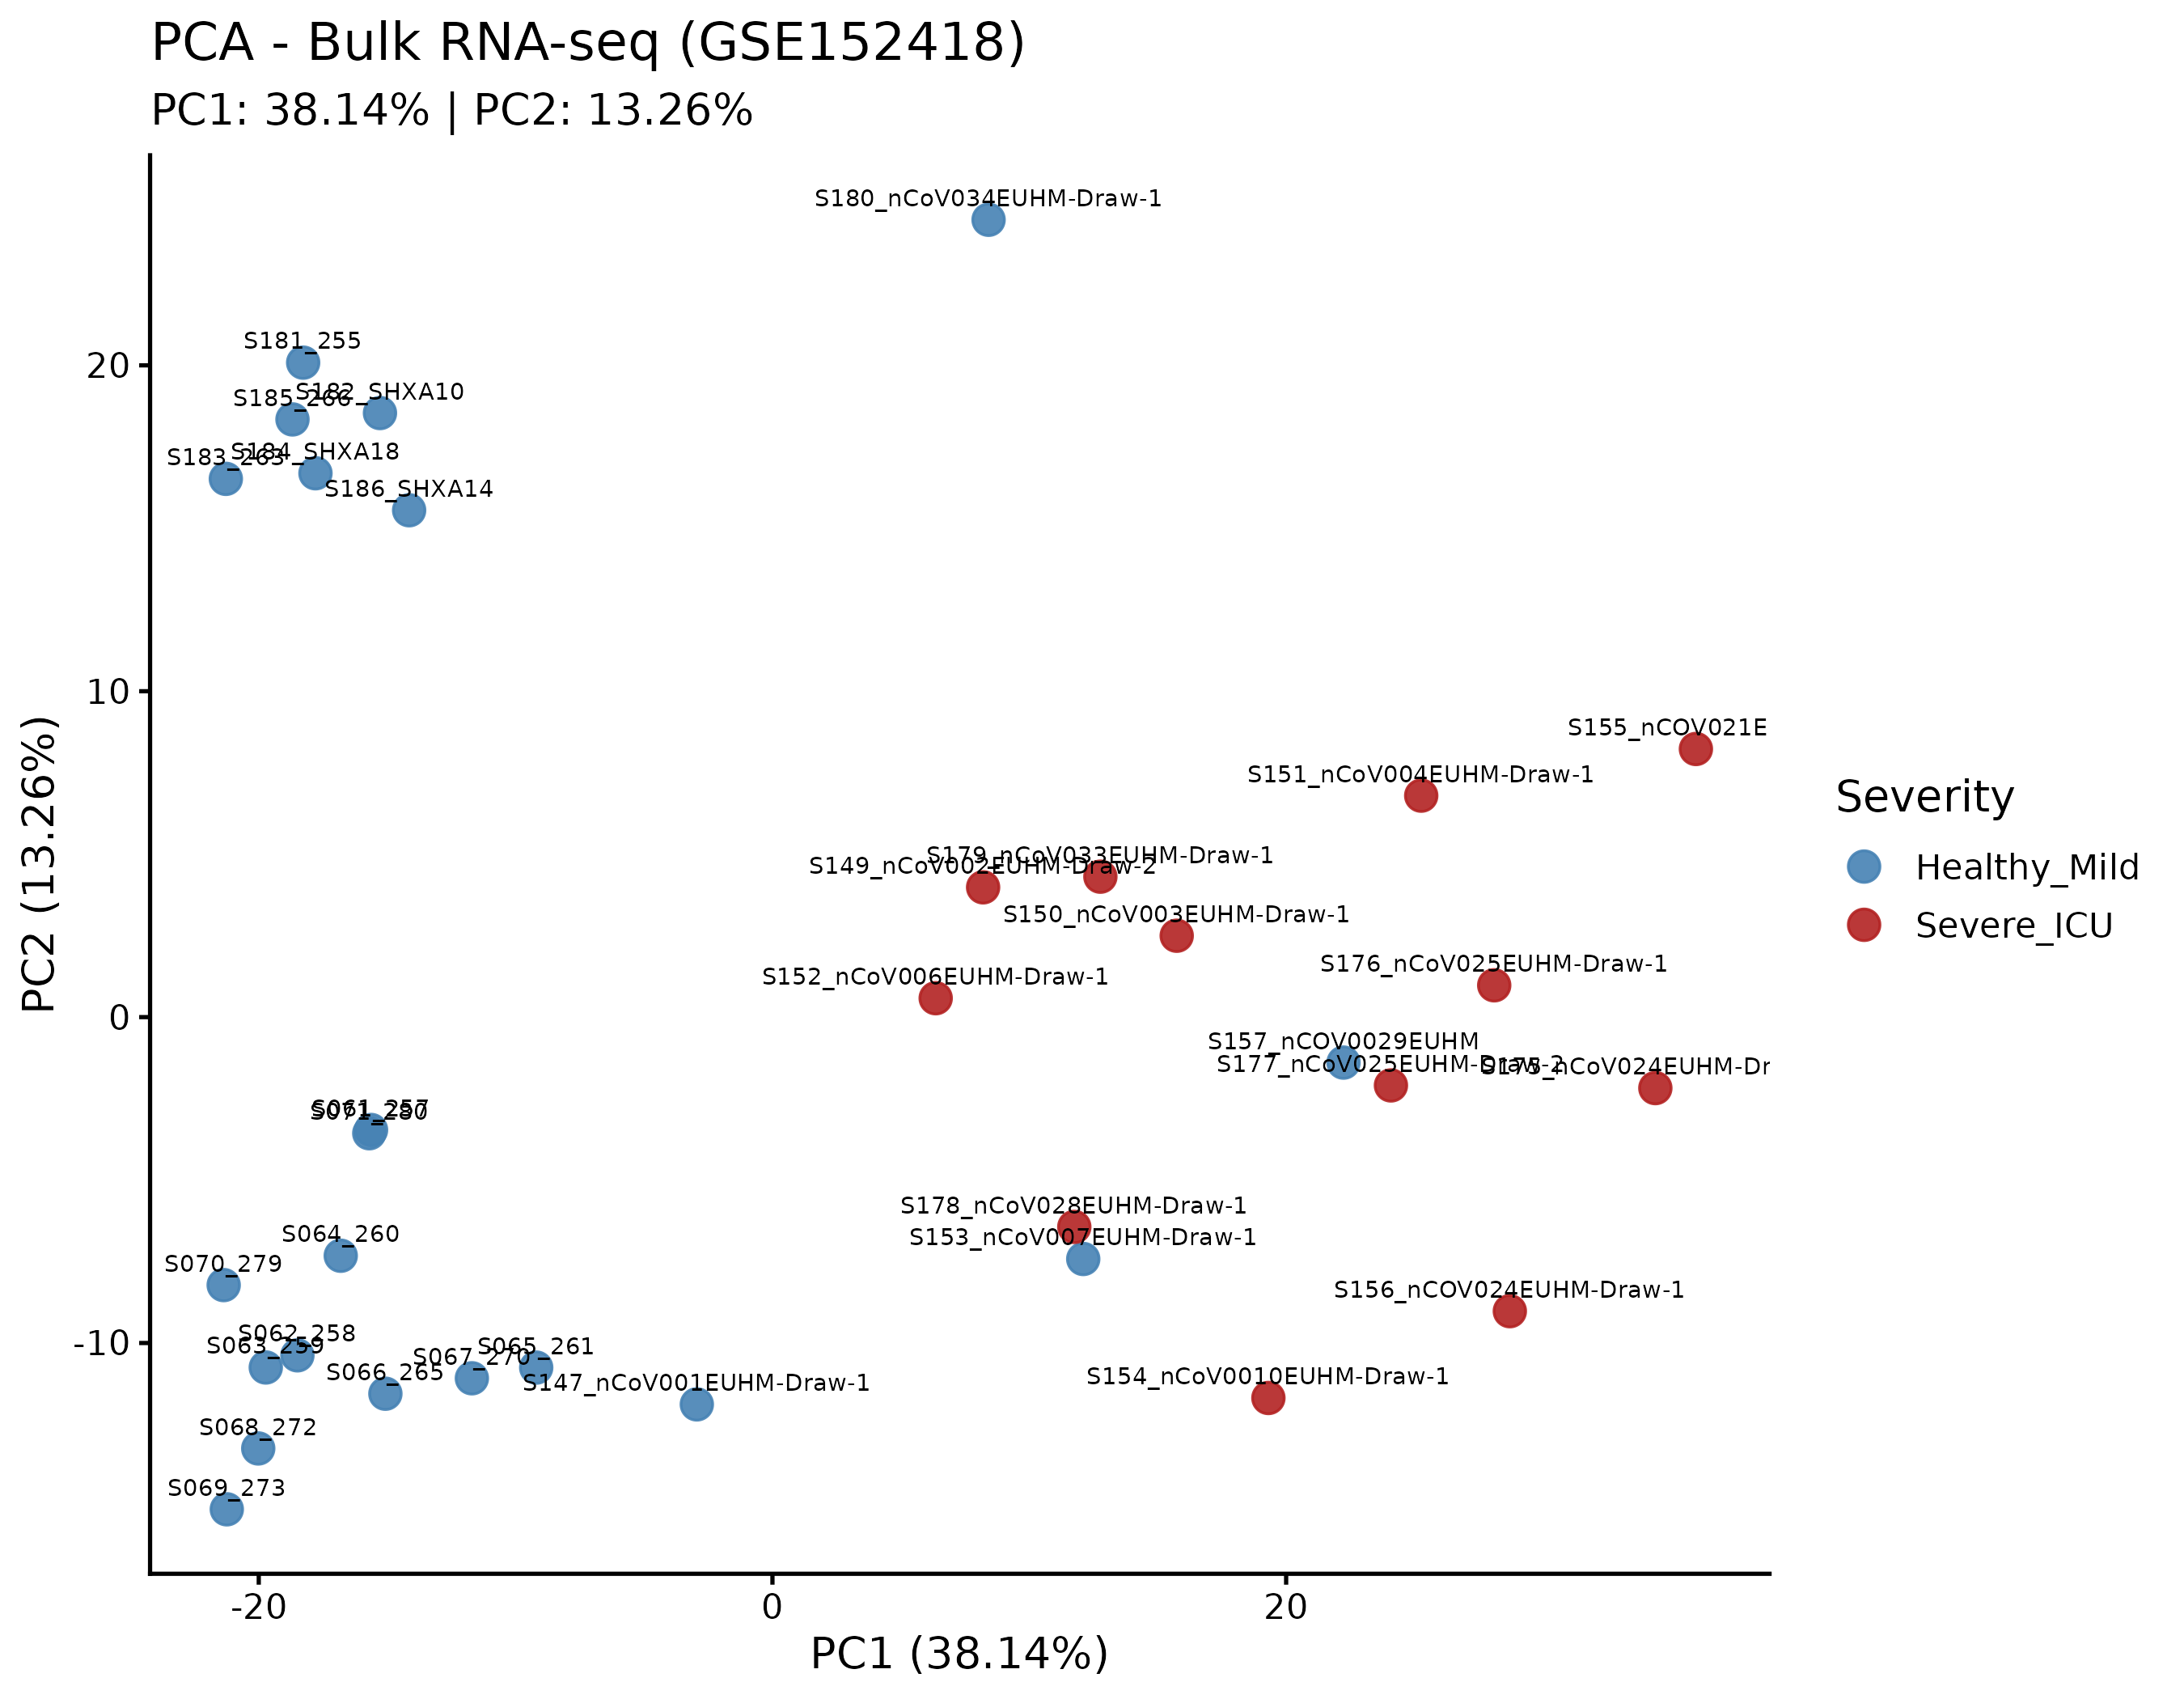
\includegraphics[width=0.88\textwidth]{plots/phase11/phase11_PCA_severity.png}
\end{center}

\textbf{PC1 (38\% of variance) perfectly separates the two groups.}
Every Healthy/Mild sample sits at negative PC1; every Severe/ICU sample at positive PC1.
Zero overlap. PC2 shows no severity structure — it captures within-condition donor variability.
A single axis of gene expression encodes whether a patient is critically ill.

\begin{center}
  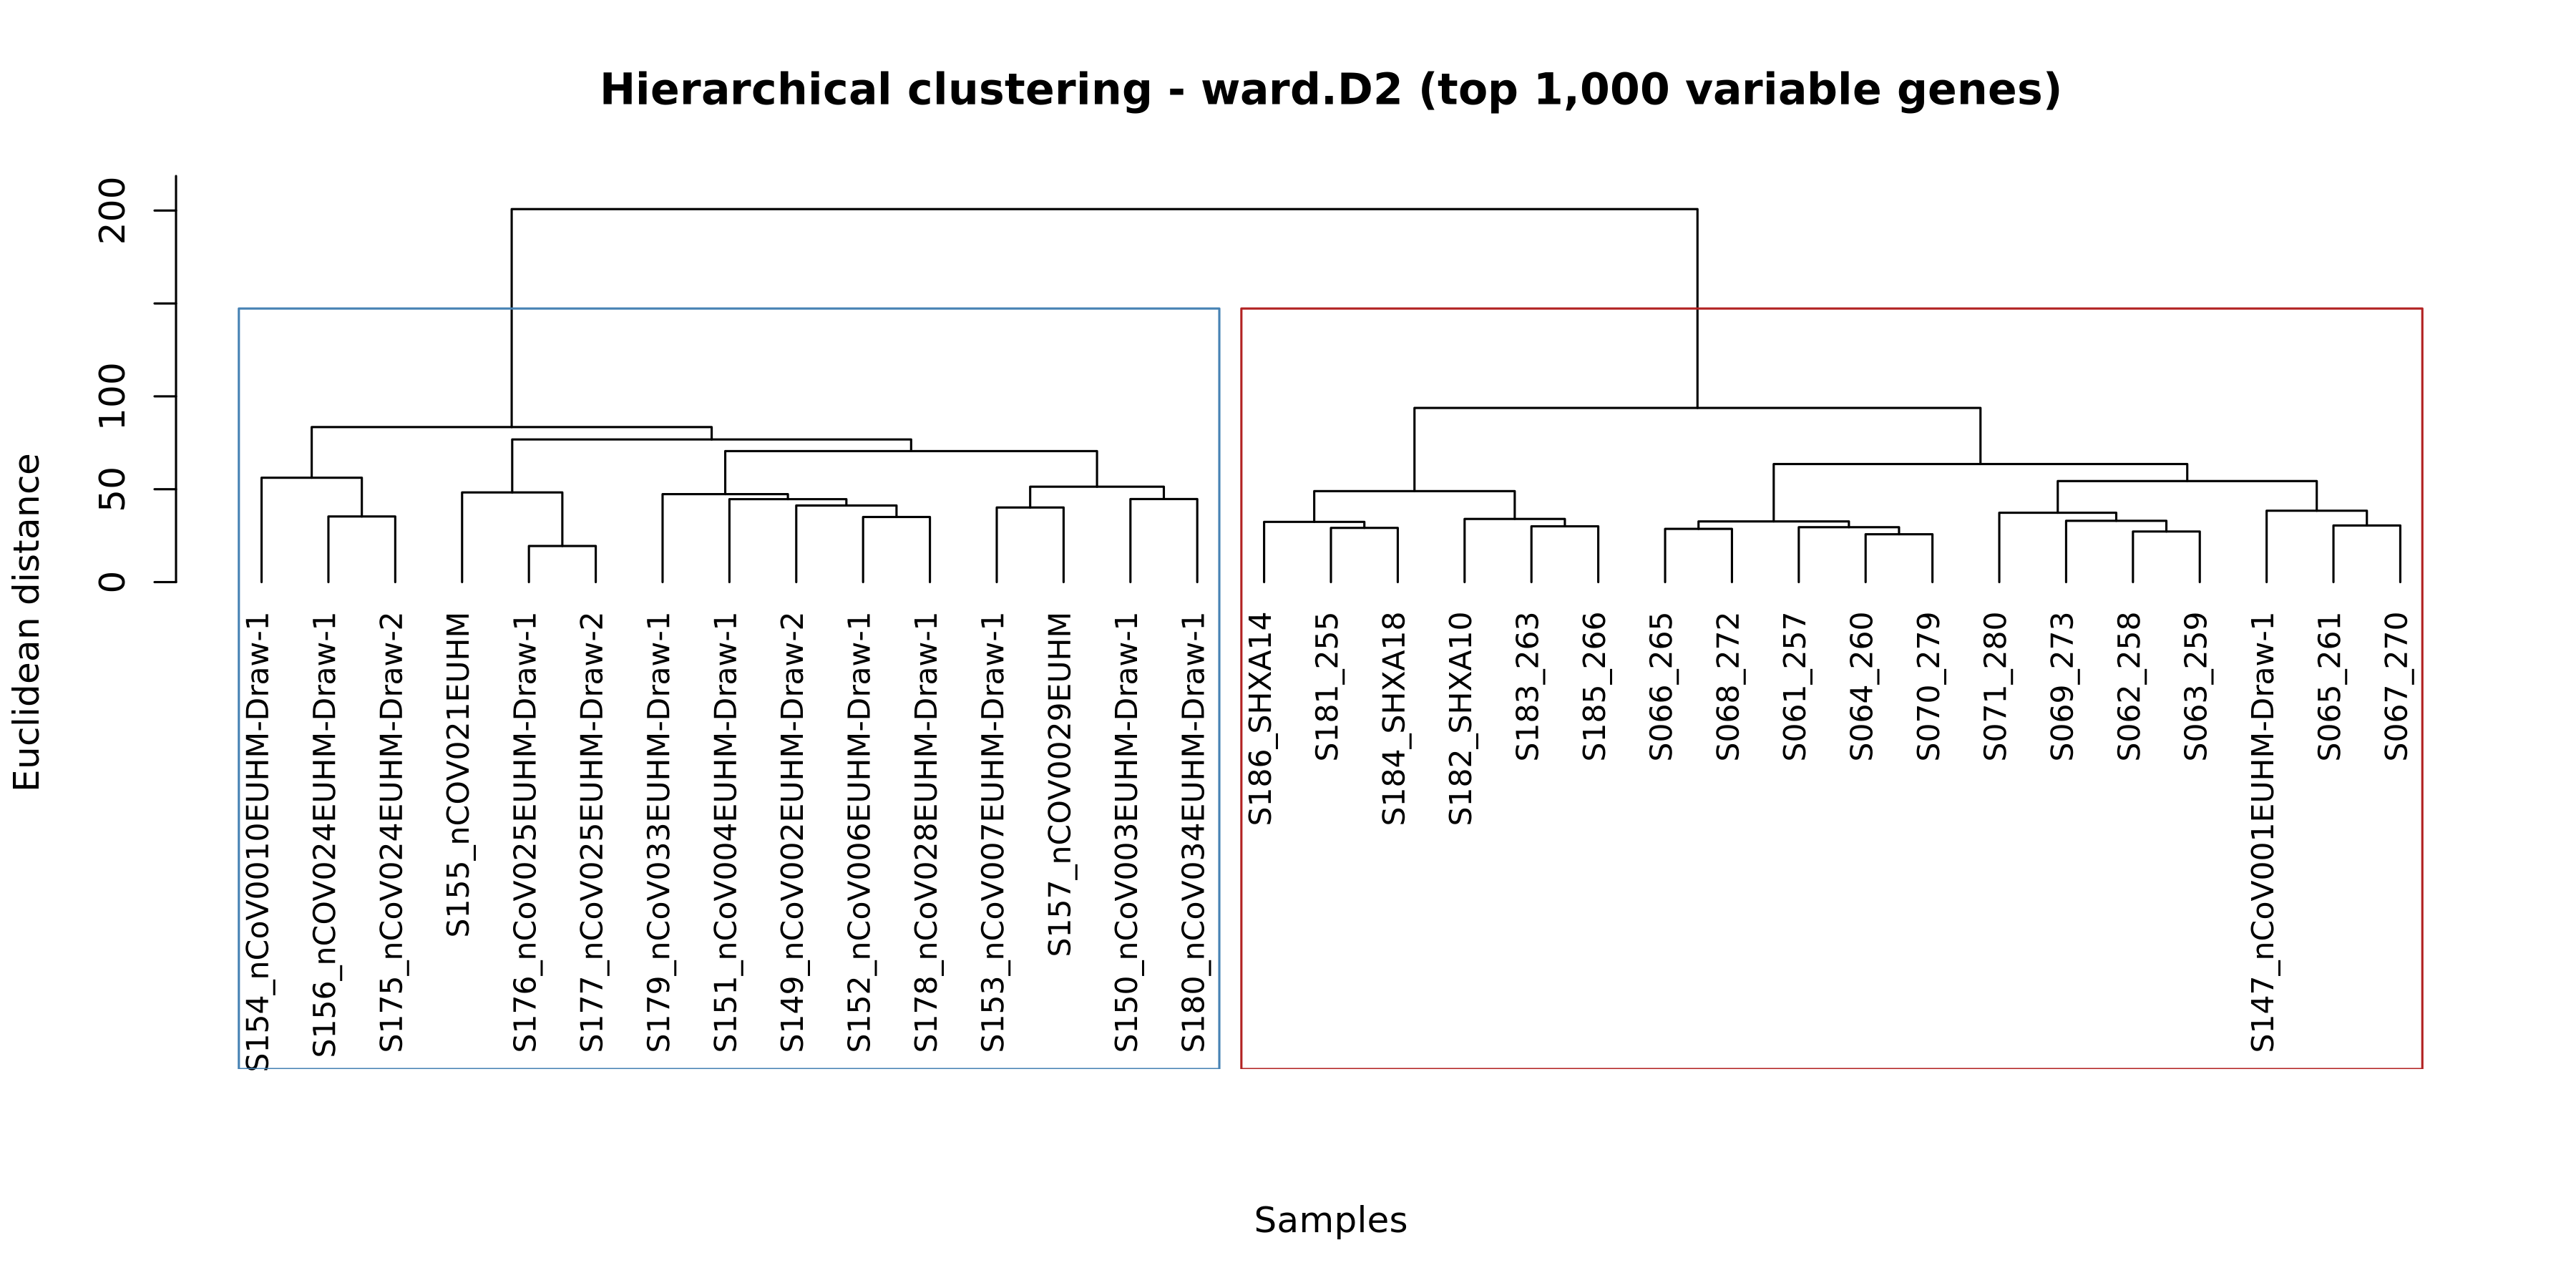
\includegraphics[width=\textwidth]{plots/phase11/phase11_hierarchical_clustering.png}
\end{center}

Hierarchical clustering (Ward.D2) and k-means ($k=2$) independently recover the two
severity groups with \textbf{97\% accuracy (32/33 correct)}, flagging the same single
Severe outlier whose transcriptome resembles Healthy — likely a patient at an atypical
disease stage.

The bulk transcriptome of severe COVID blood is categorically different from Healthy at
the whole-expression level, not just at individual genes.

% ═══════════════════════════════════════════════
\section{Phase 12 — GSEA Pathway Analysis}
% ═══════════════════════════════════════════════

PCA and clustering confirmed the separation. GSEA now answers: \textit{what biological
programs drive it?}
Rather than asking which individual genes change, Gene Set Enrichment Analysis tests
whether coordinated programs shift as a whole — detecting signals that no single gene
would reveal alone.
Four databases were used (GO:BP, Hallmark, KEGG, Reactome) as independent cross-validation.

\begin{center}
  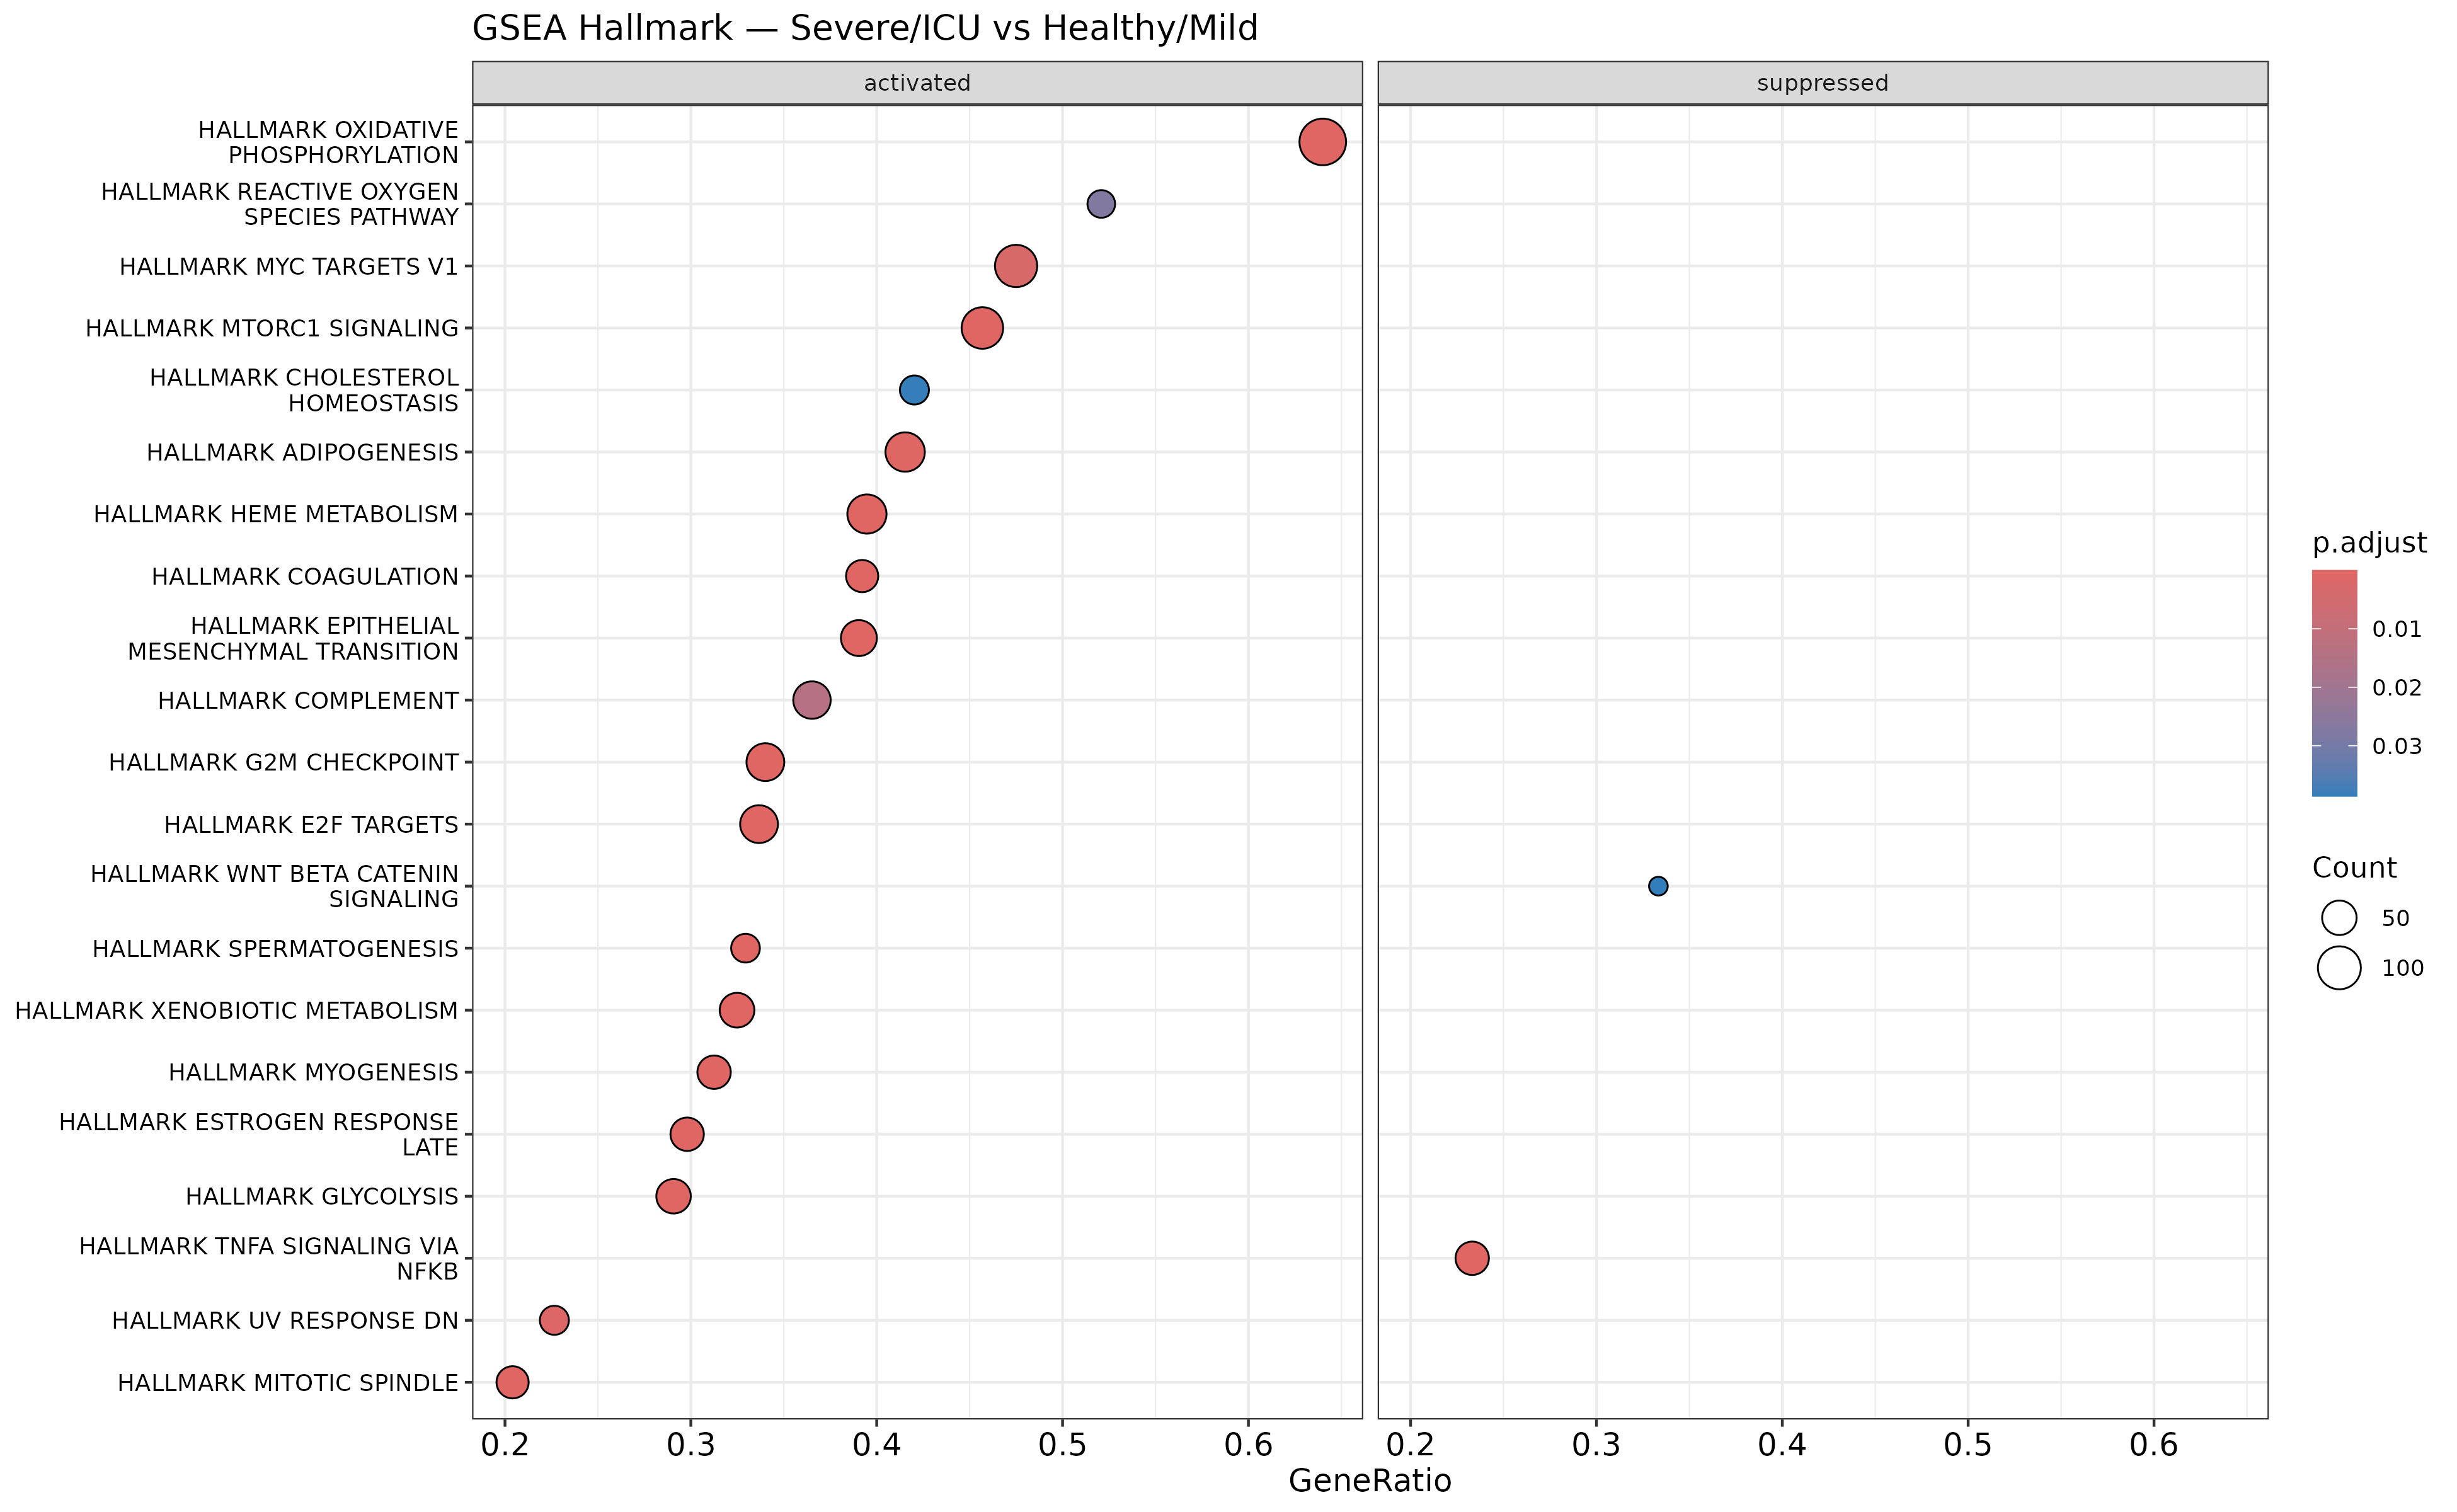
\includegraphics[width=0.92\textwidth]{plots/phase12/phase12_hallmark_dotplot.png}
\end{center}

The Hallmark dotplot tells the bulk story in one figure:
\begin{itemize}[nosep]
  \item \textbf{Activated in Severe}: Oxidative Phosphorylation (top program, GeneRatio
        $\approx 0.65$), Reactive Oxygen Species, MYC Targets, mTORC1, Coagulation,
        Complement, G2M Checkpoint. This is a picture of cells actively proliferating,
        running on mitochondrial metabolism, and driving innate coagulation — the emergency
        myeloid/platelet expansion from Phase 8, expressed as gene programs.
  \item \textbf{Suppressed in Severe}: \textbf{TNF$\alpha$ Signaling via NF-$\kappa$B}.
        This is the most important result of the bulk analysis. The very inflammatory
        program that was strongly upregulated in individual monocytes (Phase 4) is a
        \textit{net loss} in whole blood.
\end{itemize}

\begin{center}
  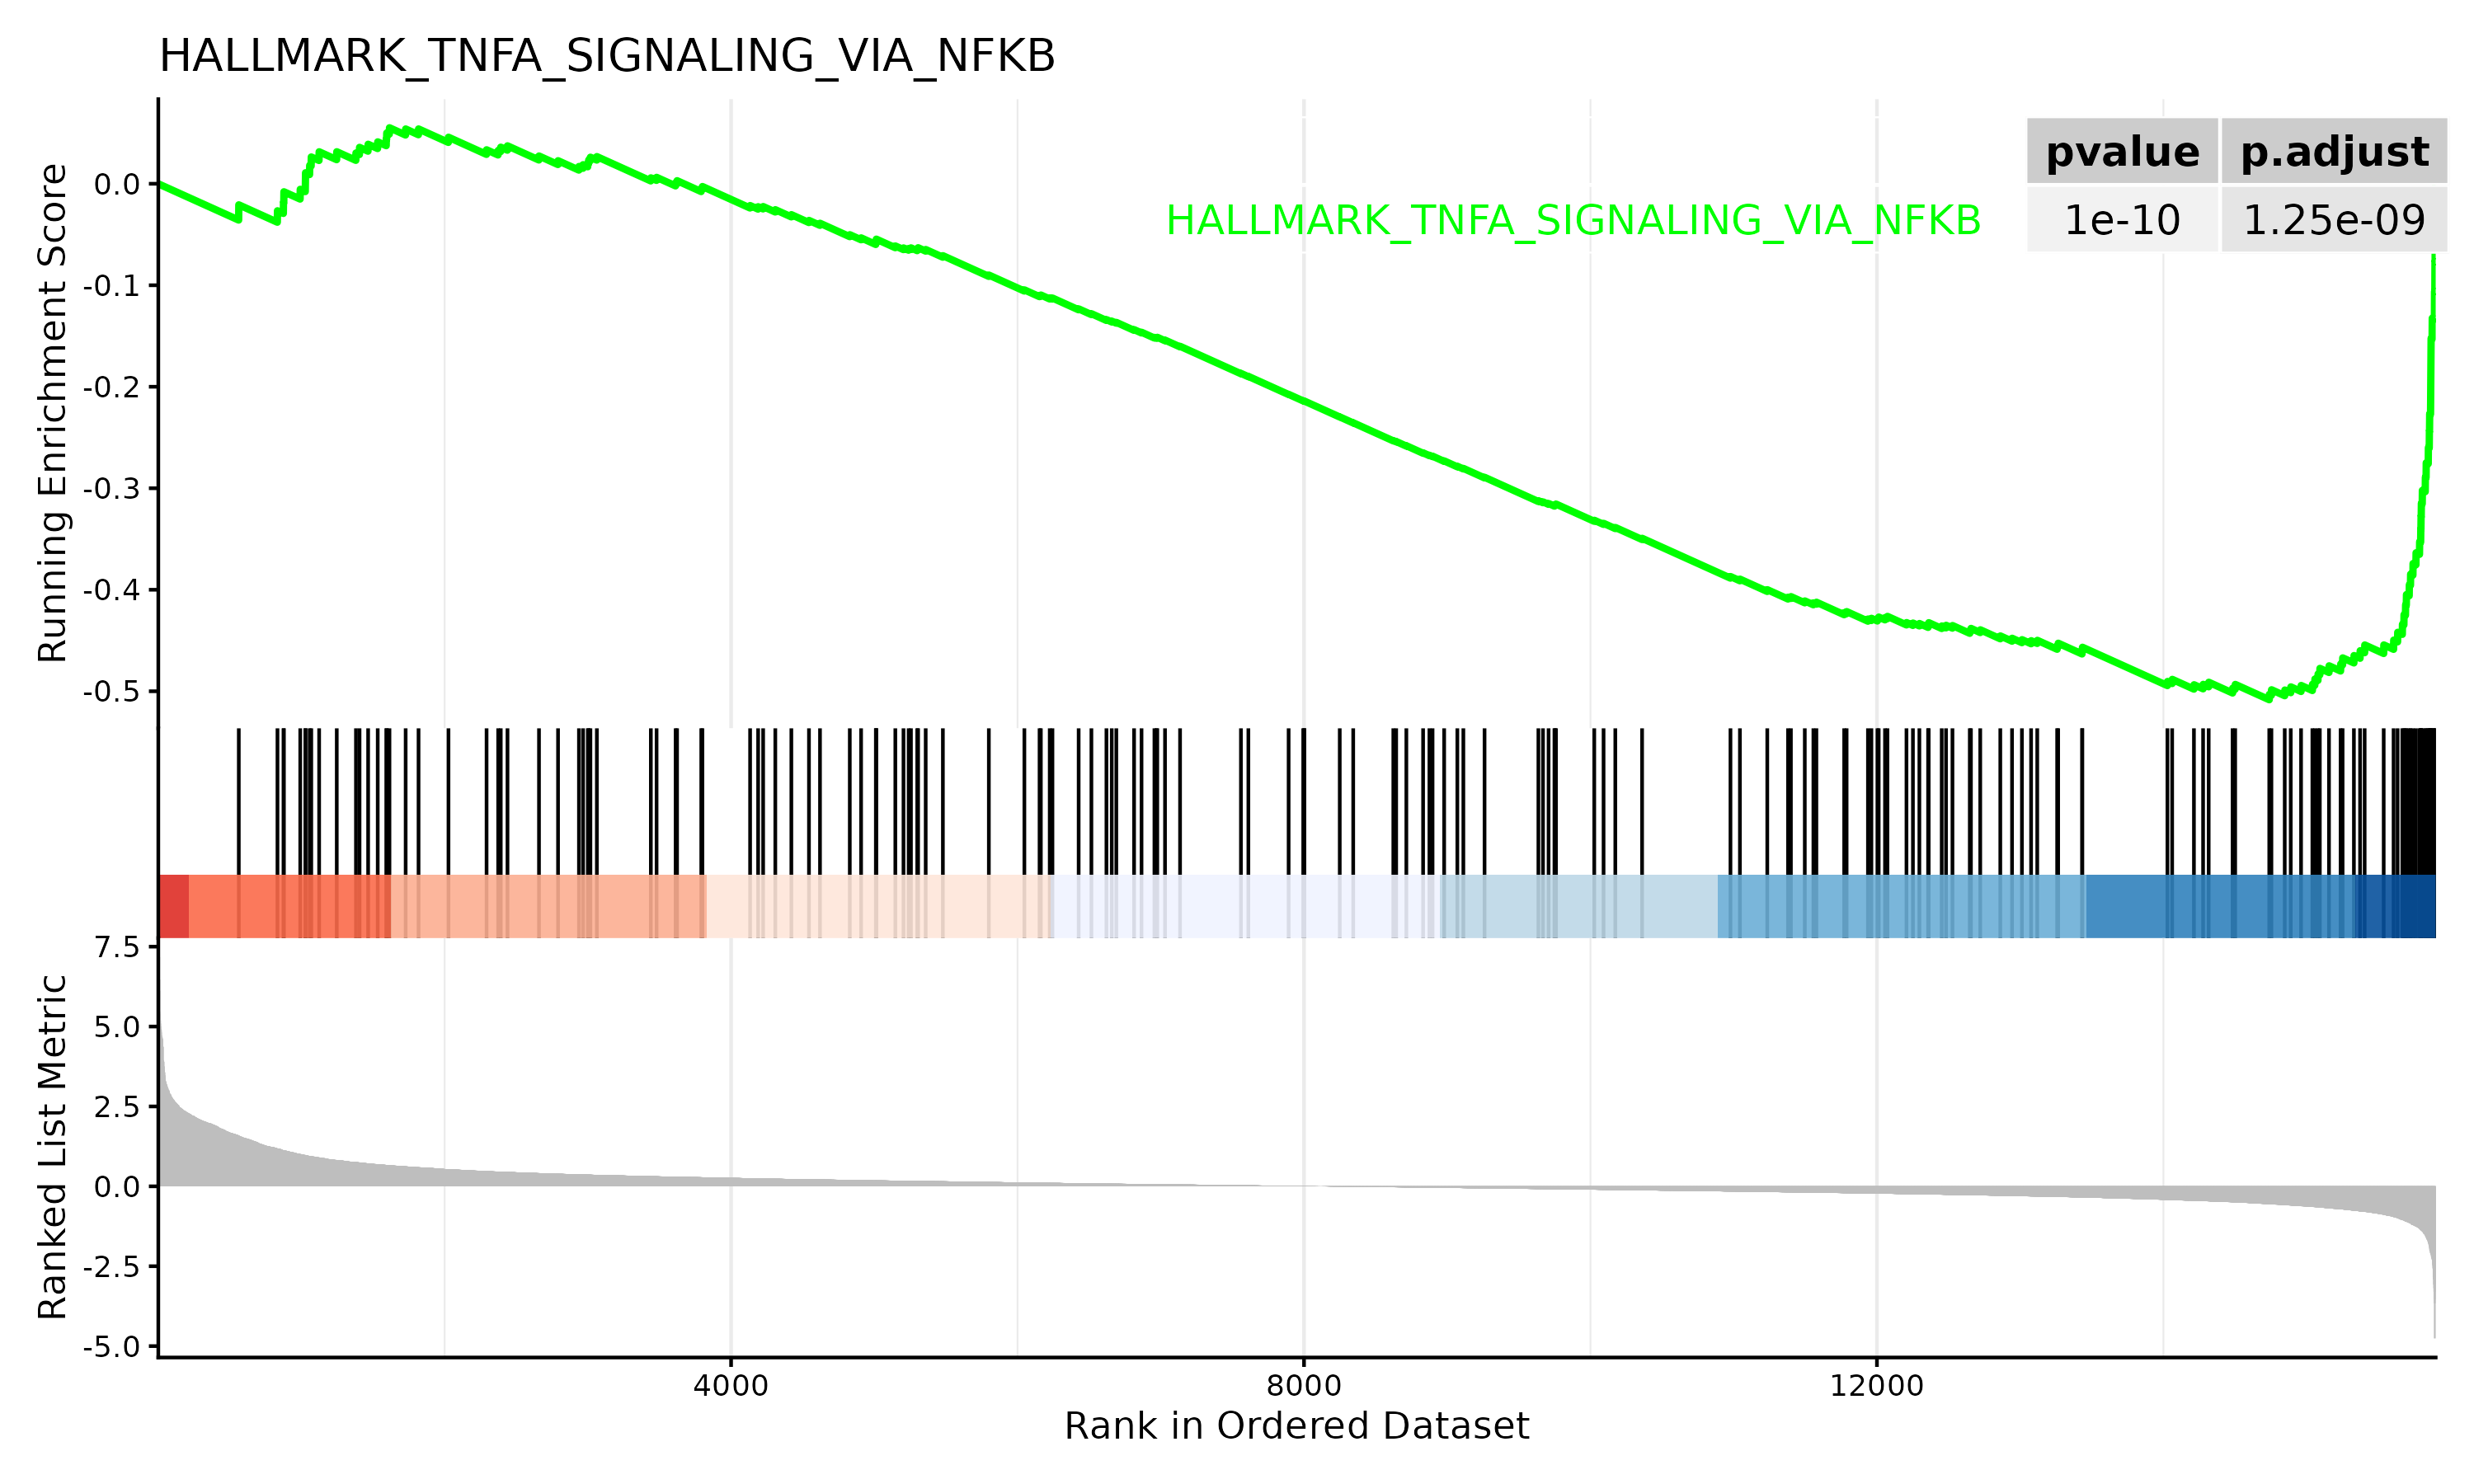
\includegraphics[width=0.88\textwidth]{plots/phase12/phase12_gsea_TNF_NFKB.png}
\end{center}

The TNF/NF-$\kappa$B enrichment plot confirms this unambiguously: the green running-sum
curve dips immediately below zero and continues falling. The TNF/NF-$\kappa$B gene set
is concentrated at the \textit{downregulated} end of the ranked list
($p = 10^{-10}$, padj $= 1.25 \times 10^{-9}$).
This is the pathway-level confirmation that the inflammatory signal visible in monocytes
(Phase 4) is overwhelmed by lymphocyte loss at the bulk level.

Reactome additionally identified \textbf{circadian clock disruption} (BMAL1/CLOCK targets
as the most suppressed Reactome pathway) — a novel finding suggesting that the circadian
immune regulation machinery is dismantled in ICU patients, which may independently
worsen outcomes.

% ═══════════════════════════════════════════════
\section{Phase 13 — Monocyte Co-Activation Signature in Bulk}
% ═══════════════════════════════════════════════

Three bulk methods have now shown the co-activation signal is absent.
Phase 13 is the final, most sensitive test: single-sample GSEA (ssGSEA) scores every
individual sample for the \textit{exact same} gene lists used in Phase 4 —
without requiring group averages, using the coordinated movement of all 17 ISG
genes and 15 TNF/IL-1$\beta$ genes simultaneously.

\begin{center}
  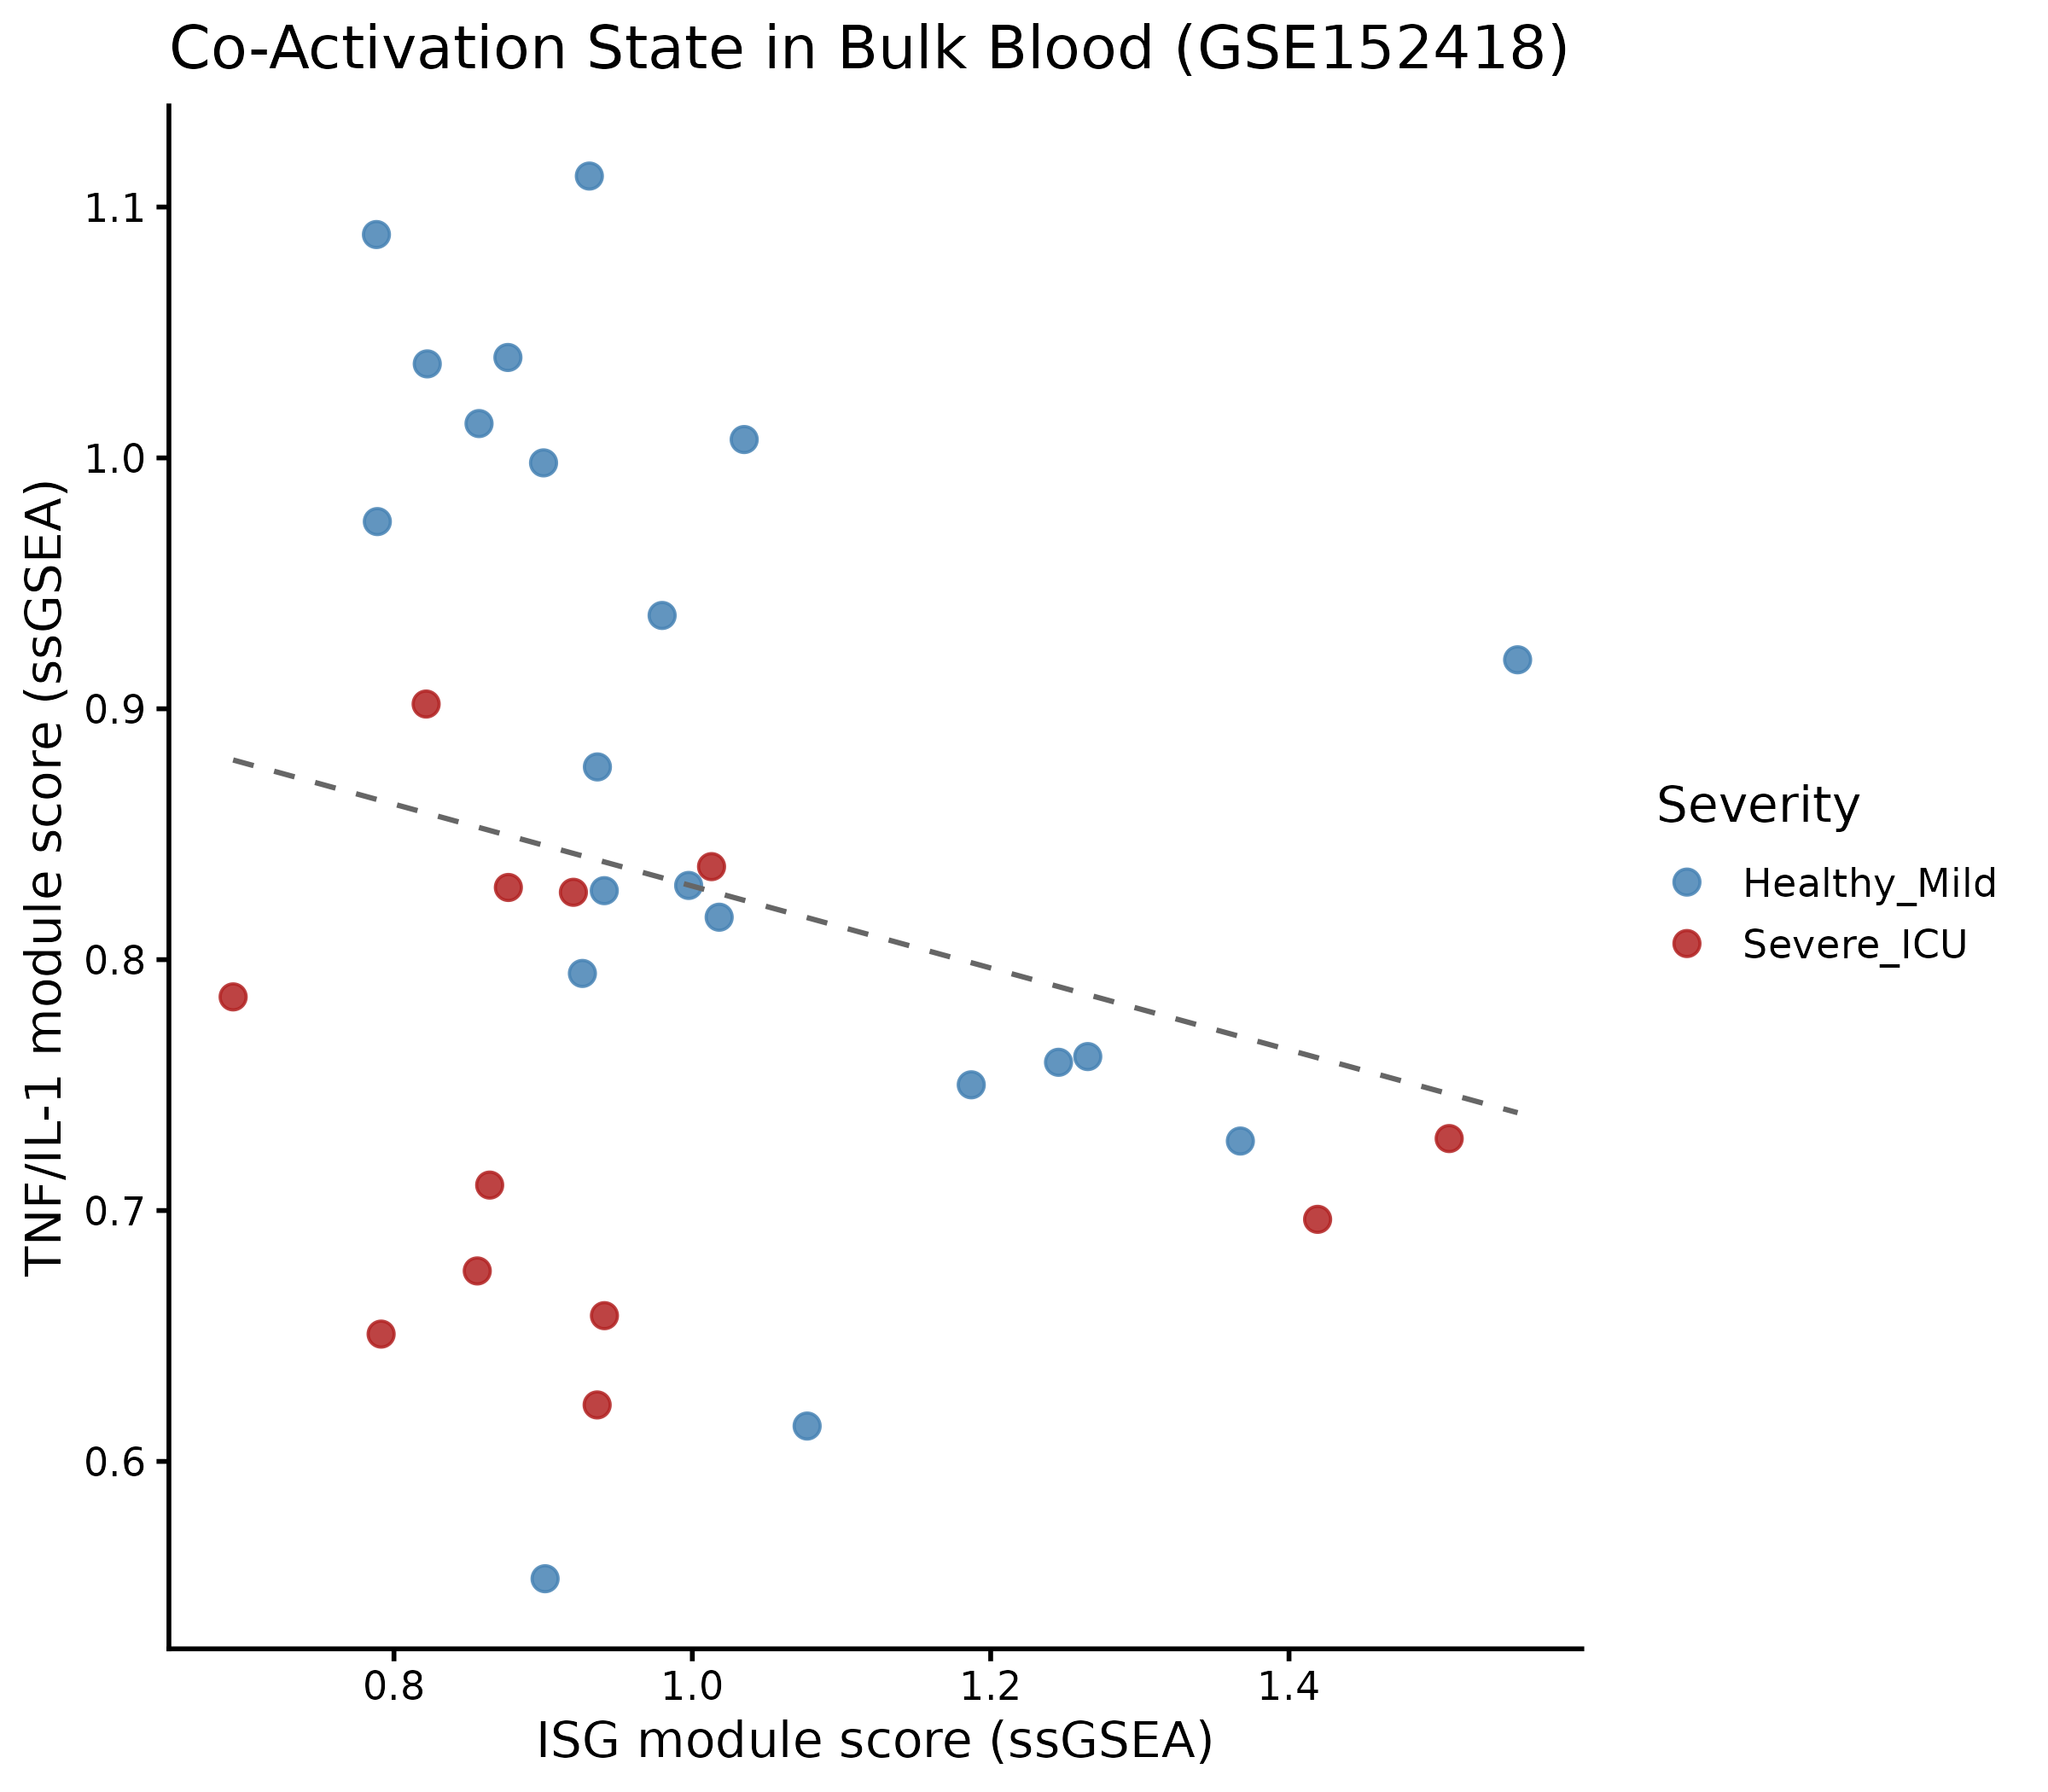
\includegraphics[width=0.82\textwidth]{plots/phase13/phase13_coactivation_scatter_GSE152418.png}
\end{center}

Each dot is one whole-blood sample.
Healthy/Mild samples (blue) occupy the \textbf{upper half} — higher TNF/IL-1$\beta$ scores.
Severe/ICU samples (red) fall to the \textbf{lower half}.
The co-activated upper-right quadrant (high ISG \textit{and} high TNF/IL-1$\beta$)
contains \textbf{no Severe samples}.

The trend line has a negative slope: ISG and TNF/IL-1$\beta$ enrichment are
\textit{inversely correlated} in bulk blood — the opposite of co-activation.
Samples with the most ISG signal are those with the most surviving lymphocytes, which
are by definition the milder cases.

Compare this directly to Phase 4: there, Severe monocytes pushed into the top-left
(high inflammation, low ISG) and top-right (co-activated). Here, Severe blood samples
fall to the bottom. The two scatters are mirror images because they measure the same
disease from different altitudes — cell level versus blood level.
ssGSEA, even with the exact Phase 4 gene lists and the most sensitive bulk scoring
method available, cannot detect the co-activation signal in whole blood.

% ═══════════════════════════════════════════════
\section{Conclusions}
% ═══════════════════════════════════════════════

The complete analysis — from raw 10X counts to bulk pathway enrichment — answers the
research question:

\begin{quote}
\textit{Yes, severe COVID-19 is associated with a classical monocyte state showing
simultaneous ISG and TNF/IL-1$\beta$ co-activation. This state is real, confirmed
in an independent cohort (GSE150861), and selectively suppressed by Tocilizumab
within four days. However, it is a \textbf{minority signal within a minority cell type},
completely masked in whole-blood bulk RNA-seq by the dominant compositional shift
(monocyte expansion + lymphocyte depletion). Detecting it required single-cell resolution.}
\end{quote}

\begin{enumerate}[nosep]
  \item \textbf{Severe COVID reshapes the blood immune landscape.}
        Monocytes expand from $\sim$35\% to $\sim$50\%; CD4$^+$ T cells deplete from
        $\sim$12\% to $\sim$5\%. This shift is already visible in the UMAP (Phase 4)
        and confirmed quantitatively in bulk PCA where PC1 separates severity with
        zero overlap (Phase 11, 97\% clustering accuracy).

  \item \textbf{Monocyte dysregulation is sub-cluster-specific.}
        Ten monocyte sub-clusters were identified: IL-1$\beta^+$ inflammasome-active
        (cluster~7), ISG-high (cluster~10), and chemokine-secreting (cluster~18).
        The ISG and inflammatory programs live in distinct monocyte sub-populations.

  \item \textbf{Mild and Severe COVID drive opposite monocyte programs.}
        ISG activity peaks in Mild COVID; TNF/IL-1$\beta$ dominates Severe.
        The worst outcomes are linked to unchecked inflammation, not sustained antiviral defense.

  \item \textbf{Co-activation is reproducible and treatment-responsive.}
        GSE150861 confirms $\sim$30\% co-activation on Day 1; Tocilizumab reduces this to
        near zero within four days by suppressing TNF/IL-1$\beta$ while leaving ISG
        intact — mechanistic evidence of independent regulation.

  \item \textbf{Severe COVID monocytes undergo immunoparalysis.}
        3,269 DE genes show IL1B and CXCL8 gained while HLA-DQ and KLF2 are lost.
        Monocytes become hyper-inflammatory yet lose antigen-presenting capacity.

  \item \textbf{Bulk RNA-seq captures composition, not co-activation.}
        The dominant bulk signal is myeloid/platelet expansion, coagulation activation,
        and lymphocyte depletion — confirmed by DESeq2, GSEA, and ssGSEA.
        The monocyte co-activation programs are net-lower in Severe bulk blood.
        Single-cell resolution was indispensable for the central finding of this project.
\end{enumerate}

\end{document}
